% !TeX program = xelatex
% !TeX TXS-program:compile = txs:///xelatex/[--shell-escape]
%%%%%%%%%%%%%%%%%%%%%%%%%%%%%%%%%%%%%%%%%%%%%%%%%%%%%%%%%%%%%%%%%%%%%%%%
% Plantilla TFG/TFM
% Escuela Politécnica Superior de la Universidad de Alicante
% Realizado por: Jose Manuel Requena Plens
% Contacto: info@jmrplens.com / Telegram:@jmrplens
%%%%%%%%%%%%%%%%%%%%%%%%%%%%%%%%%%%%%%%%%%%%%%%%%%%%%%%%%%%%%%%%%%%%%%%%

% Elige si deseas optimizar la ejecución del proyecto almacenando las figuras generadas con TikZ y PGF en una carpeta (archivos/figuras-procesadas).
% 1 - Si, 2 - No
\def\OptimizaTikZ{1}

% Archivo .TEX que incluye todas las configuraciones del documento y los paquetes. Añade todo aquello que necesites utilizar en el documento en este archivo.
% En él se encuentra la configuración de los márgenes, establecidos según las directrices de estilo de la EPS.
%%%%%%%%%%%%%%%%%%%%%%%%%%%%%%%%%%%%%%%%%%%%%%%%%%%%%%%%%%%%%%%%%%%%%%%%
% Plantilla TFG/TFM
% Escuela Politécnica Superior de la Universidad de Alicante
% Realizado por: Jose Manuel Requena Plens
% Contacto: info@jmrplens.com / Telegram:@jmrplens
%%%%%%%%%%%%%%%%%%%%%%%%%%%%%%%%%%%%%%%%%%%%%%%%%%%%%%%%%%%%%%%%%%%%%%%%

%%%%%%%%%%%%%%%%%%%%%%%%
% FORMATO DEL DOCUMENTO
%%%%%%%%%%%%%%%%%%%%%%%%
% scrbook es la clase de documento
% Si se desea que no haya página en blanco entre capítulos añadir "openany" en los parámetros de la clase. Sino siempre los capítulos empezarán en página impar.
\documentclass[a4paper,11pt,titlepage]{scrbook}
\KOMAoption{toc}{bib,chapterentryfill} % Opciones del índice
\usepackage{scrhack} % Previene algunos errores
% Paquete de formato para scrbook. Con marcas, linea-separador superior e inferior
\usepackage[automark,headsepline,footsepline]{scrlayer-scrpage}
\clearpairofpagestyles		% Borra los estilos por defecto
%%
% Formato y contenido de la información de cabecera y pie de página
%%
% Información de capítulo en cabecera e interno
\ihead{{\color{gray30}\scshape\small\headmark}}	
% Número de página en cabecera y externo
\ohead{\normalfont\pagemark} 
% Número de página en pie de página y externo. Sólo en páginas sin cabecera
\ofoot[\normalfont\pagemark]{}
%% 		
% Edición del contenido de las distintas partes de la cabecera
%%
\renewcommand{\chaptermark}[1]{\markboth{#1}{}} % Capítulo (Solo texto)
\renewcommand{\sectionmark}[1]{\markright{\thesection. #1}} % Sección (Número y texto)
\setkomafont{pagenumber}{} % Número de página (Sin nada añadido)

% Añade al índice y numera hasta la profundidad 4.
% 1:section,2:subsection,3:subsubsection,4:paragraph
\setcounter{tocdepth}{4}
\setcounter{secnumdepth}{4}
% Muestra una regla para comprobar el formato de las páginas
%\usepackage[type=upperleft,showframe,marklength=8mm]{fgruler}
% MÁRGENES DE LAS PÁGINAS
\usepackage[
  inner	=	3.0cm, % Margen interior
  outer	=	2.5cm, % Margen exterior
  top	=	2.5cm, % Margen superior
  bottom=	2.5cm, % Margen inferior
  includeheadfoot, % Incluye cabecera y pie de página en los márgenes
]{geometry}
% Valor de interlineado
\renewcommand{\baselinestretch}{1.0} % 1 línea de interlineado
% Para poder generar páginas horizontales
\usepackage{lscape}
% Ancho de la zona para comentarios en el margen. (modificado para todonotes)
\setlength{\marginparwidth}{2cm}

%%%%%%%%%%%%%%%%%%%%%%%%
% BIBLIOGRAFÍA
%%%%%%%%%%%%%%%%%%%%%%%%
\usepackage{apacite} % NORMA APA
\usepackage{natbib}
\usepackage{breakcites}

%%%%%%%%%%%%%%%%%%%%%%%%
% DOCUMENTO EN ESPAÑOL
%%%%%%%%%%%%%%%%%%%%%%%%
\usepackage[base]{babel}
\usepackage{polyglossia}
\setdefaultlanguage{spanish}

\addto\captionsspanish{%
	\renewcommand{\listtablename}{Índice de tablas} 
	\renewcommand{\tablename}{Tabla}
	\renewcommand{\lstlistingname}{Código}
	\renewcommand{\lstlistlistingname}{Índice de \lstlistingname s}
	\renewcommand{\glossaryname}{Glosario}
	\renewcommand{\acronymname}{Acrónimos}
	\renewcommand{\bibname}{Bibliografía}%
}

%%%%%%%%%%%%%%%%%%%%%%%% 
% COLORES
%%%%%%%%%%%%%%%%%%%%%%%% 
% Biblioteca de colores
\usepackage{color}
\usepackage[dvipsnames]{xcolor}
% Otros colores definidos por el usuario
\definecolor{gray97}{gray}{.97}
\definecolor{gray75}{gray}{.75}
\definecolor{gray45}{gray}{.45}
\definecolor{gray30}{gray}{.30}
\definecolor{negro}{RGB}{0,0,0}
\definecolor{blanco}{RGB}{255,255,255}
\definecolor{dkgreen}{rgb}{0,.6,0}
\definecolor{dkblue}{rgb}{0,0,.6}
\definecolor{dkyellow}{cmyk}{0,0,.8,.3}
\definecolor{gray}{rgb}{0.5,0.5,0.5}
\definecolor{mauve}{rgb}{0.58,0,0.82}
\definecolor{deepblue}{rgb}{0,0,0.5}
\definecolor{deepred}{rgb}{0.6,0,0}
\definecolor{deepgreen}{rgb}{0,0.5,0}
\definecolor{MyDarkGreen}{rgb}{0.0,0.4,0.0}
\definecolor{bluekeywords}{rgb}{0.13,0.13,1}
\definecolor{greencomments}{rgb}{0,0.5,0}
\definecolor{redstrings}{rgb}{0.9,0,0}

%%%%%%%%%%%%%%%%%%%%%%%%
% TABLAS
%%%%%%%%%%%%%%%%%%%%%%%%
% Paquetes para tablas
\usepackage{longtable,booktabs,array,multirow,multicol,tabularx,ragged2e,array}
% Nuevos tipos de columna para tabla, se pueden utilizar como por ejemplo C{3cm} en la definición de columnas de la función tabular
\newcolumntype{L}[1]{>{\raggedright\let\newline\\\arraybackslash\hspace{0pt}}m{#1}}
\newcolumntype{C}[1]{>{\centering\let\newline\\\arraybackslash\hspace{0pt}}m{#1}}
\newcolumntype{R}[1]{>{\raggedleft\let\newline\\\arraybackslash\hspace{0pt}}m{#1}}

%%%%%%%%%%%%%%%%%%%%%%%% 
% GRAFICAS y DIAGRAMAS 
%%%%%%%%%%%%%%%%%%%%%%%% 
% Paquete para todo tipo de gráficas, diagramas, modificación de imágenes, etc
\usepackage{tikz,tikzpagenodes}
\usetikzlibrary{tikzmark,calc,shapes.geometric,arrows,backgrounds,shadings,shapes.arrows,shapes.symbols,shadows,positioning,fit,automata,patterns,intersections}
\usepackage{pgfplots}
\pgfplotsset{colormap/jet}
\pgfplotsset{compat=newest} % Compatibilidad
\usepgfplotslibrary{patchplots,groupplots,fillbetween,polar}
\usepackage{pgfplotstable}
% Guardar las figuras realizadas con Tikz y Pgf en una carpeta externa
% para agilizar el procesado y tenerlas para utilizarlas en otros
% documentos
\if\OptimizaTikZ 1
\usepgfplotslibrary{external}
\tikzset{%
    external/system call ={xelatex -enable-write18 -halt-on-error -interaction=batchmode -jobname "\image" "\texsource"},
}
\fi

% Estilos para elementos graficos
% Cajas y cajas de texto
\tikzstyle{Caja1} = [green,very thick,rounded corners,fill=white, fill opacity=0.5]
\tikzstyle{Texto1} = [fill=white,thick,shape=circle,draw=black,inner sep=2pt,font=\sffamily,text=black]
\tikzstyle{Texto2} = [fill=white,thick,shape=rectangle,draw=black,inner sep=2pt,font=\sffamily,text=black]
\tikzstyle{Texto3} = [fill=white,thick,shape=circle,draw=black,inner sep=2pt,font=\sffamily,text=black]
% Cuadros de diagrama
\tikzstyle{rectvioleta} = [rectangle, rounded corners, text centered, draw=black, fill=blue!10]
\tikzstyle{rectnaranja} = [rectangle, minimum width=2cm, minimum height=1cm, text centered, draw=black, fill=orange!10]
\tikzstyle{romborosa} = [diamond, aspect=3, minimum width=3cm, minimum height=1cm, text centered, draw=black, fill=red!10]
\tikzstyle{rectverde} = [rectangle, minimum width=2cm, minimum height=1cm, text centered, draw=black, fill=green!10]
\tikzstyle{rectamarillo} = [rectangle, rounded corners, minimum width=2cm, minimum height=1cm, text centered, draw=black, fill=yellow!10]
% Flechas
\tikzstyle{arrow} = [thick,->,>=stealth]

%%%%%%%%%%%%%%%%%%%%%%%% 
% FIGURAS, TABLAS, ETC 
%%%%%%%%%%%%%%%%%%%%%%%% 
\usepackage{subcaption} % Para poder realizar subfiguras
\usepackage{caption} % Para aumentar las opciones de diseño
% Nombres de figuras, tablas, etc, en negrita la numeración, todo con letra small
\captionsetup{labelfont={bf,small},textfont=small}
% Paquete para modificar los espacios arriba y abajo de una figura o tabla
\usepackage{setspace}
% Define el espacio tanto arriba como abajo de las figuras, tablas
\setlength{\intextsep}{5mm}
% Para ajustar tamaños de texto de toda una tabla o grafica
% Uso: {\scalefont{0.8} \begin{...} \end{...} }
\usepackage{scalefnt}
% Redefine las tablas y figuras para eliminar el '.' entre la numeración y el texto
\renewcommand*{\figureformat}{\figurename~\thefigure}
\renewcommand*{\tableformat}{\tablename~\thetable}

%%%%%%%%%%%%%%%%%%%%%%%% 
% TEXTO
%%%%%%%%%%%%%%%%%%%%%%%%
% Paquete para poder modificar las fuente de texto
\usepackage{xltxtra}
% Cualquier tamaño de texto. Uso: {\fontsize{100pt}{120pt}\selectfont tutexto}
\usepackage{anyfontsize}
% Para modificar parametros del texto.
\usepackage{setspace}
% Paquete para posicionar bloques de texto
\usepackage{textpos}
% Paquete para realizar cajas de texto. 
% Uso: \begin{mdframed}[linecolor=red!100!black] tutexto \end{mdframed}
\usepackage{framed,mdframed}
% Para subrayar. Uso: \hlc[tucolor]{tutexto}
\newcommand{\hlc}[2][yellow]{ {\sethlcolor{#1} \hl{#2}} }

%%%%%%%%%%%%%%%%%%%%%%%% 
% OTROS
%%%%%%%%%%%%%%%%%%%%%%%%
% Para hacer una pagina horizontal. Uso: \begin{landscape} xxxx \end{lanscape}
\usepackage{lscape} 
% Para incluir paginas PDF. Uso:
% \includepdf[pages={1}]{tuarchivo.pdf}
\usepackage{pdfpages}
% Para introducir url's con formato. Uso: \url{http://www.google.es}
\usepackage{url}
% Amplia muchas funciones graficas de latex
\usepackage{graphicx}
% Paquete que añade el hipervinculo en referencias dentro del documento, indice, etc
% Se define sin bordes alrededor. Uso: \ref{tulabel}
\usepackage[pdfborder={000}]{hyperref}
\usepackage{float}
\usepackage{placeins}
\usepackage{afterpage}
\usepackage{verbatim}
% Paquete para condicionales avanzados
\usepackage{xstring,xifthen}
% Paquete para realizar calculos en el código
\usepackage{calc}
% Para rotar tablas o figuras o su contenido
\usepackage{rotating} 
% Para incluir comentarios en el texto. El parámetro 'disable' oculta todas las notas.
% USO: \todo{tutexto}
\usepackage[backgroundcolor=Apricot,textsize=tiny,spanish,shadow,loadshadowlibrary,textwidth=1.5cm]{todonotes}
%\reversemarginpar % Descomentar si se quiere todos los comentarios en el mismo lado
% Desactiva la exportación de los ToDo y Missingfigures como figuras
\if\OptimizaTikZ 1
\makeatletter
\renewcommand{\todo}[2][]{\tikzexternaldisable\@todo[#1]{#2}\tikzexternalenable}
\makeatother
\usepackage{letltxmacro}
\LetLtxMacro{\oldmissingfigure}{\missingfigure}
\makeatletter
\renewcommand{\missingfigure}[2][]{\tikzexternaldisable\oldmissingfigure[{#1}]{#2}\tikzexternalenable}
\makeatother
\fi

%%%%%%%%%%%%%%%%%%%%%%%% 
% GLOSARIOS
%%%%%%%%%%%%%%%%%%%%%%%%
\usepackage[acronym,nonumberlist,toc]{glossaries}
\usepackage{glossary-superragged}
\newglossarystyle{modsuper}{%
  \setglossarystyle{super}%
  \renewcommand{\glsgroupskip}{}
}
\renewcommand{\glsnamefont}[1]{\textbf{#1}}

%%%%%%%%%%%%%%%%%%%%%%%% 
% COMANDOS AÑADIDOS
%%%%%%%%%%%%%%%%%%%%%%%%
% Para mostrar la fecha actual (mes año) con \Hoy
\newcommand{\MES}{%
  \ifcase\month% 0
    \or Enero% 1
    \or Febrero% 2
    \or Marzo% 3
    \or Abril% 4
    \or Mayo% 5
    \or Junio% 6
    \or Julio% 7
    \or Agosto% 8
    \or Septiembre% 9
    \or Octubre% 10
    \or Noviembre% 11
    \or Diciembre% 12
  \fi}
\newcommand{\ANYO}{\number\year}
\newcommand{\Hoy}{\MES\ \ANYO}

%%%%%%%%%%%%%%%%%%%%%%%% 
% MATEMÁTICAS
%%%%%%%%%%%%%%%%%%%%%%%%
\usepackage{mathtools,amsthm,amsfonts,amssymb,bm,mathrsfs,nicefrac,upgreek,bigints} 
% Comando para añadir información de variables a las ecuaciones
% Uso: \begin{condiciones}[donde:] ....... \end{condiciones}
\newenvironment{condiciones}[1][2]
  {%
   #1\tabularx{\textwidth-\widthof{#1}}[t]{
     >{$}l<{$} @{}>{${}}c<{{}$}@{} >{\raggedright\arraybackslash}X
   }%
  }
  {\endtabularx\\[\belowdisplayskip]}

%%%%%
% PARÁMETROS DE FORMATO DE CODIGOS
%%%%%
% Puedes editar los formatos para ajustarlos a tu gusto
%%%%%%%%%%%%%%%%%%%%%%%%%%%%%%%%%%%%%%%%%%%%%%%%%%%%%%%%%%%%%%%%%%%%%%%%
% Plantilla TFG/TFM
% Escuela Politécnica Superior de la Universidad de Alicante
% Realizado por: Jose Manuel Requena Plens
% Contacto: info@jmrplens.com / Telegram:@jmrplens
%%%%%%%%%%%%%%%%%%%%%%%%%%%%%%%%%%%%%%%%%%%%%%%%%%%%%%%%%%%%%%%%%%%%%%%%


%%%%%%%%%%%%%%%%%%%%%%%% 
% CÓDIGO. CONFIGURACIÓN. En el siguiente bloque están los estilos.
%%%%%%%%%%%%%%%%%%%%%%%%
% Paquete para mostrar código de matlab. En caja y lineas numeradas
\usepackage[framed,numbered]{matlab-prettifier}
% Paquete mostrar código de programación de distintos lenguajes
\usepackage{listings}
\lstset{ inputencoding=utf8,
extendedchars=true,
frame=single, % Caja donde se ubica el código
backgroundcolor=\color{gray97}, % Color del fondo de la caja
rulesepcolor=\color{black},
boxpos=c,
abovecaptionskip=-4pt,
aboveskip=12pt,
belowskip=0pt,
lineskip=0pt,
framerule=0pt,
framextopmargin=4pt,
framexbottommargin=4pt,
framexleftmargin=11pt,
framexrightmargin=0pt,
linewidth=\linewidth,
xleftmargin=\parindent,
framesep=0pt,
rulesep=.4pt,
stringstyle=\ttfamily,
showstringspaces = false,
showspaces = false,
showtabs = false,
columns=fullflexible,
basicstyle=\small\ttfamily,
commentstyle=\color{gray45},
keywordstyle=\bfseries,
tabsize=4,
numbers=left,
numbersep=1pt,
numberstyle=\tiny\ttfamily\color{gray75},
numberfirstline = false,
breaklines=true,
postbreak=\mbox{\textcolor{red}{$\hookrightarrow$}\space}, % Flecha al saltar de linea
prebreak=\mbox{\textcolor{red}{$\hookleftarrow$}\space}, % Flecha al saltar de linea
literate=
  {á}{{\'a}}1 {é}{{\'e}}1 {í}{{\'i}}1 {ó}{{\'o}}1 {ú}{{\'u}}1
  {Á}{{\'A}}1 {É}{{\'E}}1 {Í}{{\'I}}1 {Ó}{{\'O}}1 {Ú}{{\'U}}1
  {à}{{\`a}}1 {è}{{\`e}}1 {ì}{{\`i}}1 {ò}{{\`o}}1 {ù}{{\`u}}1
  {À}{{\`A}}1 {È}{{\'E}}1 {Ì}{{\`I}}1 {Ò}{{\`O}}1 {Ù}{{\`U}}1
  {ä}{{\"a}}1 {ë}{{\"e}}1 {ï}{{\"i}}1 {ö}{{\"o}}1 {ü}{{\"u}}1
  {Ä}{{\"A}}1 {Ë}{{\"E}}1 {Ï}{{\"I}}1 {Ö}{{\"O}}1 {Ü}{{\"U}}1
  {â}{{\^a}}1 {ê}{{\^e}}1 {î}{{\^i}}1 {ô}{{\^o}}1 {û}{{\^u}}1
  {Â}{{\^A}}1 {Ê}{{\^E}}1 {Î}{{\^I}}1 {Ô}{{\^O}}1 {Û}{{\^U}}1
  {œ}{{\oe}}1 {Œ}{{\OE}}1 {æ}{{\ae}}1 {Æ}{{\AE}}1 {ß}{{\ss}}1
  {ű}{{\H{u}}}1 {Ű}{{\H{U}}}1 {ő}{{\H{o}}}1 {Ő}{{\H{O}}}1
  {ç}{{\c c}}1 {Ç}{{\c C}}1 {ø}{{\o}}1 {å}{{\r a}}1 {Å}{{\r A}}1
  {€}{{\euro}}1 {£}{{\pounds}}1 {«}{{\guillemotleft}}1
  {»}{{\guillemotright}}1 {ñ}{{\~n}}1 {Ñ}{{\~N}}1 {¿}{{?`}}1,
  }

% Intenta no dividir los códigos en diferentes paginas si es posible
\lstnewenvironment{listing}[1][]
   {\lstset{#1}\pagebreak[0]}{\pagebreak[0]}

% Formato de títulos de los códigos
\DeclareCaptionFont{white}{\color{white}}
\DeclareCaptionFormat{listing}{\colorbox{gray}{\parbox{\textwidth - 2\fboxsep}{#1#2#3}}}
\captionsetup[lstlisting]{format=listing,labelfont=white,textfont=white,font= scriptsize}


%%%%%%%%%%%%%%%%%%%%%%%% 
% CÓDIGO. ESTILOS. Ajústalos a tu gusto
%%%%%%%%%%%%%%%%%%%%%%%%
\lstdefinestyle{Consola}
	{
	basicstyle=\scriptsize\bf\ttfamily,
	}
   
\lstdefinestyle{C}
	{
	basicstyle=\scriptsize,
	language=C,
	}
\lstdefinestyle{C-color}
	{
  	breaklines=true,
  	language=C,
  	basicstyle=\scriptsize,
  	keywordstyle=\bfseries\color{green!40!black},
  	commentstyle=\itshape\color{purple!40!black},
  	identifierstyle=\color{blue},
  	stringstyle=\color{orange},
    }
\lstdefinestyle{CSharp}
	{
	basicstyle=\scriptsize
	language=[Sharp]C,
	escapeinside={(*@}{@*)},
	keywordstyle=\bfseries,
	}
\lstdefinestyle{CSharp-color}
	{
	basicstyle=\scriptsize
	language=[Sharp]C,
	escapeinside={(*@}{@*)},
	commentstyle=\color{greencomments},
	keywordstyle=\color{bluekeywords}\bfseries,
	stringstyle=\color{redstrings},
	}
\lstdefinestyle{C++}
	{
	basicstyle=\scriptsize,
	language=C++,
 	}
 	
\lstdefinestyle{C++-color}
	{
  	breaklines=true,
  	language=C++,
  	basicstyle=\scriptsize,
  	keywordstyle=\bfseries\color{green!40!black},
  	commentstyle=\itshape\color{purple!40!black},
  	identifierstyle=\color{blue},
  	stringstyle=\color{orange},
    }
    
\lstdefinestyle{PHP}
	{
	basicstyle=\scriptsize,
	language=PHP,
	}
	
\lstdefinestyle{PHP-color}
	{
	basicstyle=\scriptsize,
	language=PHP,
	keywordstyle    = \color{dkblue},
  	stringstyle     = \color{red},
  	identifierstyle = \color{dkgreen},
  	commentstyle    = \color{gray},
  	emph            =[1]{php},
  	emphstyle       =[1]\color{black},
  	emph            =[2]{if,and,or,else},
  	emphstyle       =[2]\color{dkyellow}
  }
  
\lstdefinestyle{Matlab}
	{
	basicstyle=\scriptsize,
	language=Matlab,
	numberstyle=\tiny\ttfamily\color{gray75},
	}
	
\lstdefinestyle{Matlab-color}
	{
	style = Matlab-editor,
	basicstyle=\scriptsize,
	numberstyle=\tiny\ttfamily\color{gray75},
	}
	
\lstdefinestyle{Latex}
	{
	language=[LaTeX]{Tex},
    basicstyle=\scriptsize,
    literate={\$}{{{\bfseries\$}}}1,
    alsoletter={\\,*,\&},
    emph =[1]{\\begin,\\end,\\caption,\\label,\\centering,\\FloatBarrier,
              \\lstinputlisting,\\scalefont,\\addplot,\\input,
              \\legend,\\item,\\subitem,\\includegraphics,\\textwidth,
              \\section,\\subsection,\\subsubsection,\\paragraph,
              \\cite,\\citet,\\citep,\\gls,\\bibliographystyle,\\url,
              \\citet*,\\citep*,\\todo,\\missingfigure,\\footnote},
  	emphstyle =[1]\bfseries,
  	emph = [2]{equation,subequations,eqnarray,figure,subfigure,
  			   condiciones,flalign,tikzpicture,axis,lstlisting,
  			   itemize,description
  			   },
  	emphstyle =[2]\bfseries,
    numbers=none,
	}
	
\lstdefinestyle{Latex-color}
	{
	language=[LaTeX]{Tex},
    basicstyle=\scriptsize,
    commentstyle=\color{dkgreen},
    identifierstyle=\color{black},
    literate={\$}{{{\bfseries\color{Dandelion}\$}}}1, % Colorea el simbolo dollar
    alsoletter={\\,*,\&},
    emph =[1]{\\begin,\\end,\\caption,\\label,\\centering,\\FloatBarrier,
              \\lstinputlisting,\\scalefont,\\addplot,\\input,
              \\legend,\\item,\\subitem,\\includegraphics,\\textwidth,
              \\section,\\subsection,\\subsubsection,\\paragraph,
              \\cite,\\citet,\\citep,\\gls,\\bibliographystyle,\\url,
              \\citet*,\\citep*,\\todo,\\missingfigure,\\footnote},
  	emphstyle =[1]\bfseries\color{RoyalBlue},
  	emph = [2]{equation,subequations,eqnarray,figure,subfigure,
  			   condiciones,flalign,tikzpicture,axis,lstlisting,
  			   itemize,description
  			   },
  	emphstyle =[2]\bfseries,
    numbers=none,
	}
\lstdefinestyle{Java}
{
	basicstyle=\scriptsize,
	language=Java,
}

\lstdefinestyle{Java-color}
{
	basicstyle=\scriptsize,
	language=Java,
  	keywordstyle=\color{blue},
  	commentstyle=\color{dkgreen},
  	stringstyle=\color{mauve},
}
\lstdefinestyle{Python}
{
	language=Python,
	basicstyle=\scriptsize,
	otherkeywords={self},  
	keywordstyle=\bfseries,     
	emphstyle=\bfseries,    
	emph={MyClass,__init__},         
}

\lstdefinestyle{Python-color}
{
	language=Python,
	basicstyle=\scriptsize,
	otherkeywords={self},          
	keywordstyle=\bfseries\color{deepblue},
	emph={MyClass,__init__},         
	emphstyle=\bfseries\color{deepred},    
	stringstyle=\color{deepgreen},
}
\lstdefinestyle{R}
{
	language=R,                     
  	basicstyle=\scriptsize,
  	keywordstyle=\bfseries, 
}
\lstdefinestyle{R-color}
{
	language=R,                     
  	basicstyle=\scriptsize,
  	keywordstyle=\bfseries\color{RoyalBlue}, 
  	commentstyle=\color{YellowGreen},
  	stringstyle=\color{ForestGreen}  
}


%%%%%
% DEFINICION DE CONCEPTOS
%%%%
% Uso ejemplo: \begin{ejemplo} tucontenido \end{ejemplo} 
\newtheorem{teorema}{Teorema}[chapter]
\newtheorem{ejemplo}{Ejemplo}[chapter]
\newtheorem{definicion}{Definición}[chapter]

%%%%%
% MIS MODIFICACIONES
%%%%%
% Añadir espaciado entre párrafos
% \setlength{\parskip}{2ex plus0.7ex minus0.4ex}
% \setlength{\parskip}{0.5ex plus0.2ex minus0.1ex}
% Cambio formato a la primera aparición de un acrónimo, primero siglas, luego descripción entre paréntesis
\renewcommand{\acrfullformat}[2]{#2\space(#1)}

% Añadir índices y caption para Ecuaciones
\usepackage{amsmath}
\DeclareCaptionType{customequation}[][Lista de ecuaciones]
\DeclareCaptionLabelFormat{customequationformat}{#1 #2}
\captionsetup[customequation]{name={Ecuación}, labelformat=customequationformat}

% \usepackage{xcolor}
% \DeclareCaptionFont{blue}{\color{blue}}
% \captionsetup{labelfont={blue,bf}}


% \DeclareCaptionFormat{listing}{\rule{\dimexpr\textwidth+17pt\relax}{0.4pt}\par\vskip1pt#1#2#3}
% \captionsetup[lstlisting]{format=listing,singlelinecheck=false, margin=0pt, font={sf},labelsep=space,labelfont=bf}
% \definecolor{listinggray}{gray}{0.9}
% \definecolor{lbcolor}{rgb}{0.9,0.9,0.9}
% \lstset{
%   backgroundcolor=\color{lbcolor},
%   tabsize=4,    
% % rulecolor=,
%   language=[GNU]C++,
%   basicstyle=\scriptsize,
%   upquote=true,
%   aboveskip={1.5\baselineskip},
%   columns=fixed,
%   showstringspaces=false,
%   extendedchars=false,
%   breaklines=true,
%   prebreak = \raisebox{0ex}[0ex][0ex]{\ensuremath{\hookleftarrow}},
%   frame=single,
%   numbers=left,
%   showtabs=false,
%   showspaces=false,
%   showstringspaces=false,
%   identifierstyle=\ttfamily,
%   keywordstyle=\color[rgb]{0,0,1},
%   commentstyle=\color[rgb]{0.026,0.112,0.095},
%   stringstyle=\color[rgb]{0.627,0.126,0.941},
%   numberstyle=\color[rgb]{0.205, 0.142, 0.73},
% % \lstdefinestyle{C++}{language=C++,style=numbers}’.
% }
\lstset{
  backgroundcolor=\color[rgb]{0.9,0.9,0.9},
  tabsize=4,
  language=C++,
% captionpos=b,
  tabsize=3,
  frame=lines,
  numbers=left,
  numberstyle=\tiny,
  numbersep=5pt,
  breaklines=true,
  showstringspaces=false,
% basicstyle=\footnotesize,
% identifierstyle=\color{magenta},
  keywordstyle=\color[rgb]{0,0,1},
  commentstyle=\color{ForestGreen},
  stringstyle=\color{RedOrange}
}


% Obligatorio colocar en el main en la versión para Overleaf, no eliminar
\if\OptimizaTikZ 1
\tikzexternalize[prefix=archivos/figuras-procesadas/] % Ruta
\fi 

%%%%%%%%%%%%%%%%%%%%%%%%%%%%%%%%%%%%%%%%%%%%%%%%%%%%%%%%%%%%%%%%%%%%%%
% INFORMACIÓN DEL TFG
% Comentar lo que NO se desee añadir y sustituir con la información correcta.
%%%%%%%%%%%%%%%%%%%%%%%%%%%%%%%%%%%%%%%%%%%%%%%%%%%%%%%%%%%%%%%%%%%%%%
% Título y subtítulo
\newcommand{\titulo}{Reconstrucción del cuerpo humano utilizando datos RGB-D y GPUs}
\newcommand{\subtitulo}{Implementación del proyecto en una computadora de bajo coste.}
% Datos del autor
\newcommand{\miNombre}{Edgar Martínez Serrano}
\newcommand{\miEmail}{ems107@alu.ua.es}
% Datos del tutor/es
\newcommand{\miTutor}{Marcelo Saval Calvo}
\newcommand{\departamentoTutor}{Tecnología Informática y Computación}
\newcommand{\miTutorB}{Jorge Azorín López}
\newcommand{\departamentoTutorB}{Tecnología Informática y Computación}
% Datos de la facultada y universidad
\newcommand{\miFacultad}{Escuela Politécnica Superior}
\newcommand{\miFacultadCorto}{EPS UA}
\newcommand{\miUniversidad}{\protect{Universidad de Alicante}}
\newcommand{\miUbicacion}{Alicante}

%%%%%%%%%%%%%%%%%%%%%%%%%%%%%%%%%%%%%%%%%%%%%%%%%%%%%%%%%%%%%%%%%%%%%%
% INDICA TU TITULACIÓN
% ID	GRADO -------------------------------------------------
% 1		Ingeniería en Imagen y Sonido en Telecomunicación
% 2		Ingeniería Civil
% 3		Ingeniería Química
% 4		Ingeniería Informática
% 5		Ingeniería Multimedia
% 6		Arquitectura Técnica
% 7		Arquitectura
% 8		Robótica
% %		%%%%%%%%%%%%
% ID	MÁSTER ------------------------------------------------
% A		Telecomunicación
% B		Caminos, Canales y Puertos
% C		Gestión en la Edificación
% D		Desarrollo Web
% E		Materiales, Agua, Terreno
% F		Informática
% G 	Automática y Robótica
% H		Prevención de riesgos laborales
% I		Gestión Sostenible Agua
% J		Desarrollo Aplicaciones Móviles
% K		Ingeniería Química
% L		Ciberseguridad
%%%%%%%%%%%%%%%%%%%%%%%%%%%%%%%%%%%%%%%%%%%%%%%%%%%%%%%%%%%%%%%%%%%%%%%%%
%!!!!!!!!!!!!!!!!!!!!!!!!!!!!!!!!!!!!!!!!!!!!!!!!!!!!!!!!!!!!!!!!!!!!!%%%
																		%
\def\IDtitulo{4} % INTRODUCE LA ID DE TU TITULACIÓN						%
																		%
%!!!!!!!!!!!!!!!!!!!!!!!!!!!!!!!!!!!!!!!!!!!!!!!!!!!!!!!!!!!!!!!!!!!!!%%%
%%%%%%%%%%%%%%%%%%%%%%%%%%%%%%%%%%%%%%%%%%%%%%%%%%%%%%%%%%%%%%%%%%%%%%%%%

% Configuración automática según el identificador elegido
%%%%%%%%%%%%%%%%%%%%%%%%%%%%%%%%%%%%%%%%%%%%%%%%%%%%%%%%%%%%%%%%%%%%%%%%
% Plantilla TFG/TFM
% Escuela Politécnica Superior de la Universidad de Alicante
% Realizado por: Jose Manuel Requena Plens
% Contacto: info@jmrplens.com / Telegram:@jmrplens
%%%%%%%%%%%%%%%%%%%%%%%%%%%%%%%%%%%%%%%%%%%%%%%%%%%%%%%%%%%%%%%%%%%%%%%%

%%%%%%%%%%%%%%%%%%%%%%%% 
% COLORES DE GRADOS.
% Si el color de la titulación ha cambiado, modifícalo en las lineas siguientes.
%%%%%%%%%%%%%%%%%%%%%%%%
% Grados
\definecolor{teleco}{RGB}{32,2,116}			% Teleco
\definecolor{civil}{RGB}{201,56,140}			% Civil
\definecolor{quimica}{RGB}{41,199,255}		% Química
\definecolor{informatica}{RGB}{0,128,255}	% Informatica
\definecolor{multimedia}{RGB}{239,206,53}	% Multimedia
\definecolor{arquitecnica}{RGB}{0,179,148}	% Arquitectura técnica
\definecolor{arquitectura}{RGB}{181,0,0}		% Arquitectura
\definecolor{robotica}{RGB}{255,255,128}		% Robótica
% Másteres
\definecolor{masterteleco}{RGB}{32,2,116}	% Teleco
\definecolor{caminos}{RGB}{201,56,140}		% Caminos, Canales y Puertos
\definecolor{gestedif}{RGB}{50,120,50}		% Gestión Edificación
\definecolor{desweb}{RGB}{250,43,22}			% Desarrollo Web
\definecolor{mataguaterre}{RGB}{210,250,50}	% Materiales, Agua, Terreno
\definecolor{masterinfor}{RGB}{0,128,255}	% Informática
\definecolor{autorobo}{RGB}{83,145,201}		% Automática y Robótica
\definecolor{prevencion}{RGB}{0,100,0}		% Prevención Riesgos
\definecolor{gestionagua}{RGB}{7,138,197}	% Gestión Agua
\definecolor{moviles}{RGB}{121,11,21}		% Aplicaciones Móviles
\definecolor{masterquimica}{RGB}{41,199,255}	% Quimica
\definecolor{ciberseguridad}{RGB}{9,111,192}	% Ciberseguridad

% Logotipos comunes de todas las titulaciones
\newcommand{\logoFacultad}{include/logos-universidad/LogoEPSNegro}
\newcommand{\logoUniversidad}{include/logos-universidad/LogoUANegro}
\newcommand{\logoUniversidadPortada}{include/logos-universidad/LogoUABlanco}

% Colores generales
\definecolor{negro}{RGB}{0,0,0}
\definecolor{blanco}{RGB}{255,255,255}
%%%%%%%%%%%%%%%%%%%%%%%% 
% CONDICIONALES. SEGUN LA ID ELEGIDA EN EL .TEX PRINCIPAL
% Según el ID seleccionado en TFG_EPS_UA.tex se configurará el nombre de la titulación, logotipos y color.
% Si tu titulación no esta correctamente definida cambia las imágenes que se definen para tu titulación en las lineas de abajo
% Si deseas añadir mas titulaciones ve al final de este archivo
%%%%%%%%%%%%%%%%%%%%%%%%
% Grados
	\if\IDtitulo 1 % Teleco
		% Logos
		\newcommand{\logoFacultadPortada}{include/logos-universidad/LogoEPSBlanco}
		\newcommand{\logoGradoPortada}{include/logos-titulaciones/LogoTelecoBlanco}
		\newcommand{\logoGrado}{include/logos-titulaciones/LogoTelecoNegro}
		% Texto
		\newcommand{\miGrado}{Grado en Ingeniería en Sonido e Imagen en Telecomunicación}
		\newcommand{\tipotrabajo}{Trabajo Fin de Grado}
		% Color
		\newcommand{\colorgrado}{teleco}
		\newcommand{\colortexto}{blanco}
	\else \if\IDtitulo 2 % Civil
		\newcommand{\logoFacultadPortada}{include/logos-universidad/LogoEPSBlanco}
		\newcommand{\logoGradoPortada}{include/logos-titulaciones/LogoCivilBlanco}
		\newcommand{\logoGrado}{include/logos-titulaciones/LogoCivilNegro}
		% Texto
		\newcommand{\miGrado}{Grado en Ingeniería Civil}
		\newcommand{\tipotrabajo}{Trabajo Fin de Grado}
		% Color
		\newcommand{\colorgrado}{civil}
		\newcommand{\colortexto}{blanco}
	\else \if\IDtitulo 3 % Quimica
		% Logos
		\newcommand{\logoFacultadPortada}{include/logos-universidad/LogoEPSNegro}
		\newcommand{\logoGradoPortada}{include/logos-titulaciones/LogoQuimicaNegro}
		\newcommand{\logoGrado}{include/logos-titulaciones/LogoQuimicaNegro}
		% Texto
		\newcommand{\miGrado}{Grado en Ingeniería Química}
		\newcommand{\tipotrabajo}{Trabajo Fin de Grado}
		% Color
		\newcommand{\colorgrado}{quimica}
		\newcommand{\colortexto}{negro}
	\else \if\IDtitulo 4 % Informatica
		% Logos
		\newcommand{\logoFacultadPortada}{include/logos-universidad/LogoEPSBlanco}
		\newcommand{\logoGradoPortada}{include/logos-titulaciones/LogoInformaticaBlanco}
		\newcommand{\logoGrado}{include/logos-titulaciones/LogoInformaticaNegro}
		% Texto
		\newcommand{\miGrado}{Grado en Ingeniería Informática}
		\newcommand{\tipotrabajo}{Trabajo Fin de Grado}
		% Color
		\newcommand{\colorgrado}{informatica}
		\newcommand{\colortexto}{blanco}
	\else \if\IDtitulo 5 % Multimedia
		% Logos
		\newcommand{\logoFacultadPortada}{include/logos-universidad/LogoEPSNegro}
		\newcommand{\logoGradoPortada}{include/logos-titulaciones/LogoMultimediaNegro}
		\newcommand{\logoGrado}{include/logos-titulaciones/LogoMultimediaNegro}
		% Texto
		\newcommand{\miGrado}{Grado en Ingeniería Multimedia}
		\newcommand{\tipotrabajo}{Trabajo Fin de Grado}
		% Color
		\newcommand{\colorgrado}{multimedia}
		\newcommand{\colortexto}{negro}
	\else \if\IDtitulo 6 % Arquitectura Tecnica
		% Logos
		\newcommand{\logoFacultadPortada}{include/logos-universidad/LogoEPSBlanco}
		\newcommand{\logoGradoPortada}{include/logos-titulaciones/LogoArqTecnicaBlanco}
		\newcommand{\logoGrado}{include/logos-titulaciones/LogoArqTecnicaNegro}
		% Texto
		\newcommand{\miGrado}{Grado en Arquitectura Técnica}
		\newcommand{\tipotrabajo}{Trabajo Fin de Grado}
		% Color
		\newcommand{\colorgrado}{arquitecnica}
		\newcommand{\colortexto}{blanco}
	\else \if\IDtitulo 7 % Arquitectura
		% Logos
		\newcommand{\logoFacultadPortada}{include/logos-universidad/LogoEPSBlanco}
		\newcommand{\logoGradoPortada}{include/logos-titulaciones/LogoArquitecturaBlanco}
		\newcommand{\logoGrado}{include/logos-titulaciones/LogoArquitecturaNegro}
		% Texto
		\newcommand{\miGrado}{Grado en Arquitectura}
		\newcommand{\tipotrabajo}{Trabajo Fin de Grado}
		% Color
		\newcommand{\colorgrado}{arquitectura}
		\newcommand{\colortexto}{blanco}
	\else \if\IDtitulo 8 % Robotica
		% Logos
		\newcommand{\logoFacultadPortada}{include/logos-universidad/LogoEPSNegro}
		\newcommand{\logoGradoPortada}{include/logos-titulaciones/LogoRoboticaColor}
		\newcommand{\logoGrado}{include/logos-titulaciones/LogoRoboticaNegro}
		% Texto
		\newcommand{\miGrado}{Grado en Ingeniería Robótica}
		\newcommand{\tipotrabajo}{Trabajo Fin de Grado}
		% Color
		\newcommand{\colorgrado}{robotica}
		\newcommand{\colortexto}{negro}
% Másteres
	\else \if\IDtitulo A % Teleco
		% Logos
		\newcommand{\logoFacultadPortada}{include/logos-universidad/LogoEPSBlanco}
		\newcommand{\logoGradoPortada}{include/logos-titulaciones/LogoTelecoBlanco}
		\newcommand{\logoGrado}{include/logos-titulaciones/LogoTelecoNegro}
		% Texto
		\newcommand{\miGrado}{Máster Universitario en Ingeniería en Telecomunicación}
		\newcommand{\tipotrabajo}{Trabajo Fin de Máster}
		% Color
		\newcommand{\colorgrado}{masterteleco}
		\newcommand{\colortexto}{blanco}
	\else \if\IDtitulo B % Caminos, Canales y puertos
		% Logos
		\newcommand{\logoFacultadPortada}{include/logos-universidad/LogoEPSBlanco}
		\newcommand{\logoGradoPortada}{include/logos-titulaciones/LogoCivilBlanco}
		\newcommand{\logoGrado}{include/logos-titulaciones/LogoCivilNegro}
		% Texto
		\newcommand{\miGrado}{Máster Universitario en Ingeniería de Caminos, Canales y Puertos}
		\newcommand{\tipotrabajo}{Trabajo Fin de Máster}
		% Color
		\newcommand{\colorgrado}{caminos}
		\newcommand{\colortexto}{blanco}
	\else \if\IDtitulo C % Gestión Edificación
		% Logos
		\newcommand{\logoFacultadPortada}{include/logos-universidad/LogoEPSBlanco}
		\newcommand{\logoGradoPortada}{include/logos-titulaciones/LogoMasterEdificacionBlanco}
		\newcommand{\logoGrado}{include/logos-titulaciones/LogoMasterEdificacionNegro}
		\newcommand{\tipotrabajo}{Trabajo Fin de Máster}
		% Texto
		\newcommand{\miGrado}{Máster Universitario en Gestión de la Edificación}
		% Color
		\newcommand{\colorgrado}{gestedif}
		\newcommand{\colortexto}{blanco}
	\else \if\IDtitulo D % Desarrollo web
		% Logos
		\newcommand{\logoFacultadPortada}{include/logos-universidad/LogoEPSBlanco}
		\newcommand{\logoGradoPortada}{include/logos-titulaciones/LogoMasterDesarrolloBlanco}
		\newcommand{\logoGrado}{include/logos-titulaciones/LogoMasterDesarrolloNegro}
		% Texto
		\newcommand{\miGrado}{Máster Universitario en Desarrollo de Aplicaciones y Servicios Web}
		\newcommand{\tipotrabajo}{Trabajo Fin de Máster}
		% Color
		\newcommand{\colorgrado}{desweb}
		\newcommand{\colortexto}{blanco}
	\else \if\IDtitulo E % Materiales, Agua, Terreno
		% Logos
		\newcommand{\logoFacultadPortada}{include/logos-universidad/LogoEPSNegro}
		\newcommand{\logoGradoPortada}{include/logos-titulaciones/LogoMasterMaterialesNegro}
		\newcommand{\logoGrado}{include/logos-titulaciones/LogoMasterMaterialesNegro}
		% Texto
		\newcommand{\miGrado}{Máster Universitario en Ingeniería de los Materiales, del Agua y del Terreno}
		\newcommand{\tipotrabajo}{Trabajo Fin de Máster}
		% Color
		\newcommand{\colorgrado}{mataguaterre}
		\newcommand{\colortexto}{negro}
	\else \if\IDtitulo F % Informatica
		% Logos
		\newcommand{\logoFacultadPortada}{include/logos-universidad/LogoEPSBlanco}
		\newcommand{\logoGradoPortada}{include/logos-titulaciones/LogoInformaticaBlanco}
		\newcommand{\logoGrado}{include/logos-titulaciones/LogoInformaticaNegro}
		% Texto
		\newcommand{\miGrado}{Máster Universitario en Ingeniería Informática}
		\newcommand{\tipotrabajo}{Trabajo Fin de Máster}
		% Color
		\newcommand{\colorgrado}{masterinfor}
		\newcommand{\colortexto}{blanco}
	\else \if\IDtitulo G % Automática y Robótica
		% Logos
		\newcommand{\logoFacultadPortada}{include/logos-universidad/LogoEPSBlanco}
		\newcommand{\logoGradoPortada}{include/logos-titulaciones/LogoMasterRoboticaBlanco}
		\newcommand{\logoGrado}{include/logos-titulaciones/LogoMasterRoboticaNegro}
		% Texto
		\newcommand{\miGrado}{Máster Universitario en Automática y Robótica}
		\newcommand{\tipotrabajo}{Trabajo Fin de Máster}
		% Color
		\newcommand{\colorgrado}{autorobo}
		\newcommand{\colortexto}{blanco}
	\else \if\IDtitulo H % Prevención de riesgos laborales
		% Logos
		\newcommand{\logoFacultadPortada}{include/logos-universidad/LogoEPSBlanco}
		\newcommand{\logoGradoPortada}{include/logos-titulaciones/LogoMasterPrevencionBlanco}
		\newcommand{\logoGrado}{include/logos-titulaciones/LogoMasterPrevencionNegro}
		% Texto
		\newcommand{\miGrado}{Máster Universitario en Prevención de Riesgos Laborales}
		\newcommand{\tipotrabajo}{Trabajo Fin de Máster}
		% Color
		\newcommand{\colorgrado}{prevencion}
		\newcommand{\colortexto}{blanco}
	\else \if\IDtitulo I % Gestion Agua
		% Logos
		\newcommand{\logoFacultadPortada}{include/logos-universidad/LogoEPSNegro}
		\newcommand{\logoGradoPortada}{include/logos-titulaciones/LogoMasterAguaNegro}
		\newcommand{\logoGrado}{include/logos-titulaciones/LogoMasterAguaNegro}
		% Texto
		\newcommand{\miGrado}{Máster Universitario en Gestión Sostenible y Tecnologías del Agua}
		\newcommand{\tipotrabajo}{Trabajo Fin de Máster}
		% Color
		\newcommand{\colorgrado}{gestionagua}
		\newcommand{\colortexto}{negro}
	\else \if\IDtitulo J % Aplicaciones Móviles
		% Logos
		\newcommand{\logoFacultadPortada}{include/logos-universidad/LogoEPSBlanco}
		\newcommand{\logoGradoPortada}{include/logos-titulaciones/LogoMasterMovilesBlanco}
		\newcommand{\logoGrado}{include/logos-titulaciones/LogoMasterMovilesNegro}
		% Texto
		\newcommand{\miGrado}{Máster Universitario en Desarrollo de Software para Dispositivos Móviles}
		\newcommand{\tipotrabajo}{Trabajo Fin de Máster}
		% Color
		\newcommand{\colorgrado}{moviles}
		\newcommand{\colortexto}{blanco}
	\else \if\IDtitulo K % Quimica
		% Logos
		\newcommand{\logoFacultadPortada}{include/logos-universidad/LogoEPSNegro}
		\newcommand{\logoGradoPortada}{include/logos-titulaciones/LogoQuimicaNegro}
		\newcommand{\logoGrado}{include/logos-titulaciones/LogoQuimicaNegro}
		% Texto
		\newcommand{\miGrado}{Máster Universitario en Ingeniería Química}
		\newcommand{\tipotrabajo}{Trabajo Fin de Máster}
		% Color
		\newcommand{\colorgrado}{masterquimica}
		\newcommand{\colortexto}{negro}
	\else \if\IDtitulo L % Ciberseguridad
		% Logos
		\newcommand{\logoFacultadPortada}{include/logos-universidad/LogoEPSBlanco}
		\newcommand{\logoGradoPortada}{include/logos-titulaciones/LogoMasterCiberseguridadColor}
		\newcommand{\logoGrado}{include/logos-titulaciones/LogoMasterCiberseguridadNegro}
		% Texto
		\newcommand{\miGrado}{Máster Universitario en Ciberseguridad}
		\newcommand{\tipotrabajo}{Trabajo Fin de Máster}
		% Color
		\newcommand{\colorgrado}{ciberseguridad}
		\newcommand{\colortexto}{blanco}


	\fi \fi \fi \fi \fi \fi \fi \fi \fi \fi \fi \fi \fi \fi \fi \fi \fi \fi \fi \fi
	
%%%%%%%%%%%%%%%%%%%%%%%%%%%%%%%%%%%%%%%%%%%%%%%%%%%%%%%%%%%%%%%%%%%%%%%%	
% ¿COMO AÑADIR MÁS TITULACIONES?
% Para añadir más titulaciones, se debe continuar el el formato de ID -> Titulacion.
% Justo encima de la linea donde hay muchos '\fi' se debe escribir el condicional y el contenido de este tal que:
%
%	\else \if\IDtitulo X % Titulacion con ID=X		
% 		% Logos
%		\newcommand{\logoFacultadPortada}{include/logos-universidad/LogoEPSBlanco}
%		\newcommand{\logoGradoPortada}{include/logos-titulaciones/logotitulacion}
%		\newcommand{\logoGrado}{include/logos-titulaciones/logotitulacion}
%		% Texto
%		\newcommand{\miGrado}{Grado en XXXXXXXX}
%		\newcommand{\tipotrabajo}{Trabajo Fin de XXXX}
%		% Color
%		\newcommand{\colorgrado}{XXXX}
%		\newcommand{\colortexto}{XXX}
%	
% Por último añadir a la linea que tiene muchos '\fi', otro '\fi'. Listo, ya podrás usar la nueva ID con la configuración añadida.
%%%%%%%%%%%%%%%%%%%%%%%%%%%%%%%%%%%%%%%%%%%%%%%%%%%%%%%%%%%%%%%%%%%%%%%%	




 

% Información añadida a las propiedades del archivo PDF.
\hypersetup{
pdfauthor = {\miNombre~(\miEmail)},
pdftitle = {\titulo},
}

%%
% Archivo de acrónimos
%%
\makeglossaries % Genera la base de datos de acrónimos
% Lista de acrónimos (se ordenan por orden alfabético automáticamente)

% La forma de definir un acrónimo es la siguiente:
% \newacronym{id}{siglas}{descripción}
% Donde:
% 	'id' es como vas a llamarlo desde el documento.
%	'siglas' son las siglas del acrónimo.
%	'descripción' es el texto que representan las siglas.
%
% Para usarlo en el documento tienes 4 formas:
% \gls{id} - Añade el acrónimo en su forma larga y con las siglas si es la primera vez que se utiliza, el resto de veces solo añade las siglas. (No utilices este en títulos de capítulos o secciones).
% \glsentryshort{id} - Añade solo las siglas de la id
% \glsentrylong{id} - Añade solo la descripción de la id
% \glsentryfull{id} - Añade tanto  la descripción como las siglas

\newacronym{tfg}{TFG}{Trabajo Final de Grado}
\newacronym{2d}{2D}{Dos Dimensiones}
\newacronym{3d}{3D}{Tres Dimensiones}
\newacronym{tic}{TIC}{Técnología Informática y Computación}
\newacronym{taes}{TAES}{Técnicas Avanzadas de Especificación Software}
\newacronym{imcr}{IMCR}{Ingeniería de Mantenimiento de Computadores y Redes}
\newacronym{atc}{ATC}{Arquitectura y Tecnología de los Computadores}
\newacronym{is}{IS}{Ingeniería del Software}
\newacronym{rgb}{RGB}{Red Green Blue}
\newacronym{rgbd}{RGB-D}{Red Green Blue – Depth}
\newacronym{lidar}{LIDAR}{Light Detection And Ranging}
\newacronym{tof}{ToF}{Time of Flight}
\newacronym{cpu}{CPU}{Central Processing Unit}
\newacronym{gpu}{GPU}{Graphics Processing Unit}
\newacronym{ram}{RAM}{Random Access Memory}
\newacronym{cuda}{CUDA}{Compute Unified Device Architecture}
\newacronym{ididp}{IDIDP}{Ingeniería en Diseño Industrial y Desarrollo de Producto}
\newacronym{mclse}{MC-LSE}{Multi-Constraint Least Squares Estimation Algorithm}
\newacronym{dtic}{DTIC}{Departamento de Tecnología Informática y Computación}
\newacronym{ir}{IR}{Radiación Infrarroja}
\newacronym{pvp}{PVP}{Precio de Venta al Público}
\newacronym{upv}{UPV}{Universidad Politécnica de Valencia}
\newacronym{icp}{ICP}{Iterative Closest Point}
\newacronym{cpd}{CPD}{Coherent Point Drift}
\newacronym{fgt}{FGT}{Fast Gauss Transforms}
\newacronym{pcl}{PCL}{Point Cloud Library}
\newacronym{ransac}{RANSAC}{Random Sample Consensus}
\newacronym{pcd}{PCD}{Point Cloud Data}
\newacronym{ply}{PLY}{Polygon File Format}
\newacronym{gpgpu}{GPGPU}{General-Purpose Computing on Graphics Processing Units}
\newacronym{opencl}{OpenCL}{Open Computing Language}
\newacronym{sp}{SP}{Streaming Processors}
\newacronym{sm}{SM}{Streaming Multiprocessors}
\newacronym{simt}{SIMT}{Single Instruction Multiple Threads}
\newacronym{mmg}{MMG}{Modelo Mixto Gaussiana}
\newacronym{vcsel}{VCSEL}{Vertical Cavity Surface Emitting Laser}
 % Archivo que contiene los acrónimos

%%%%%%%%%%%%%%%%%%%%%%%% 
% INICIO DEL DOCUMENTO
% A partir de aquí debes empezar a realizar tu TFG/TFM
%%%%%%%%%%%%%%%%%%%%%%%%
\begin{document}

% Números romanos hasta el mainmatter.
\frontmatter

% PORTADA
%%%%%%%%%%%%%%%%%%%%%%%%%%%%%%%%%%%%%%%%%%%%%%%%%%%%%%%%%%%%%%%%%%%%%%%%
% Plantilla TFG/TFM
% Escuela Politécnica Superior de la Universidad de Alicante
% Realizado por: Jose Manuel Requena Plens
% Contacto: info@jmrplens.com / Telegram:@jmrplens
%%%%%%%%%%%%%%%%%%%%%%%%%%%%%%%%%%%%%%%%%%%%%%%%%%%%%%%%%%%%%%%%%%%%%%%%

%%%%%%%%%%%%%%%%%%%%%%%%
% PORTADA - no modificar
%%%%%%%%%%%%%%%%%%%%%%%%
% Establece las fuentes de texto de la portada
% Helvetica LS Std Cond. Uso: {\FuenteTitulo tutexto}
\newfontfamily\FuenteTitulo{HelveticaLTStd-Cond}[Path=./include/fuentes/]  
% Helvetica. Uso: {\FuentePortada tutexto}
\newfontfamily\FuentePortada{Helvetica}[Path=./include/fuentes/]  

% Ignora los márgenes establecidos para el documento. Después de la portada en blanco y negro (portada_bn.tex) devuelve los márgenes establecidos en configuracioninicial.tex
\newgeometry{ignoreall,top=2cm,outer=2cm,inner=2cm}

% Tamaño por defecto de la fuente de texto para:
\def\FuenteTamano{55pt}	% Tamaño para el título del trabajo
\def\interlinportada{5.0} % Interlineado por defecto para el título
\def\TamTrabajo{20pt} 	% Tamaño para el tipo de trabajo (grado o máster)
\def\TamTrabajoIn{20pt} 	% Tamaño para el salto de línea después de tipo de trabajo
\def\TamOtros{12pt} 	% Tamaño para datos personales y fecha
\def\TamOtrosIn{1pt} 	% Tamaño para los saltos de línea en la info personal

% Según la longitud del título se determina un tamaño e interlineado para él
\StrLen{\titulo}[\longitudtitulo] % Cuenta los caracteres título
% Comprueba la longitud del título y según sea este determina unos valores nuevos
\ifthenelse{\longitudtitulo > 180}{
\def\FuenteTamano{35pt}		% Si es mayor a 180 caracteres tamaño de fuente 35pt
\def\interlinportada{3.5}} 	% Establece nuevo interlineado
{\ifthenelse{\longitudtitulo > 140}{
\def\FuenteTamano{40pt}		% Si es mayor a 140 caracteres tamaño de fuente 40pt
\def\interlinportada{4.0}} 	% Establece nuevo interlineado
{\ifthenelse{\longitudtitulo > 120}{
\def\FuenteTamano{50pt}		% Si es mayor a 120 caracteres tamaño de fuente 50pt
\def\interlinportada{4.5}} 	% Establece nuevo interlineado
{} % Si no, no modifica el tamaño
} }

\if\OptimizaTikZ 1
\tikzexternaldisable % Desactiva la exportación com figura
\fi 

% Inicio de portada
\begin{titlepage}
% Offset horizontal para toda la portada
\newlength{\centeroffset}
\setlength{\centeroffset}{-0.5\oddsidemargin}
\addtolength{\centeroffset}{0.5\evensidemargin}
\thispagestyle{empty}

% Fondo del color del grado
\pagecolor{\colorgrado}
% Logo de la facultad en la esquina superior derecha
\begin{tikzpicture}[remember picture,overlay]
   \node[anchor=north west,inner sep=0pt] at ($(current page.north west)+(13.65cm,-1.4cm)$)
              {\includegraphics[width=5.3cm]{\logoFacultadPortada}};
\end{tikzpicture}

% Titulo y subtitulo
\hspace{0pt}
\vfill
\hspace{-0.8cm}\begin{tabular}{L{18cm}}
\begin{spacing}{\interlinportada}
{\raggedleft{\FuenteTitulo\fontsize{\FuenteTamano}{110pt}\selectfont\color{\colortexto}\titulo}}
\vspace{-7em}
\end{spacing}
\end{tabular}
\hfill\linebreak\\
\begin{tabular}{lL{12cm}}
\raisebox{-.35\height}{\includegraphics[width=2cm]{\logoGradoPortada}} & \begin{spacing}{1.5}{\raggedleft{\FuentePortada\fontsize{20pt}{40pt}\selectfont\color{\colortexto}\miGrado}} \end{spacing}\\
\end{tabular}
\vspace{2cm}
\vfill
\hspace{0pt}
% Franja negra con logotipo 
\begin{tikzpicture}[overlay, remember picture, inner sep=0pt, outer sep=0pt]
  \fill [black] (current page.south west) rectangle (\paperwidth,\paperheight-26.4cm);
\node[anchor=south west,inner sep=0pt] at ($(current page.south west)+(13.2cm,1.6cm)$)
              {\includegraphics[width=6.2cm]{\logoUniversidadPortada}};
\end{tikzpicture}

% Información personal y fecha
\begin{textblock*}{\textwidth}(0.3cm,-2.35cm)% Ancho - Pos X,PosY
\noindent {\FuentePortada \fontsize{\TamTrabajo}{45pt}\selectfont\color{white}\tipotrabajo}
\\[\TamTrabajoIn] 
{\FuentePortada \fontsize{\TamOtros}{30pt}\selectfont\color{white} Autor:}
\\[\TamOtrosIn]
{\FuentePortada \fontsize{\TamOtros}{50pt}\selectfont\color{white}\miNombre}
\\[\TamOtrosIn]
{\FuentePortada \fontsize{\TamOtros}{30pt}\selectfont\color{white} Tutor/es:}
\\[\TamOtrosIn]
{\FuentePortada \fontsize{\TamOtros}{30pt}\selectfont\color{white}\miTutor}
\\[\TamOtrosIn]
\ifx\miTutorB\undefined \else {\FuentePortada \fontsize{\TamOtros}{30pt}\selectfont\color{white}\miTutorB} \fi
\\[\TamOtrosIn]\\[\TamOtrosIn]		
{\FuentePortada \fontsize{\TamOtros}{30pt}\selectfont\color{white}\Hoy}
\end{textblock*}


\end{titlepage}

\if\OptimizaTikZ 1
\tikzexternalenable % Reactiva la exportación como figura
\fi

\pagecolor{white}






 % Portada Color
%%%%%%%%%%%%%%%%%%%%%%%%%%%%%%%%%%%%%%%%%%%%%%%%%%%%%%%%%%%%%%%%%%%%%%%%
% Plantilla TFG/TFM
% Escuela Politécnica Superior de la Universidad de Alicante
% Realizado por: Jose Manuel Requena Plens
% Contacto: info@jmrplens.com / Telegram:@jmrplens
%%%%%%%%%%%%%%%%%%%%%%%%%%%%%%%%%%%%%%%%%%%%%%%%%%%%%%%%%%%%%%%%%%%%%%%%

\begin{titlepage}

% Márgenes de esta pagina modificados
\newgeometry{ignoreall,top=2cm,bottom=2cm}

% Offset horizontal para toda la portada
\setlength{\centeroffset}{-0.5\oddsidemargin}
\addtolength{\centeroffset}{0.5\evensidemargin}
\thispagestyle{empty}

% Titulo y subtitulo
\noindent\hspace*{\centeroffset}\begin{minipage}{\textwidth}
\centering
\begin{spacing}{1.5}{\huge\bfseries \titulo}\end{spacing}
\noindent\rule[-1ex]{\textwidth}{3pt}\\[3.5ex] % Linea
{\large\bfseries \subtitulo\\[4cm]}
\end{minipage}

% Relleno hasta la zona central
\vspace{2.5cm}

% Zona central. Autor y Tutores
\noindent\hspace*{\centeroffset}
\begin{minipage}{\textwidth}
\centering

\textbf{Autor}\\ {\miNombre}\\[2.5ex]
\textbf{Tutor/es}\\
{\normalsize \miTutor\\
\ifx\departamentoTutor\undefined \else \small\textit \departamentoTutor\\ \fi
\ifx\miTutorB\undefined \else \normalsize \miTutorB\\ \fi
\ifx\departamentoTutorB\undefined \else\small\textit \departamentoTutorB\\[2cm] \fi
}
\end{minipage}

% Relleno hasta la zona de abajo
\vspace*{\fill}

% Zona de abajo
\noindent\hspace*{\centeroffset}
\begin{minipage}{\textwidth}
\centering
\noindent\hspace*{\centeroffset}
\begin{center}
{\includegraphics[width=3cm]{\logoGrado}}\\
{\raggedleft\miGrado}
\end{center}
\vspace*{2em}
\centering
\noindent\hspace*{\centeroffset}
\begin{minipage}[l]{6cm}
\includegraphics[width=5cm]{\logoFacultad}
\end{minipage}
\begin{minipage}[r]{6cm}
\includegraphics[width=5cm]{\logoUniversidad}
\end{minipage}
\\[1cm]
ALICANTE, \Hoy
\end{minipage}


\end{titlepage}

% A partir de aquí aplica los márgenes establecidos en configuracioninicial.tex
\restoregeometry


 % Portada B/N

%%%%% PREAMBULO
% Incluye el .tex que contiene el preámbulo, agradecimientos y dedicatorias.
%%%%%%%%%%%%%%%%%%%%%%%%%%%%%%%%%%%%%%%%%%%%%%%%%%%%%%%%%%%%%%%%%%%%%%%%
% Plantilla TFG/TFM
% Escuela Politécnica Superior de la Universidad de Alicante
% Realizado por: Jose Manuel Requena Plens
% Contacto: info@jmrplens.com / Telegram:@jmrplens
%%%%%%%%%%%%%%%%%%%%%%%%%%%%%%%%%%%%%%%%%%%%%%%%%%%%%%%%%%%%%%%%%%%%%%%%

% \cleardoublepage %salta a nueva página impar
\chapter*{Agradecimientos}

\thispagestyle{empty}
\vspace{1cm}

En primer lugar me gustaría dar las gracias a Marcelo, mi tutor, que sin él nada de esto hubiera sido posible.
Gracias por todos los conocimientos que me has impartido, por lo paciente que has sido conmigo tras varios periodos donde he estado ausente durante meses, gracias por haber estado siempre ahí y por sacar tiempo de donde no lo tienes para poder sacar adelante este trabajo.

También me gustaría agradecer a mi pareja, Sandra, por todo el ánimo y apoyo fundamental que me ha estado dando sobre todo estos últimos meses. Agradecer también a Javi, Miguel y Raúl, compañeros de universidad y trabajo, amigos que me han estado apoyando como los que más estas últimas semanas para que esto salga adelante.

Gracias a mis amigos de toda la vida, por seguir a mi lado después de meses sin a penas interacción por mi parte. 
Me alegra estar escribiendo estas palabras sabiendo que mañana por fin voy a tener más tiempo libre para compartir con vosotros.

Por último, me gustaría agradecer a PCCOM, la empresa donde trabajo, por hacer posible que terminase a tiempo el trabajo siendo lo más flexibles posible con el horario para poder dedicarme al máximo en este proyecto. Gracias Sergio y Pablo, por la flexibilidad y por el apoyo recibido.

\cleardoublepage %salta a nueva página impar

%%%%%%%%%%%%%%%%%%%%%%%%%%%%%%%%%%%%%%%%%%%%%%%%%%%%%%%%%%%%%%%%%%%%%%%%
% Plantilla TFG/TFM
% Escuela Politécnica Superior de la Universidad de Alicante
% Realizado por: Jose Manuel Requena Plens
% Contacto: info@jmrplens.com / Telegram:@jmrplens
%%%%%%%%%%%%%%%%%%%%%%%%%%%%%%%%%%%%%%%%%%%%%%%%%%%%%%%%%%%%%%%%%%%%%%%%

% \cleardoublepage %salta a nueva página impar
\chapter*{Preámbulo}

\thispagestyle{empty}
\vspace{1cm}

Este \gls{tfg} consiste en desarrollar un sistema embebido de bajo coste y portable que, utilizando datos \gls{rgbd} de color y profundidad, reconstruya un cuerpo humano completo.
El sistema tomará capturas del cuerpo desde un punto de vista fijo mientras el sujeto gira frente a la cámara.
Con los datos obtenidos, se aplicarán técnicas de registro para alinear las distintas vistas y así formar el modelo completo del sujeto.
Estos métodos, se acelerarán posteriormente con la \gls{gpu} del sistema embebido para permitir una ejecución en línea del sistema.

\cleardoublepage %salta a nueva página impar




% Incluye después del archivo anterior el indice y lista de figuras, tablas y códigos.
\tableofcontents	% Índice
\listoffigures		% Índice de figuras
\listofcustomequation
\listoftables		% Índice de tablas
\lstlistoflistings	% Índice de códigos

% Inicia la numeración habitual.
\mainmatter

%%%%
% CONTENIDO. CAPÍTULOS DEL TRABAJO - Añade o elimina según tus necesidades
%%%%
\chapter{Introducción}

El primer capítulo introduce el tema principal del trabajo.
Está organizado de la siguiente manera:
la sección \ref{introduccion-motivacion-contexto} habla del contexto, explicando la importancia de la investigación y la motivación de la misma;
la sección \ref{introduccion-estado-arte} nos sitúa acerca del estado del arte actual sobre el tema en cuestión y la situación social actual, mostrando ejemplos de investigaciones y proyectos ya realizados;
la sección \ref{introduccion-objetivos} introduce el propósito del desarrollo con los objetivos y subobjetivos principales del proyecto;
y por último, la sección \ref{introduccion-desarrollo} detalla la estructura que sigue el documento a continuación.

\section{Motivación y Contexto}
\label{introduccion-motivacion-contexto}

En tercero de carrera tuve que escoger mi primera asignatura optativa perteneciente a una de las especialidades del grado que marcaría el final de mis estudios.
Toda mi vida me ha encantado la rama de \gls{is}, sin embargo, el área de \gls{atc} acabó atrayendo mi atención cada vez más.
Finalmente realicé mi \gls{tfg} en este área, donde abarqué temas de computación tales como la visión por computadores.

He realizado el proyecto e investigación en el \gls{dtic} de \gls{atc}, que tiene experiencia en el campo de la visión por computador.
Como he mencionado anteriormente, este campo me ha resultado cada vez más atractivo y he querido embarcarme en un proyecto donde poder explorar la rama de visión \gls{3d}.

Mi proyecto es parte de un proyecto de investigación mayor llamado \cite{Tech4DietResultados} dirigido por mis tutores Marcelo Saval y Jorge Azorín.
Tech4Diet es un proyecto que desarrolla un sistema para medir la evolución física del cuerpo humano haciendo uso de tecnologías de visión artificial.
Para ello, el sistema utiliza 13 cámaras Intel D435 para capturar varias imágenes de un mismo cuerpo desde ángulos distintos para reconstruir el cuerpo en \gls{3d}.
De esta forma se comparan diferentes muestras en \gls{3d} a lo largo del tiempo, obteniendo como resultado un análisis preciso de la evolución del cuerpo.
El \gls{tfg} pretende profundizar en estas técnicas de modelado \gls{3d}, reduciendo el número de cámaras a sólo una, en un sistema embebido económico que sea más asequible.

% Por tanto, este proyecto se enmarca en construir un escáner \gls{3d} portable y de bajo coste.
% Hoy en día la sociedad tiene la capacidad de generar dispositivos de bajo coste aptos para este proyecto y el escaneo puede ser muy útil para múltiples cosas del día a día.
% La importancia y necesidad que este proyecto abarca es muy grande, por ejemplo, desde vehículos autónomos que necesiten analizar el entorno en \gls{3d} que les rodea, hasta la representación de un pie quirúrgico en \gls{3d} para un paciente.

\subsection{Análisis previo del sistema}
En los últimos años los sistemas de visión artificial han evolucionado hacia una concepción mayormente multidimensional del entorno, principalmente la visión tridimensional.
Debido a esto, se observa un crecimiento en el desarrollo de nuevas tecnologías para obtener y analizar escenas y objetos en \gls{3d}.

En los sistemas de visión \gls{3d} dedicados al modelado y análisis de escenas se pueden diferenciar tres fases: adquisición, registro y análisis, como se puede ver en la Figura \ref{fig:adquisicion-registro-analisis}

% \missingfigure{insertar imagen del diagrama}
\begin{figure}[h]
    \centering
    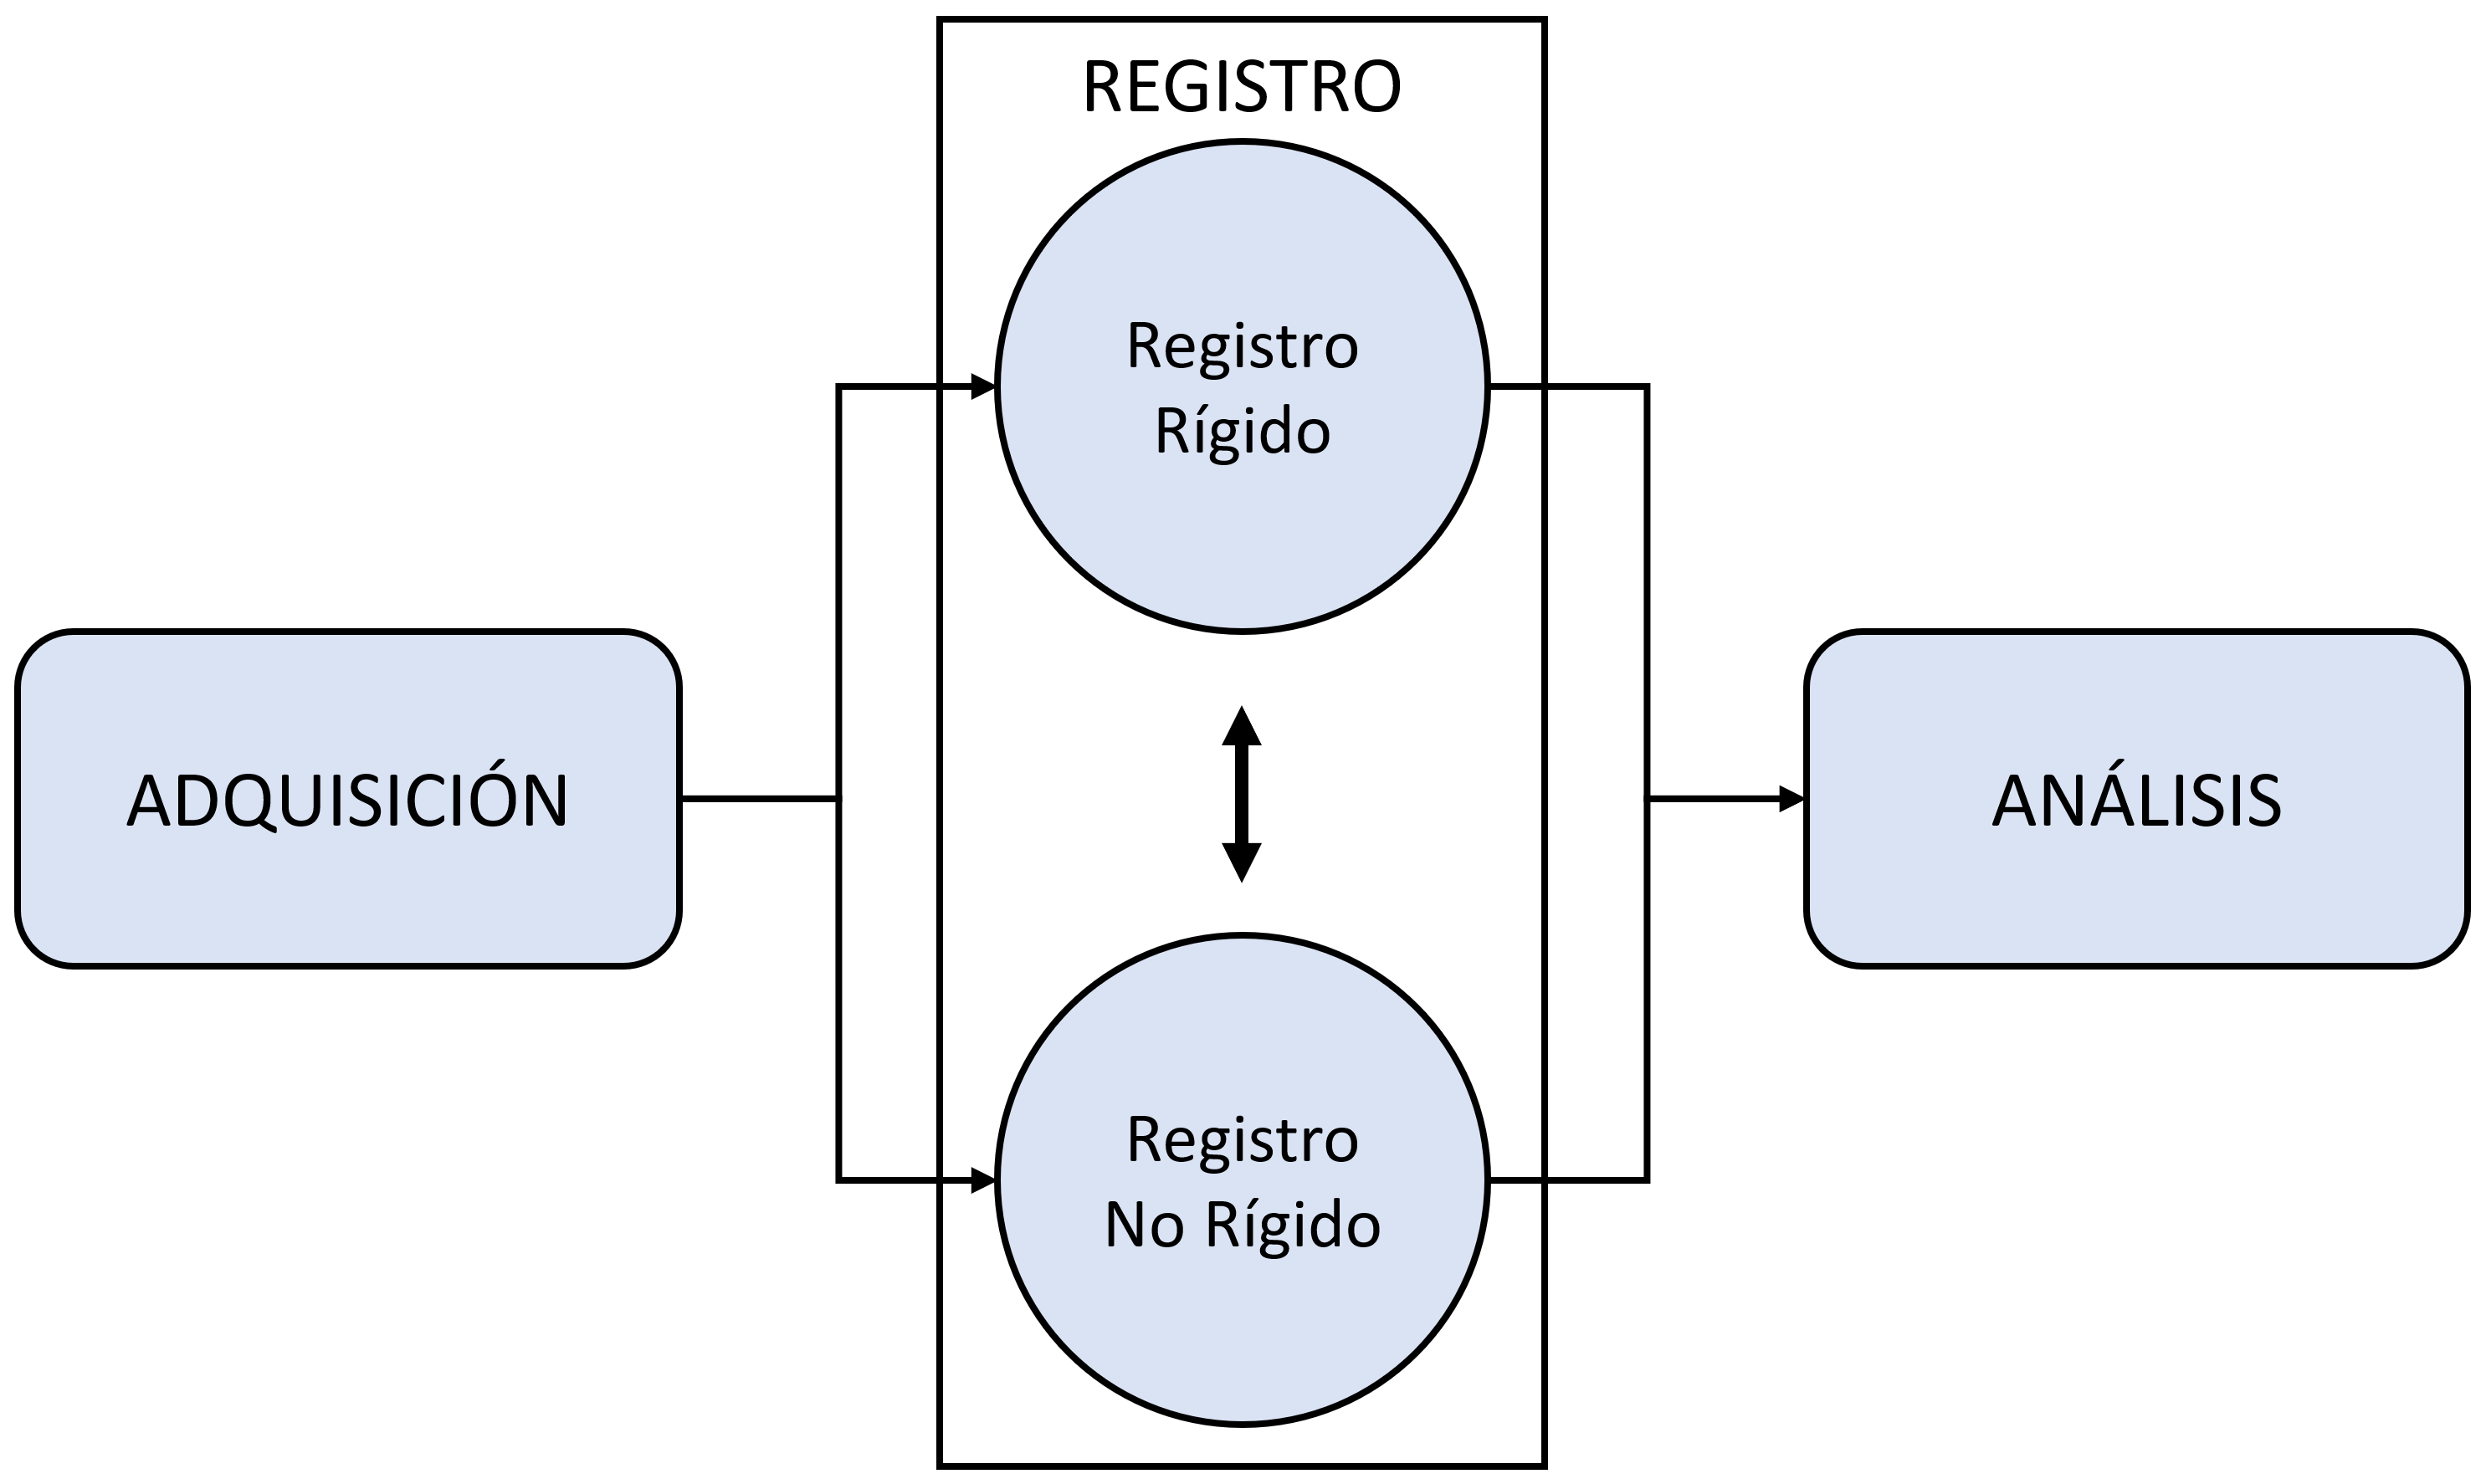
\includegraphics[height=6cm]{archivos/adquisicion-registro-analisis.png}
    \caption{Esquema general de un sistema \glsentryshort{3d}.}
    \label{fig:adquisicion-registro-analisis}
\end{figure}

La adquisición es la primera de las fases para obtener el análisis de una escena.
En esta fase inicial es donde se toman los datos de entrada, por tanto, es la parte del proceso donde interviene el sensor utilizado.
Esta es una parte crítica del sistema, debido a que el resultado de las fases posteriores depende por completo de los datos adquiridos.

% La adquisición de los datos de entrada depende de tres factores principales:
% parámetros del entorno, parámetros del motivo y parámetros de la cámara.
% Los parámetros de entorno hacen referencia al estado en el que se encuentra el entorno, luminosidad, sombras, etc.
% Los parámetros de motivo se refieren a los colores que hay sobre la escena, debido a que el sensor puede estar proyectando colores sobre esta para determinar la profundidad y si coinciden podría dificultar la obtención de los datos.
% Los parámetros de la cámara son los referentes al apartado técnico de la misma:
% la distancia focal, el punto principal, las distorsiones ópticas, el tamaño del sensor, etc.

Tras obtener los datos de entrada en la fase de adquisición, la fase del registro se encarga de realizar las transformaciones necesarias para obtener un modelo completo de la escena.
Existen dos tipos principales de registro:
registro rígido y registro no rígido.
El registro rígido transforma todos los datos al unísono para llevarlos a un mismo sistema de coordenadas, el registro no rígido permite alinear los datos de forma independiente.
Este último es útil para analizar cambios de forma o de color dependiendo del espacio que se esté analizando.

En la última fase, el análisis, se extrae la información necesaria de los datos obtenidos y procesados para cumplir el propósito del problema original.
Este propósito será el que define los requerimientos para la fase de adquisición y de registro.

Por ejemplo, si la escena a analizar se trata de un objeto encima de una mesa, el proceso podría ser obtener los datos desde distintos puntos de vista como primer paso (fase de adquisición).
Seguidamente registrar todas las vistas para que formen el modelo \gls{3d} completo (fase de registro).
Finalmente, el análisis del modelo \gls{3d} nos permite obtener datos útiles de la reconstrucción, como la altura, el volumen, los colores, la forma, etc (fase de análisis).

Habitualmente se asume que los sensores están calibrados para mejorar la adquisición, y el registro de los datos \gls{3d} permita una mejor precisión y exactitud en la fase del análisis.

\section{Estado del arte}
\label{introduccion-estado-arte}

Para abordar este proyecto construyendo un sistema embebido, portable y a la vez económico, se han explorado los diferentes dispositivos que existen en el mercado necesarios para abarcar las diferentes fases del sistema que pretendemos crear.
Es decir, estudiaremos por una parte los diferentes sensores que hay en el mercado para la adquisición de los datos, y por otra parte el hardware necesario que se encargará del registro y del análisis de estos datos.
Además, analizaremos la situación social actual para entender qué necesidades existen y la utilidad que aporta un sistema como el que se pretende construir.
Por último, se hará una pequeña investigación sobre proyectos similares para entender cuál es el estado actual de la tecnología y qué posibilidades ofrece.

\subsection{Hardware para adquisición de datos}
La fase de adquisición depende por completo del sensor utilizado para ello.
Por tanto, es necesario analizar los distintos tipos de sensores para determinar qué sensor será utilizado para dicha finalidad.

% Existen diversos tipos de sensores, y estos se pueden diferenciar principalmente en dos grupos:
% sensores de contacto y sensores sin contacto.

% Los sensores de contacto obtienen la información \gls{3d} de un objeto a través del contacto directo con el mismo.
% Sin embargo, los sensores sin contacto son capaces de obtener esta información desde la distancia.
% Estos últimos suelen ser más rápidos y proporcionan datos adicionales como el color.

Los sensores \gls{3d} pueden diferenciarse en las siguientes categorías:
\gls{lidar}, \gls{tof}, cámaras estereoscópicas y luz estructurada.

\begin{description}
    \item[\gls{lidar}:]
    
    Los sensores \gls{lidar} proyectan un láser en la escena y analizan la reflexión para determinar la distancia y obtener un mapa de profundidad.

    \item[\gls{tof}:]
    
    Los sensores \textit{\glsentrylong{tof}} o ``Tiempo de Vuelo'' en español también proyectan un haz de luz, pero en este caso analizan el tiempo transcurrido entre la emisión y el retorno de dicho haz de luz para determinar la distancia.
    
    A diferencia de los \gls{lidar}, no utilizan un solo pulso de disparo, sino que emiten un cono de disparos, obteniendo información sobre todos los píxeles de la imagen.
    Los escenarios con objetos poco reflectantes pueden tener un impacto negativo en las mediciones realizadas con esta tecnología.
    
    \item[Luz estructurada:]
    
    Los sensores de luz estructurada proyectan un patrón conocido en la escena y calculan la disparidad entre el patrón observado y el conocido.
    Dependiendo del tipo de cámara, puede utilizar patrones codificados temporal o espacialmente.

    Las cámaras de luz estructurada con patrones codificados temporalmente utilizan más de un patrón para crear la imagen y diferenciar los elementos visuales.
    Sin embargo, este enfoque requiere sincronización entre el proyector de patrones y la cámara. 
    
    Por otro lado, las cámaras con patrones codificados espacialmente utilizan similitudes de vecindad espacial y no requieren patrones múltiples.
    No obstante, esta técnica puede presentar problemas en bordes o si hay oclusión del objeto en relación al proyector.

    La iluminación del entorno, así como el motivo, pueden dificultar la identificación del patrón.
    Una vez identificado el patrón, se puede determinar la distancia entre el objeto y la cámara.
    Para ello, es necesario analizar las deformaciones que sufre el patrón sobre la superficie del objeto.

    \item[Cámaras estereoscópicas:]
    
    Las cámaras estereoscópicas consisten en utilizar más de una cámara calibrada en diferentes posiciones para estimar la profundidad calculando la disparidad entre las imágenes obtenidas por cada cámara.

    Se basan en una técnica que utiliza el desplazamiento espacial entre un par de imágenes para triangular y calcular la distancia real entre los objetos y la cámara.
    Muchos sistemas utilizan algoritmos de extracción de características y pueden presentar algunos problemas al intentar identificar puntos clave en escenarios con texturas deficientes.

    A diferencia de los sensores mencionados anteriormente, estos son capaces de proporcionar información de color, pero es necesario calibrar ambos sensores cada vez que varíe su emplazamiento, por tanto, son sensores poco portables.

\end{description}

Los sensores \gls{rgbd} son sensores de propósito general y comúnmente conocidos por su ``bajo coste''.
Combinan las diferentes técnicas de los sensores anteriores con cámaras de color que permiten obtener de forma simultánea la profundidad y el color de la escena.
A través de un sensor \gls{rgbd} podemos obtener un modelo \gls{3d} de un objeto a través de múltiples vistas rotando alrededor del mismo.

En la Figura \ref{fig:d435-sensors} podemos ver un ejemplo de sensor \gls{rgbd}, la Intel RealSense D435.
Este sensor utiliza cámaras estereoscópicas (``Right Imager'' y ``Left Imager'') acompañadas de un proyector \gls{ir} que se encuentra en medio de estas.
El proyector \gls{ir} es una fuente de luz que sirve para iluminar la escena proyectando un patrón de puntos que ayuda a identificar puntos comunes entre las cámaras estereoscópicas.
Estos tres componentes se encargan de capturar la profundidad y están acompañados de un módulo \gls{rgb} para poder capturar la información del color.

\begin{figure}[h]
    \centering
    \begin{subfigure}{0.4\textwidth}
    	\centering
        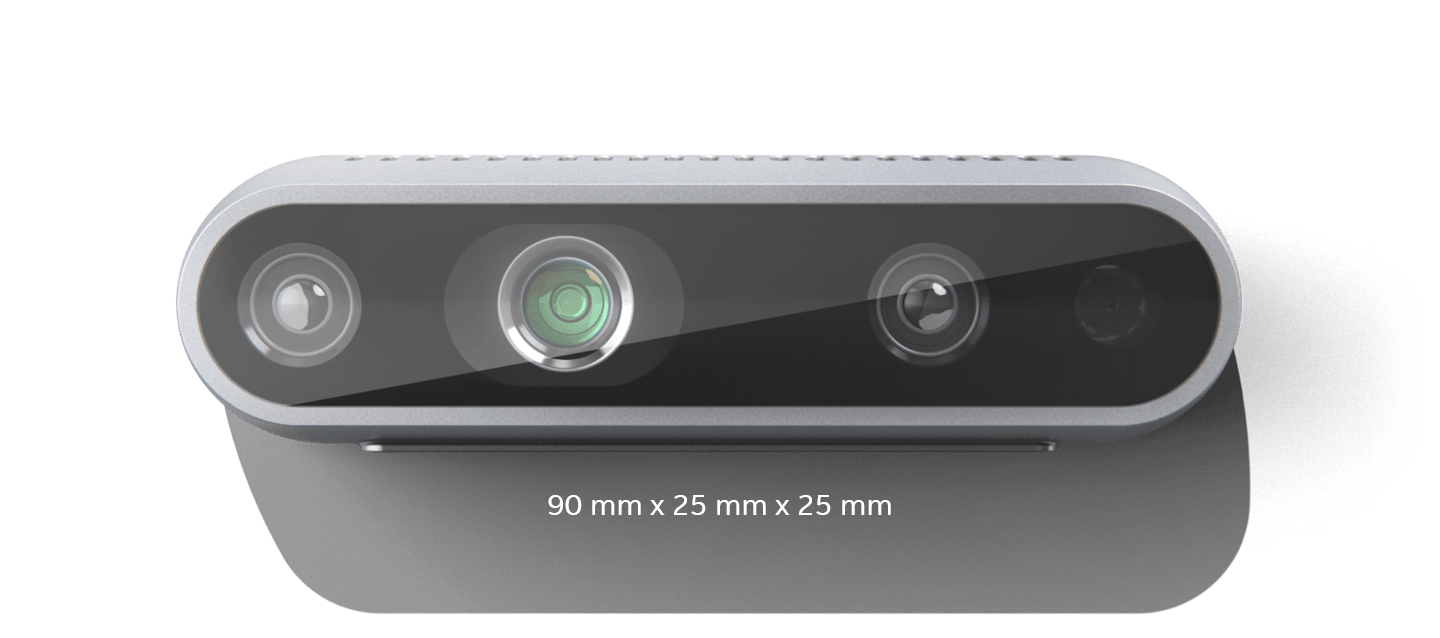
\includegraphics[width=\textwidth]{archivos/d435_image.png}
    \end{subfigure}
    \begin{subfigure}{0.5\textwidth}
    	\centering
        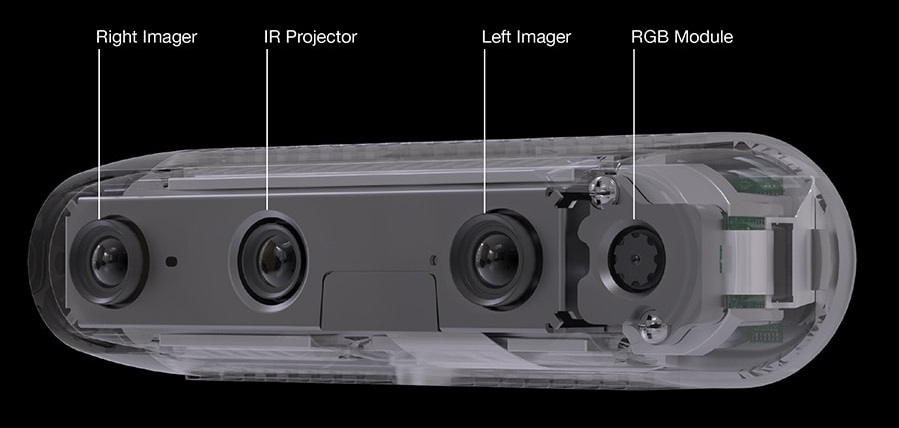
\includegraphics[width=\textwidth]{archivos/d435_sensors.jpg}
    \end{subfigure}
    \caption{Sensor Intel RealSense D435.}
    \label{fig:d435-sensors}
\end{figure}

Como hemos visto, existen diversas categorías de cámaras \gls{3d} con diferentes tecnologías para capturar objetos.
En ``Comparison of RGB-D sensors for 3D reconstruction'' \citep{DaSilvaNeto2020} han realizado una comparación con 10 cámaras \gls{rgbd} de bajo coste distintas para concluir cuáles son las que presentan mejores resultados.

En la Figura \ref{fig:comparacion-sensores-media-error} podemos ver como resultado la media de error obtenida para los 3 recorridos que se han hecho en cada cámara.

\begin{figure}[h]
    \centering
    \begin{subfigure}[b]{0.35\textheight}
    	\centering
        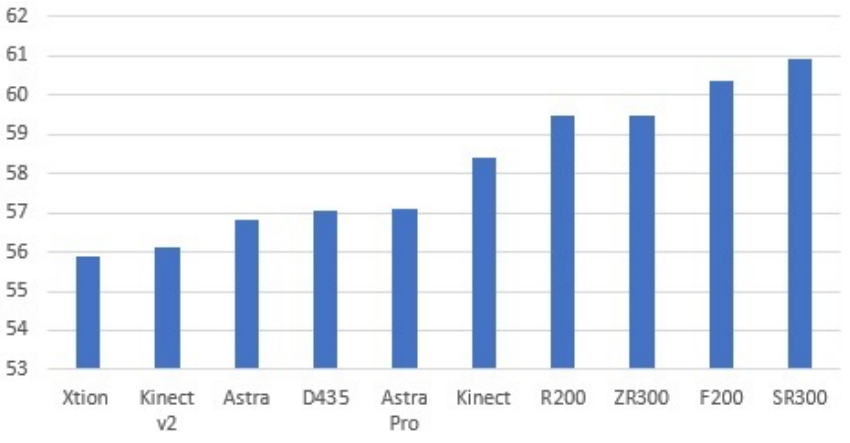
\includegraphics[height=3.5cm]{archivos/comparacion-sensores-recorrido1.png}
        \caption{Ruta 1. Giro simple de 360º.}
        \label{fig:comparacion-ruta1}
    \end{subfigure}
    \begin{subfigure}[b]{0.35\textheight}
    	\centering
        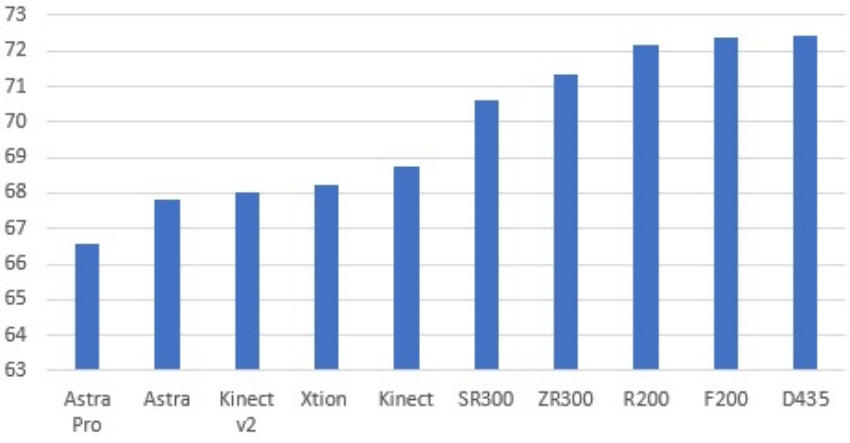
\includegraphics[height=3.5cm]{archivos/comparacion-sensores-recorrido2.png}
        \caption{Ruta 2. Giro de movimiento ondulado.}
        \label{fig:comparacion-ruta2}
    \end{subfigure}
    \begin{subfigure}[b]{0.35\textheight}
    	\centering
        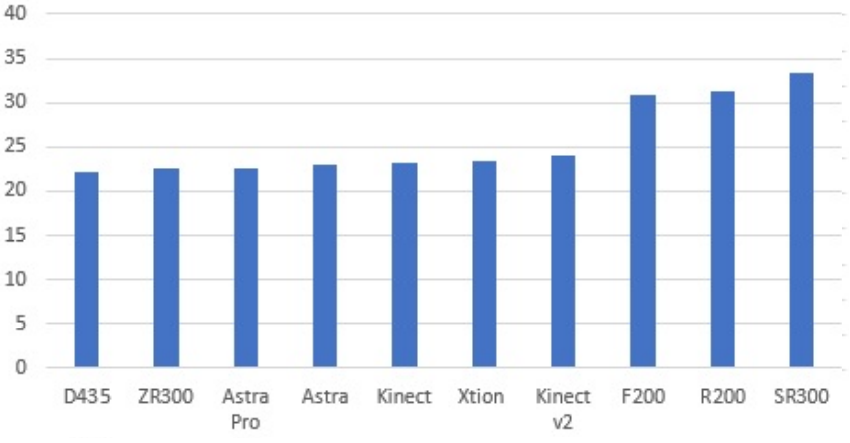
\includegraphics[height=3.5cm]{archivos/comparacion-sensores-recorrido3.png}
        \caption{Ruta 3. Giro cambiando distancia hacia las paredes (acercándose y alejándose).}
        \label{fig:comparacion-ruta3}
    \end{subfigure}
    \caption{Media de error en la comparación de sensores \glsentryshort{rgbd}.}
    \label{fig:comparacion-sensores-media-error}
\end{figure}

% En cada una de las rutas se realiza un giro con la cámara alrededor de la habitación para obtener los datos y recontruirla posteriormente.
% La ruta 1 realiza un giro simple de 360º alrededor de la habitación, la ruta 2 realiza el mismo giro pero con un movimiento ondulado y finalmente la ruta 3 realiza un giro acercandose y alejandose a los objetos.

En general, el Intel D435 obtiene resultados aceptables en las rutas 1 y 3, que son las más similares al caso que abordaremos en este \gls{tfg}.

La prueba donde más destaca el Intel RealSense D435 es en la ruta 3, Figura \ref{fig:comparacion-ruta3}, donde la cámara realiza acercamientos a los objetos.
Esto indica que esta cámara trabaja mejor en escenarios donde la cámara se posiciona cerca del objeto o cuerpo a escanear, lo cual corresponde al objetivo de este \gls{tfg}.

Además, la Intel RealSense D435 se trata del mismo sensor que se utiliza en el proyecto \cite{Tech4DietResultados} del que se ha hablado en la sección \ref{introduccion-motivacion-contexto} de Motivación y Contexto.
Por tanto, este será el sensor a utilizar en este trabajo.

\subsection{Hardware para el registro y análisis de los datos}

Para cumplir con el apartado de registro y análisis de los datos necesitaremos hacer uso de un computador que nos permita:
por una parte almacenar y realizar las modificaciones necesarias a los datos de entrada;
y por otra parte analizar y extraer la información necesaria para el propósito del problema.

Uno de los requisitos que nos proponemos en este proyecto es la capacidad de realizar esto con un dispositivo que sea económico y a la vez portable.
Para ello, se han explorado distintas opciones, como:

\begin{description}
    \item[Raspberry Pi 4 Model B:]
    
    se trata del último modelo de la serie Raspberry Pi. La Raspberry es un mini computador construido en un sistema embebido con un rendimiento comparable con el de un ordenador de sobremesa personal de gama baja.
    
    Estos dispositivos se pueden utilizar como pequeños ordenadores debido a su gran potencial.
    También tiene la capacidad suficiente para usarse como servidor personal por ejemplo.

    Comparado con la anterior generación (Raspberry Pi 3 Model B+) ofrece un aumento significativo en la velocidad del procesador, memoria y conectividad.

    Cuenta con una \gls{cpu} Quad-Core ARM Cortex-A72 de 64 bits a 1.5 GHz de velocidad.
    En cuanto a la \gls{gpu}, cuenta con el chip Broadcom VideoCore VI, con una velocidad de 500 MHz.
    La capacidad de memoria \gls{ram} es de 8 GB LPDDR4 y cuenta con todo tipo de conexiones (USB tipo C, USB Tipo B, microHDMI, conector para cámara\dots).
    
    Con estas especificaciones consigue una potencia computacional de 13.5 GFlops.
    El precio de mercado de este dispositivo está alrededor de 35,00€\footnote{\label{fn:price}El precio indicado se trata del \gls{pvp} oficial recomendado por los fabricantes. Debido a la carencia de chips durante el año 2022 estos precios no se corresponden con la realidad, pudiendo encontrar estos productos por precios mucho más elevados o incluso no quedar stock de los mismos.}.

    \item[Nvidia Jetson Nano:]
    
    la Jetson Nano es la gama de entrada de la familia de Nvidia Jetson.
    Nvidia Jetson es una serie de computadores embebidos, parecidas a las Raspberrys pero con \gls{gpu}s más potentes.
    Esto nos permitirá realizar operaciones en paralelo en algoritmos para la visión por computador.

    Cuenta con una \gls{cpu} Quad-Core ARM Cortex-A57 de 64 bits a 1.42 GHz de velocidad.
    En cuanto a la \gls{gpu}, el chip está basado en la arquitectura Maxwell de Nvidia, cuenta con 128 \gls{cuda} cores con una velocidad de 921 MHz.
    La capacidad de memoria \gls{ram} es de 4 GB LPDDR4 y cuenta con todo tipo de conexiones (USB tipo C, USB Tipo B, microHDMI, conector para cámara\dots).

    Con estas especificaciones consigue una potencia computacional de 472 GFlops.
    El precio de mercado de este dispositivo está alrededor de 89,00€\footref{fn:price}.

    \item[Nvidia Jetson TX2:]
    
    se trata de un modelo superior a la Jetson Nano, con especificaciones superiores, pero también más caro.

    Cuenta con una \gls{cpu} Quad-Core ARM Cortex-A57 de 64 bits a 2.00 GHz de velocidad.
    En cuanto a la \gls{gpu}, el chip está basado en la arquitectura Pascal de Nvidia, cuenta con 256 \gls{cuda} cores con una velocidad de 1300 MHz.
    La capacidad de memoria \gls{ram} es de 8 GB LPDDR4 y cuenta con todo tipo de conexiones (USB tipo C, USB Tipo B, microHDMI, conector para cámara\dots).

    Con estas especificaciones consigue una potencia computacional de 1.3 TFlops.
    El precio de mercado de este dispositivo está alrededor de 399,00€\footref{fn:price}.
\end{description}

Como podemos observar, la Nvidia Jetson Nano cuenta con un procesador ligeramente inferior al de la Raspberry Pi 4 Model B.
Sin embargo, la \gls{gpu} es mucho más potente, con 128 núcleos a 921 MHz que permite superar en potencia computacional a la Raspberry unas 35 veces.

Además, nuestro proyecto trabaja con la visión por computadores, lo cual quiere decir que se realizará un gran número de operaciones y cálculos fácilmente paralelizables.
Para poder sacar mejor rendimiento y aprovechar la concurrencia de los cálculos, viene bien hacer uso de una \gls{gpu} con muchos núcleos, por tanto será necesario una \gls{gpu} más potente que el chip que incluye la Raspberry Pi 4 Model B.

Por otro lado, la Nvidia Jetson TX2 es claramente superior en especificaciones a la Nvidia Jetson Nano.
Cuenta con un procesador un poco más potente y una \gls{gpu} con el doble de núcleos a 1300 MHz de velocidad, superando en potencia computacional casi 3 veces a la Jetson Nano, pero con un precio muy superior.

``Benchmark Analysis of Jetson TX2, Jetson Nano and Raspberry PI using Deep-CNN''
\citep{Suzen2020} se trata de una investigación donde miden el rendimiento de estos tres dispositivos para aplicaciones que usan deep learning. Si bien nuestro proyecto de investigación no se basa en el deep learning, el principio para determinar el rendimiento de estos dispositivos es el mismo, la concurrencia.

En el estudio de \cite{Suzen2020} utilizan 5 conjuntos de datos de varios tamaños.
En la Figura \ref{fig:resultados-benchmark-tx2-nano-raspberry} se ve que hay un error de memoria para la Nvidia Jetson Nano y la Raspberry Pi.
No es un problema que deba preocuparnos ya que esto es un problema que surge cuando se requiere de un conjunto tan grande de datos para el deep learning.
Para nuestro proyecto, basado en la visión por computador, no será un límite a tener en cuenta.

También podemos ver el resultado del estudio, con el porcentaje de aciertos, el tiempo que emplean, la memoria utilizada y el consumo.
Para nuestro caso, el resultado de mayor interés a tener en cuenta es el tiempo, ya que es la forma de medir qué dispositivo tiene un mejor rendimiento.

\begin{figure}[h]
    \centering
    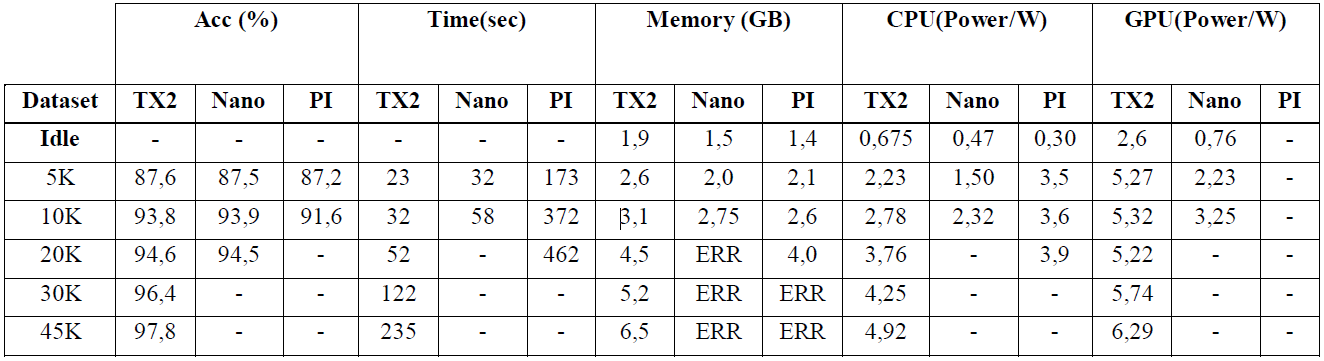
\includegraphics[width=\linewidth]{archivos/resultados-benchmark-tx2-nano-raspberry.png}
    \caption{Benchmarking Nvidia Jetson TX2, Nvidia Jetson Nano y Raspberry Pi 4 Model B.}
    \label{fig:resultados-benchmark-tx2-nano-raspberry}
\end{figure}

Como podemos ver, las Nvidia Jetson quedan muy por encima de la Raspberry Pi 4 Model B, con unos resultados muy parecidos entre ellas, siendo superior la Nvidia Jetson TX2 en todos los casos.

Aunque la Nvidia Jetson TX2 es la clara ganadora en rendimiento, para este proyecto la potencia no lo es todo.
Entre nuestros requisitos para construir el escáner \gls{3d}, los dispositivos a utilizar deben ser portables y económicos. Los 3 computadores que hemos comparado son igual de portables, pero la Jetson TX2 tiene un precio demasiado elevado para el coste económico que estamos buscando.

Para poder comparar la calidad/precio de cada uno de los dispositivos, nos fijaremos en la potencia computacional para medir la calidad de los mismos.
Por tanto, nos centraremos en el precio del GFlop en cada uno de los dispositivos.
Podemos ver que en la Raspberry Pi 4 Model B tendría un coste de 2,60€/GFlop, la Nvidia Jetson Nano un coste de 0,19€/GFlop y la Nvidia Jetson TX2 un coste de 0,30€/GFlop.

Además, si nos basamos en los resultados de los benchmarks que se muestran en la Figura \ref{fig:resultados-benchmark-tx2-nano-raspberry}, la diferencia de rendimiento en tiempo entre la Nvidia Jetson Nano y la Nvidia Jetson TX2 no es tan grande como para compensar el coste económico que supone hacerse con una Nvidia Jetson TX2.

Por tanto, la opción más recomendable para este proyecto es, sin lugar a dudas, la Nvidia Jetson Nano, que nos ofrece un rendimiento aceptable, muy superior a una Raspberry PI y por un precio muy económico.

% No obstante, hay que tener en cuenta que no es comparable el rendimiento que estos computadores embebidos pueden proporcionar frente a sobremesas que cuentan con una \gls{gpu} dedicada.

% Como podemos ver en ``Benchmarking GPU-Accelerated Edge Devices'' \citep{Jo2020}, otro estudio sobre el uso de \gls{gpu} para deep learning, las Nvidia Jetson Nano y TX2 son capaces de completar los benchmarks eficientemente.
% No obstante, no son comparables con el rendimiento de \gls{gpu}s como la GTX 1060 o la Tesla V100, gráficas dedicadas que han utilizado en los benchmarks de la investigación.
% En estos benchmarks se demuestra que para procesos o aplicaciones demasiado complejas los computadores embebidos pueden ser insuficientes.

% Para el propósito de este proyecto, el rendimiento que nos proporcionará la Nvidia Jetson Nano es suficiente.

\subsection{Situación social actual, necesidades y aplicaciones}

Un escáner \gls{3d} tiene la capacidad de analizar un objeto o una escena para reunir datos sobre su forma y, ocasionalmente, su color.
Con la información obtenida se puede pasar a construir modelos digitales tridimensionales.

Al principio, las utilidades y aplicaciones que proporcionaba esta tecnología era utilizada exclusivamente en el ámbito industrial.
Hoy en día, gracias a los avances y a la popularidad de la tecnología, es utilizada en una amplia variedad de actividades, tales como arquitectura, ingeniería, medicina, arqueología y entretenimiento, entre otras.
A continuación, comentaré algunos ejemplos de ellos. Veremos como son muchas las utilidades que un escáner \gls{3d} ofrece, y que existe la necesidad de herramientas así que sean portables y de bajo coste.

En el ámbito industrial e ingenieril tiene diferentes aplicaciones debido a su gran capacidad para capturar de forma rápida y precisa los datos requeridos.
De otra forma, las mediciones tendrían que ser recolectadas por métodos manuales que pueden ser menos exactos, muy costosos y consumir mucho tiempo.
Como por ejemplo se estudia en el artículo ``Generación de prototipos por modelado, escaneado e impresión 3D'' \citep{RayonEncinas2015} de la \gls{upv} donde desarrollan una metodología docente enfocada a los alumnos de \gls{ididp} para el uso del escáner \gls{3d}. En este informe dan a conocer la importancia y necesidad del escáner \gls{3d}, donde digitalizan un objeto en \gls{3d} y realizan modificaciones en el diseño para finalmente generar un prototipo real por impresión \gls{3d}, facilitando así el desarrollo de un producto.

En el ámbito de la salud más cercano a la temática del proyecto los requerimientos de escaneo \gls{3d} son diversos, como explican en el artículo científico ``3D scanning applications in medical field: A literature-based review'' \citep{Haleem2019} donde hablan de la importancia de esta tecnología y del crecimiento que ha tenido en el campo de la medicina en los últimos años.
Por ejemplo, los profesionales de la salud pueden de forma muy rápida realizar un escaneo corporal completo, facilitando así la obtención y comparación de datos precisos para llevar a cabo investigaciones y monitorizar los cambios en las mediciones corporales que ocurren con el tiempo.
Esto es posible gracias a investigaciones como las que se han hecho en \cite{Tech4DietResultados}, con artículos científicos como ``RGB-D-Based Framework to Acquire, Visualize and Measure the Human Body for Dietetic Treatments'' \citep{Fuster-Guillo2020}.

Por otro lado, el escaneo \gls{3d} también trae la posibilidad de crear soluciones personalizadas para el cuidado de la salud.
Por ejemplo, en ``Reconstrucción digital del muñón de un amputado transfemoral a partir de datos obtenidos de escáner 3D'' \citep{isaza2011reconstruccion} muestran como el uso de un escáner \gls{3d} permite realizar reconstrucciones sobre un molde tomado de un muñón.
``Diseño de prótesis inferiores impresas en 3D para personas amputadas en Camerún'' \citep{martinez2020diseno} es otro ejemplo donde muestran el desarrollo del proceso de diseño de prótesis inferiores, haciendo uso de técnicas de digitalización e impresión \gls{3d}, debido a que es rápida, económica y permite la personalización de las prótesis para cada paciente.

En el ámbito de la medicina forense también se está experimentando un crecimiento en el uso de técnicas \gls{3d}.
Ofrecen portabilidad, flexibilidad y precisión que facilita la tarea de recopilar datos forenses comparado con los métodos tradicionales.
Por ejemplo, en la investigación ``Geotecnologías láser y fotogramétricas aplicadas a la modelización 3D de escenarios complejos en infografía forense'' \citep{blazquez2015geotecnologias} proponen el uso de escáneres \gls{3d} para la identificación por superposición craneofacial.
Para ello, utilizan una plataforma giratoria que automatiza la adquisición de las distintas vistas del cráneo para aumentar la rapidez y precisión de la obtención del modelo \gls{3d}.
Un concepto muy parecido al que se desea realizar en este trabajo.

Por último, en el ámbito de la paleontología y arqueología gracias a las tecnologías \gls{3d} se ha conseguido la creación de réplicas digitales de gran precisión de diversos artefactos, desde la recreación de elementos encontrados durante excavaciones hasta la creación de museos online con cientos de exhibiciones.
En ``Restauración y conservación digital de fósiles mediante escaneado 3D y la reproducción con prototipado rápido'' \citep{Valverde-Bastidas2020} se utiliza ingeniería inversa mediante el escaneado \gls{3d} para obtener una nube de puntos en tres dimensiones de un objeto material.
Posteriormente tratan esa malla para luego realizar una reingeniería, un rediseño o directamente para volver a fabricar el objeto.

\subsection{Investigaciones y otros proyectos ya realizados}

Se han investigado proyectos cuyo hardware es parecido al que se pretende utilizar en este trabajo de investigación.
En ``Analysis of 3D perception based on depth sensors in order to perform 3D scene understanding'' \citep{fioriti2021analysis} pretenden realizar un análisis de las características de percepción 3D con la ayuda de sensores de profundidad.
Para ello han utilizado una cámara \gls{rgbd} Intel RealSense D435 conectada inicialmente a una Raspberry Pi 3, utilizando el algoritmo de detección Yolo adaptado para usar una detección \gls{3d}.
De esta forma, han implementado un sistema capaz de detectar la distancia que hay con el objeto.
El algoritmo puede ser utilizado tanto con imágenes como con un vídeo del objeto.
El problema actual que tienen es que no puede ser utilizado en tiempo real, pues para ello necesitan acelerar el proceso.
Esto es debido seguramente a las bajas prestaciones del hardware, ya que utilizan una Raspberry Pi 3 cuya \gls{gpu} es muy pobre comparada con la \gls{gpu} de la Nvidia Jetson Nano que utilizaremos en este proyecto.

En ``Development of augmented reality systems displaying three-dimensional
dynamic motion in real time'' \citep{Aoki2020} han utilizado también el sensor D435 conectado a un dispositivo Raspberry Pi 4.
Con este hardware pretenden desarrollar un sistema de seguimiento de un movimiento tridimensional mostrando en tiempo real la trayectoria en un dispositivo móvil.
Por tanto, han desarrollado una aplicación para poder seguir objetos \gls{3d} con el sensor y mostrar la trayectoria en realidad aumentada desde el dispositivo móvil.
Esta aplicación tiene una limitación respecto a la velocidad del movimiento, ya que la frecuencia del muestreo ha sido limitada a 8 fps debido a las especificaciones del hardware.
De nuevo, esto se podría solucionar utilizando un hardware más potente como la Nvidia Jetson Nano, que permitiría paralelizar gran parte del proceso aumentando la frecuencia del muestreo máxima y permitiendo así detectar movimientos más rápidos.

\section{Objetivos}
\label{introduccion-objetivos}

El objetivo general es proponer una arquitectura de visión por computador que sea capaz de modelar en \gls{3d} objetos deformables. Concretamente, para este \gls{tfg} el objetivo principal es hacer un sistema embebido de bajo coste que permita modelar un cuerpo o individuo articulado, como lo es un cuerpo humano.
Para ello, se plantean tres subobjetivos:

\begin{itemize}
    \item El primer subobjetivo es realizar un análisis del estado del arte para evaluar la situación en la que nos encontramos. Además, se analizarán las tecnologías y herramientas necesarias para llevar a cabo el objetivo del proyecto.
    \item Hacer una propuesta de solución. Este subobjetivo consistirá en integrar el SDK del sensor \gls{rgbd} Intel RealSense D435 con el dispositivo Nvidia Jetson Nano, implementar una solución, validarla y documentarla.
    \item Por último, experimentar y estudiar los resultados obtenidos.
\end{itemize}

\section{Desarrollo de la memoria}
\label{introduccion-desarrollo}

A continuación, los siguientes capítulos contendrán las bases teóricas y el desarrollo del tema principal del trabajo.
Está organizado de la siguiente manera:

El capítulo \ref{cap:base-teorica} nos presenta la base teórica necesaria para comprender el desarrollo e investigación que se ha llevado a cabo a lo largo del proyecto.

El capítulo \ref{cap:realsense-d435} habla del sensor Intel RealSense Depth Camera D435.
En este capítulo se analiza más detalladamente el funcionamiento y las características de este sensor, que es el utilizado en este trabajo.

El capítulo \ref{cap:propuesta-de-solucion} muestra la propuesta del trabajo, explicando detalladamente los pasos que se van a seguir para obtener una solución a la reconstrucción de un cuerpo humano utilizando el sensor Intel RealSense D435 y el sistema embebido Jetson Nano.

En el capítulo \ref{cap:solucion-proyecto} explica cómo se ha llevado a cabo la propuesta del capítulo anterior, mostrando fragmentos de código y la solución final obtenida.

Seguidamente en el capítulo \ref{cap:experimentacion} se mostrarán los resultados que se obtienen con la solución del proyecto.

Finalmente, en el capítulo \ref{cap:conclusion} nos encontraremos con la conclusión del trabajo elaborado en este proyecto.

\chapter{Base teórica}
\label{cap:base-teorica}

La reconstrucción de cuerpos u objetos en 3D a partir de un sensor RGBD se consigue gracias al uso de métodos de registro que realizan cálculos de correspondencias entre dos vistas distintas.
Es decir, dado un conjunto de datos de entrada, donde cada entrada son capturas de nubes de puntos de un mismo cuerpo realizadas desde distintos ángulos, el método de registro se encargará de encontrar una transformación que alinee estas nubes de puntos para finalmente reconstruir el cuerpo entero.
Esta transformación no es más que una combinación de rotaciones y traslaciones en los ejes de coordenadas $\mathbf{X}$, $\mathbf{Y}$, $\mathbf{Z}$ sobre la nube de puntos.

\section{Métodos de registro}
\label{sec:metodos-de-registro}

Los métodos de registro tratan de encontrar una correspondencia entre la posición de los puntos de una nube de puntos y otra, emparejándolos para calcular de esta forma la transformación global que corresponda de mejor manera entre los dos conjuntos de nube de puntos.
Estos métodos realizan cálculos en ocasiones de forma iterativa, para encontrar la mejor correspondencia entre los puntos y así estimar la transformación que consiga alinear ambas vistas.

\begin{figure}[h]
    \centering
    \begin{subfigure}[t]{0.33\textheight}
    	\centering
        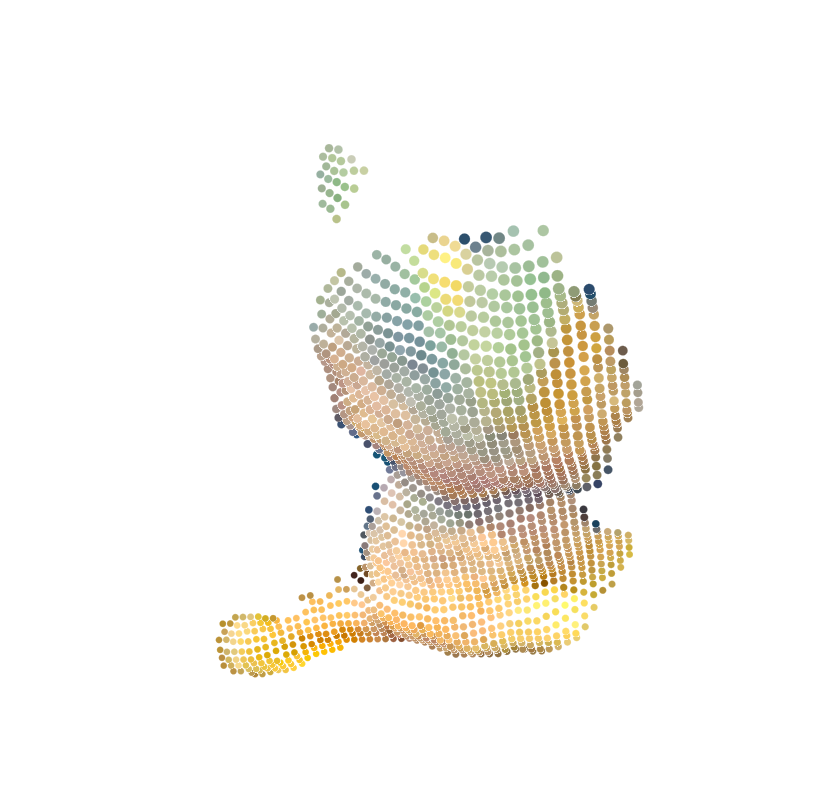
\includegraphics[height=4cm]{archivos/metodo-registro-explicacion-modelo-2.png}
        \caption{Captura del modelo.}
        \label{fig:metodo-registro-explicacion-modelo}
    \end{subfigure}
    \begin{subfigure}[t]{0.33\textheight}
    	\centering
        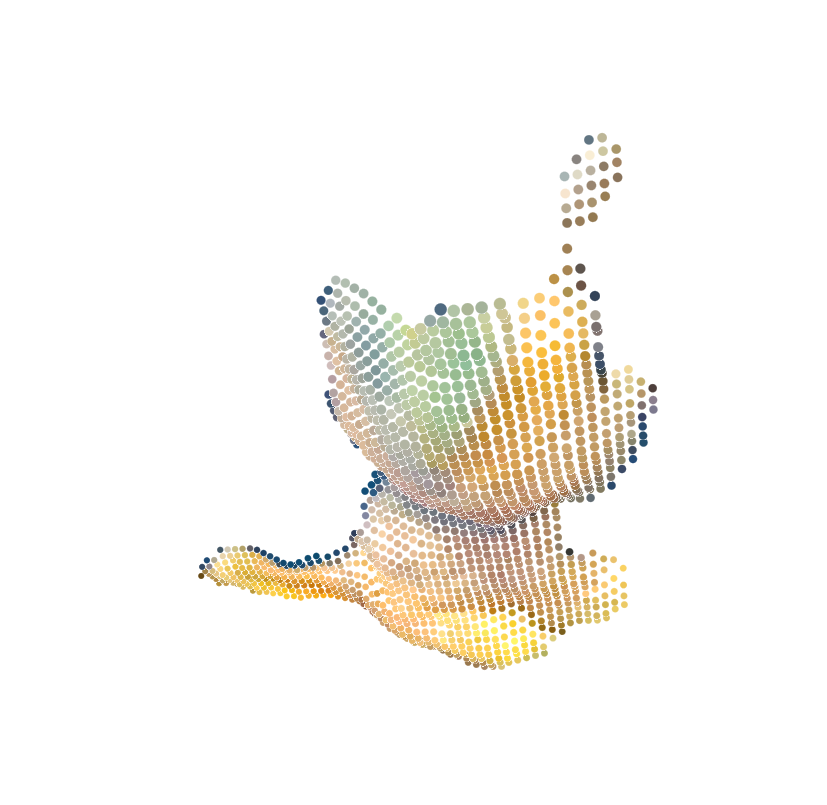
\includegraphics[height=4cm]{archivos/metodo-registro-explicacion-escena-2.png}
        \caption{Captura de la escena.}
        \label{fig:metodo-registro-explicacion-escena}
    \end{subfigure}
    \begin{subfigure}[t]{0.33\textheight}
    	\centering
        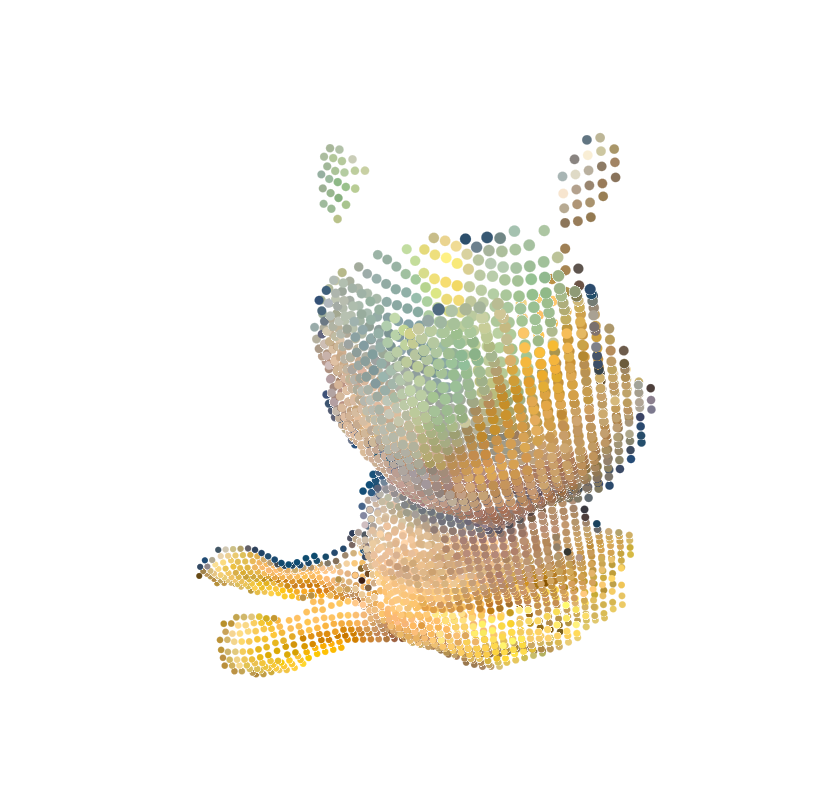
\includegraphics[height=4cm]{archivos/metodo-registro-explicacion-superpuesto-2.png}
        \caption{Modelo y escena superpuestos.}
        \label{fig:metodo-registro-explicacion-superpuesto}
    \end{subfigure}
    \begin{subfigure}[t]{0.33\textheight}
    	\centering
        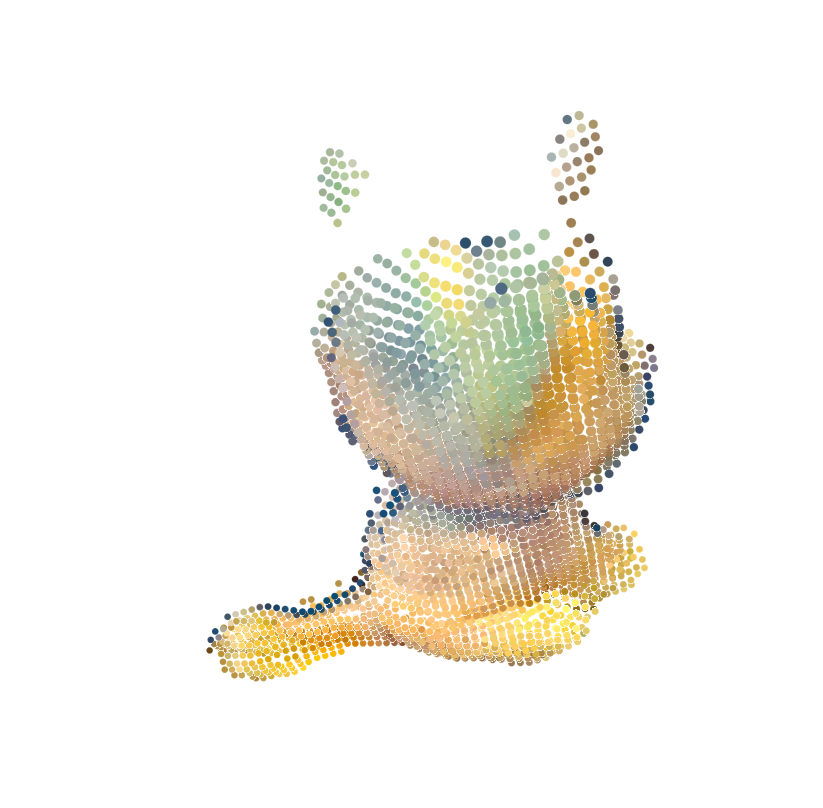
\includegraphics[height=4cm]{archivos/metodo-registro-explicacion-alineacion-2.png}
        \caption{Escena alineada con el modelo.}
        \label{fig:metodo-registro-explicacion-alineacion}
    \end{subfigure}
    \caption{Ejemplo de alineación de una escena con un modelo.}
    \label{fig:metodo-registro-explicacion}
\end{figure}

Como podemos ver en la Figura \ref{fig:metodo-registro-explicacion}, dado dos entradas de nubes de punto, el modelo y la escena, obtenemos su alineación a través de un método de registro.
Normalmente a la nube de puntos de referencia con la que se tratará de alinear el resto de nubes de puntos recibe el nombre de modelo.
Las nubes de puntos que se tratan de emparejar reciben el nombre de escena.
Cuando aplicamos un método de registro sobre una escena (Figura \ref{fig:metodo-registro-explicacion-escena}) y tomamos como referencia un modelo (Figura \ref{fig:metodo-registro-explicacion-modelo}) lo que conseguiremos es transformar la escena para que quede alineada y así forme parte del modelo (Figura \ref{fig:metodo-registro-explicacion-alineacion}).
De esta forma, gracias a la alineación de la escena sobre el modelo, conseguimos que el modelo quede más completo.

\begin{figure}[h]
    \centering
    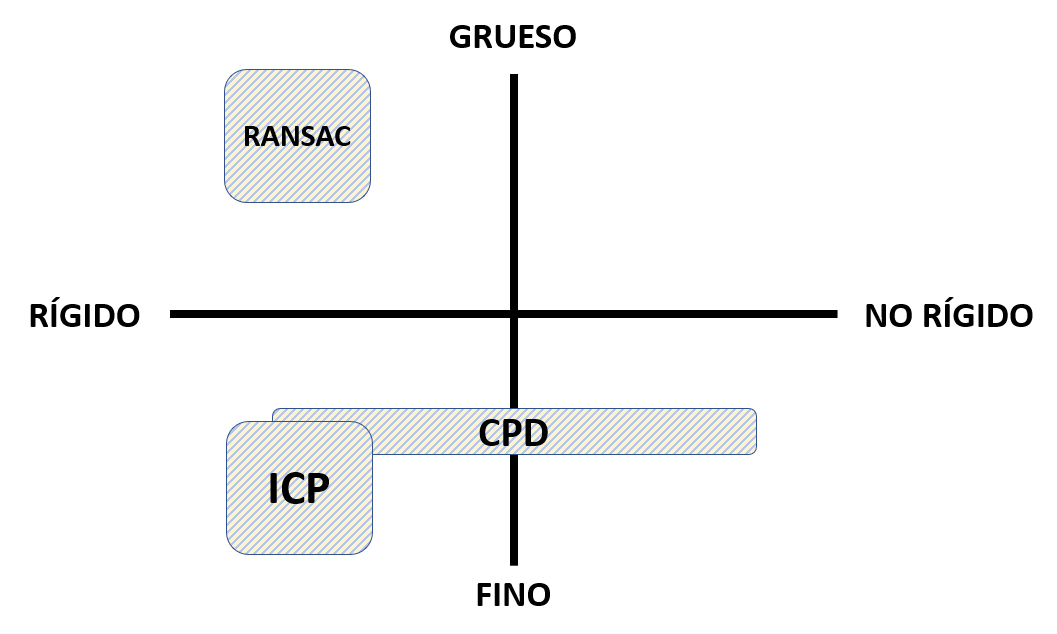
\includegraphics[height=6cm]{archivos/diagrama-tipos-registro.png}
    \caption{Diagrama tipos de registro.}
    \label{fig:diagrama-tipos-registro}
\end{figure}

En la Figura \ref{fig:diagrama-tipos-registro} podemos ver un diagrama que sitúa algunos de los métodos de registros de los que hablaremos en este \gls{tfg} en función de sus características.
Podemos ver que un método de registro se puede diferenciar por ser de grano grueso o grano fino, y por el tipo de registro que se está utilizando para alinear los datos: rígido o no rígido.
    
Los métodos de grano grueso suelen utilizarse como paso inicial en el registro debido a que suelen ser poco precisos, pero ofrecen una buena aproximación inicial para vistas muy separadas entre sí.
Estos métodos suelen muestrear los datos y utilizan métodos basados en detección y descripción de características para intentar reducir la cantidad de puntos tanto de la escena como del modelo.
Una característica (keypoint) tiene una posición y un descriptor que describe
ese keypoint.
Las características proceden de la captura en sí ya sea una imagen \gls{2d} o una nube de puntos (imagen \gls{3d}).
En este paso de detección de características se intenta detectar las partes distintivas de un objeto en los conjuntos de datos, como formas, regiones cerradas, contornos, líneas, etc.
Una vez detectadas las partes del objeto se representa como un conjunto de valores normalmente llamados descriptores de
características.
Tras la detección y descripción de características, se buscan correspondencias entre las mismas y finalmente una estimación de la transformación.

El método basado en características más utilizado para encontrar la transformación entre correspondencias está basado en el paradigma \gls{ransac}, publicado por primera vez por \cite{Fischler1981}.
\gls{ransac} es un método iterativo para calcular los parámetros de un modelo matemático de un conjunto de datos observados que contiene valores atípicos.
Es un algoritmo no determinista en el sentido de que produce un resultado razonable solo con una cierta probabilidad, mayor a medida que se permiten más iteraciones.
En cada iteración del algoritmo, se selecciona aleatoriamente un subconjunto de correspondencias a los que se les aplica una matriz de transformación.
Los datos restantes se testean con el modelo aplicado de manera que si su error está por encima de un umbral se eliminan de los datos seleccionados, de esta forma se descartan los puntos con errores extremadamente altos (outliers).
En la Figura \ref{fig:ransac-ejemplo} podemos ver un ejemplo de alineación con imágenes \gls{2d} utilizando \gls{ransac}.
En la subfigura \ref{fig:ransac-ejemplo-alineado-bien} podemos ver un ejemplo de resultado de una iteración que ha tenido buena probabilidad con la correspondencia entre el subconjunto de puntos seleccionados (subfigura \ref{fig:ransac-ejemplo-correspondencias}).
En la subfigura \ref{fig:ransac-ejemplo-alineado-mal} podemos ver un ejemplo de una iteración que ha partido de una mala correspondencia entre los subconjuntos de los puntos seleccionados.
Este proceso se repite varias veces, finalmente se utilizará la iteración que mejor solución presente como aproximación inicial para un método de registro de grano fino.

\begin{figure}[h!]
    \centering
    \begin{subfigure}[t]{0.5\textheight}
        \centering
        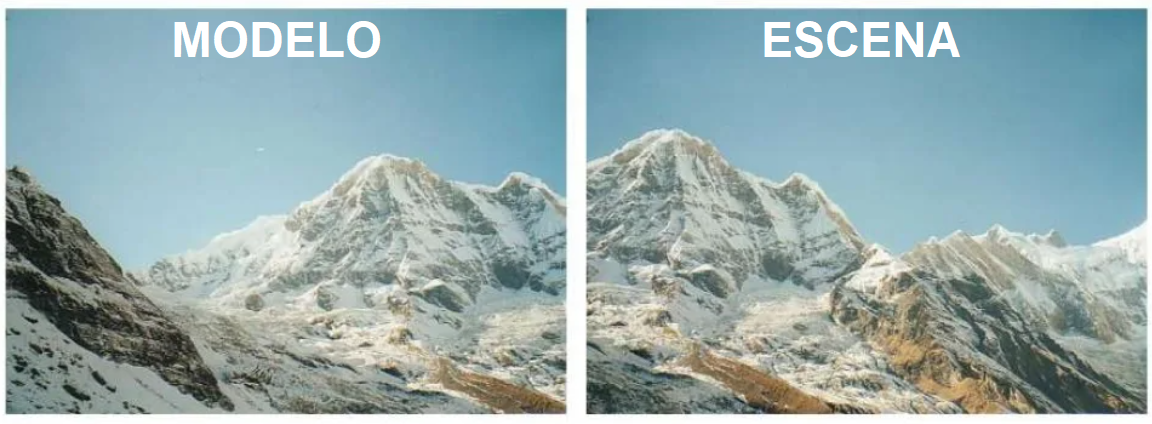
\includegraphics[height=3cm]{archivos/ransac-ejemplo.png}
        \caption{Dos capturas en 2D.}
        \label{fig:ransac-ejemplo-capturas}
    \end{subfigure}
    \begin{subfigure}[t]{0.5\textheight}
        \centering
        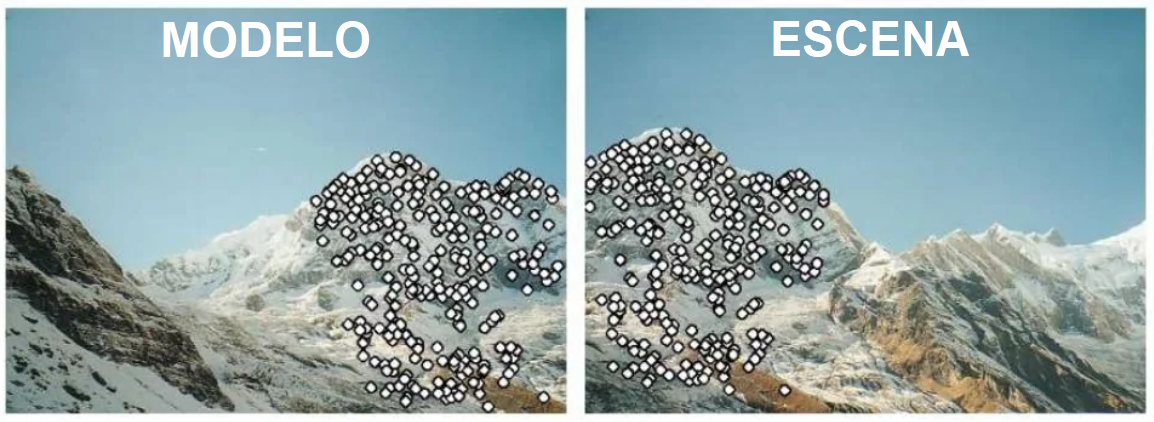
\includegraphics[height=3cm]{archivos/ransac-ejemplo-caracteristicas.png}
        \caption{Búsqueda de características en las capturas.}
        \label{fig:ransac-ejemplo-caracteristicas}
    \end{subfigure}
    \begin{subfigure}[t]{0.5\textheight}
        \centering
        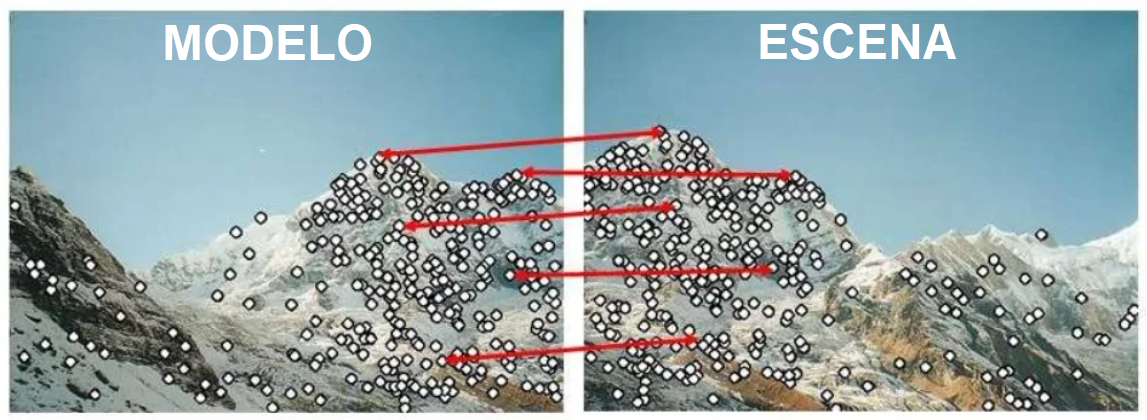
\includegraphics[height=3cm]{archivos/ransac-ejemplo-correspondencias.png}
        \caption{Búsqueda de correspondencias en las capturas.}
        \label{fig:ransac-ejemplo-correspondencias}
    \end{subfigure}
    \begin{subfigure}[t]{0.33\textheight}
        \centering
        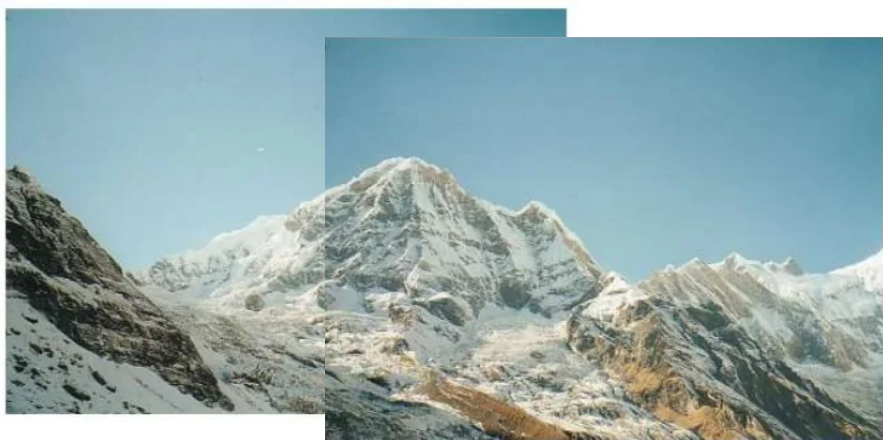
\includegraphics[height=3.5cm]{archivos/ransac-ejemplo-alineado-bien.png}
        \caption{Ejemplo de alineación con correspondencias muy buenas.}
        \label{fig:ransac-ejemplo-alineado-bien}
    \end{subfigure}
    \begin{subfigure}[t]{0.33\textheight}
        \centering
        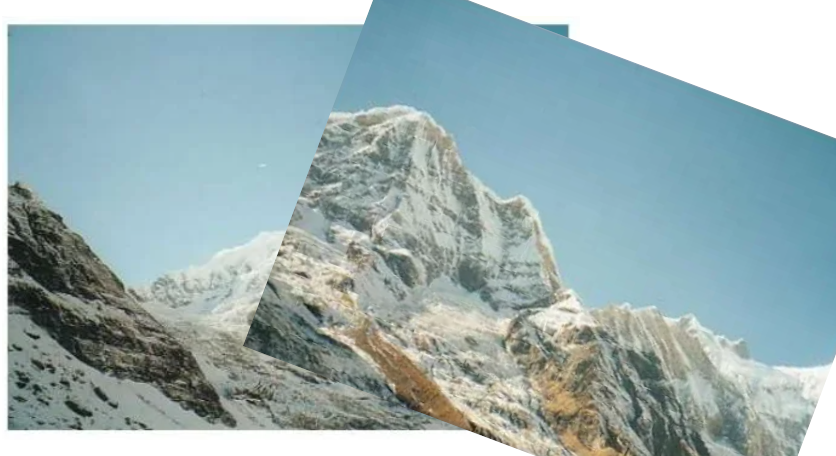
\includegraphics[height=3.5cm]{archivos/ransac-ejemplo-alineado-mal.png}
        \caption{Ejemplo de alineación con correspondencias muy malas.}
        \label{fig:ransac-ejemplo-alineado-mal}
    \end{subfigure}
    \caption{Ejemplo de alineación de una escena usando RANSAC.}
    \label{fig:ransac-ejemplo}
\end{figure}

Los métodos de grano fino se usan normalmente cuando se necesitan resultados más precisos.
Por lo general, estos métodos necesitan el resultado de un registro de grano grueso previo como dato inicial del que partir.
Cuando se le aplica el resultado de un método de grano grueso a la escena, esta se encontrará más próxima al modelo, facilitando así la ejecución de un método de grano fino.
Sin embargo, no siempre es necesario una alineación previa si las nubes de puntos que se intentan alinear ya están lo suficientemente cerca.
Por ejemplo, cuando se usa una frecuencia de capturación en el sensor muy alta, y el movimiento entre dos capturas consecutivas es muy pequeño. 

Como conclusión entre los métodos de grano grueso y fino, los métodos de registro fino se suele utilizar para refinar un registro en el
que la escena y el modelo se encuentran muy próximos, en contraste con los métodos de grano grueso que se suelen utilizar para distancias mayores con la finalidad de aproximar la escena al modelo sin ser del todo preciso.

Por otra parte, los métodos de registro también se pueden diferenciar entre métodos de registro rígidos y métodos de registro no rígidos.
Cuando hablamos de un objeto o cuerpo no rígido, nos referimos a un objeto o cuerpo articulado o deformable.
El registro rígido se utiliza cuando la diferencia entre modelo y escena consiste en una matriz de transformación, es decir, la escena sobre el objeto se ha rotado o movido respecto al modelo sobre el objeto, pero en ambos casos el objeto es el mismo y mantiene la misma forma.
Cuando hablamos de un registro no rígido es porque el objeto de la escena puede haber sido deformado, además de rotado o movido respecto al modelo.

\subsection{Métodos de registro rígidos, ICP}

El método de registro rígido más utilizado es el \gls{icp} \cite{Besl1992}. Es un método de propósito general, independiente de la representación y cuyo cometido es encontrar la transformación entre una nube de puntos y otra, minimizando los errores entre los puntos emparejados de ambas nubes.
Este método trata de realizar el registro de nubes de puntos de manera eficiente desde el punto de vista computacional.
Si las nubes de puntos se encuentran lo suficientemente cerca, el algoritmo es capaz de proporcionar  muy buenos resultados en la mayoría de casos.

\begin{figure}[h]
    \centering
    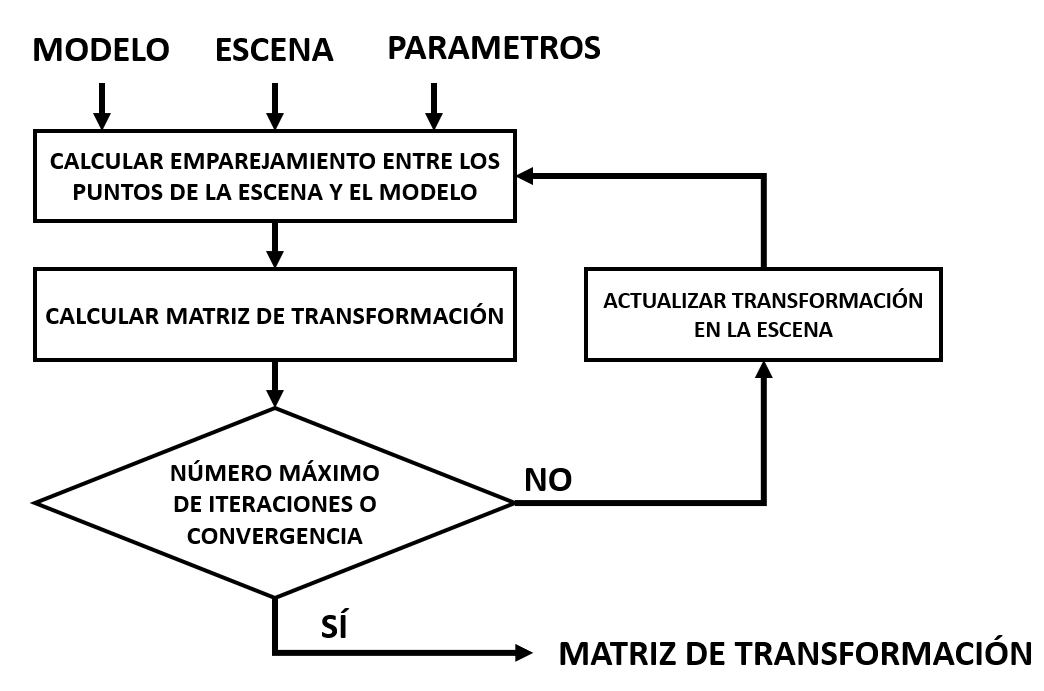
\includegraphics[height=8cm]{archivos/esquema-algoritmo-icp.png}
    \caption{Diagrama del algoritmo ICP.}
    \label{fig:esquema-algoritmo-icp}
\end{figure}

En la Figura \ref{fig:esquema-algoritmo-icp} podemos ver un esquema del funcionamiento del algoritmo \gls{icp}.
Este algoritmo recibe como parámetros de entrada la nube de puntos de la escena (fuente) y la nube de puntos del modelo (destino), además de los parámetros de configuración del algoritmo.
El algoritmo parte de la escena, que es la nube de puntos a alinear, y aplica diversas transformaciones con el objetivo de acercarse a la nube destino, el modelo.
El proceso se realiza de forma iterativa, partiendo en cada nueva iteración de la transformación anterior, hasta que finalmente la nube de puntos converge con el destino.
El resultado de aplicar el algoritmo \gls{icp} es la nube de puntos de la escena alineada, a la vez que una matriz de transformación final.
Si esta matriz de transformación la aplicamos sobre la nube de puntos de la escena original, obtendremos una nube de puntos de escena alineada con la nube de puntos del modelo.

Además, al método \gls{icp} original se pueden aplicar diferentes variaciones con la finalidad de mejorar su robustez.
Por ejemplo, se le puede añadir un parámetro para indicar el límite máximo de distancia para la correspondencia entre puntos, es decir, un valor que indique el radio de distancia desde cada punto en la nube de puntos de origen (escena) en el que la búsqueda de vecinos intentará encontrar un punto correspondiente en la nube de puntos de destino (modelo).
Este parámetro puede ser muy importante ya que limitar esta distancia ayuda en el rendimiento (cuanto menor sea el radio más rápido será) y puede evitar que el resultado no converja si la diferencia entre ambas nubes de puntos es muy grande.

\begin{figure}[h]
    \centering
    \begin{subfigure}[t]{0.33\textheight}
    	\centering
        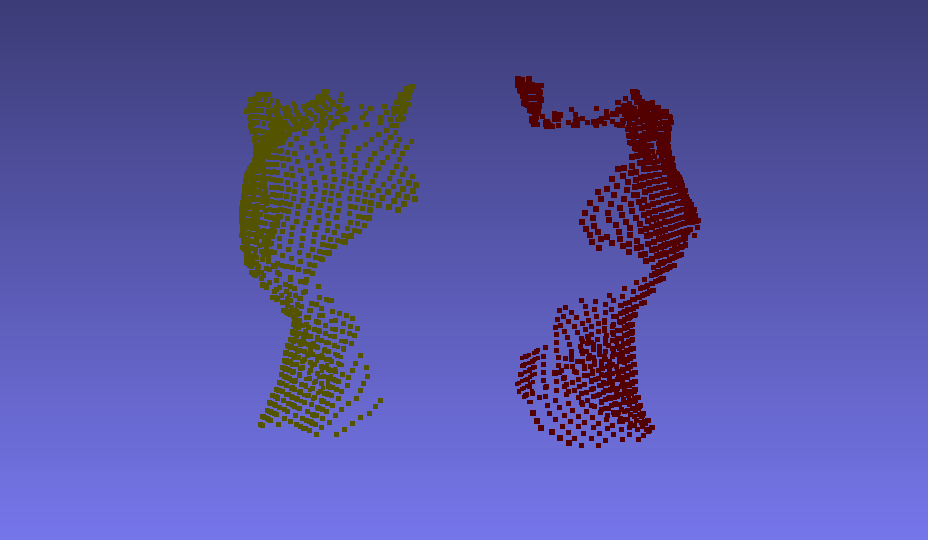
\includegraphics[height=4cm]{archivos/metodo-registro-explicacion-superpuesto-2-puntos.png}
        \caption{Modelo y escena superpuestos sin alinear.}
    \end{subfigure}
    \begin{subfigure}[t]{0.33\textheight}
    	\centering
        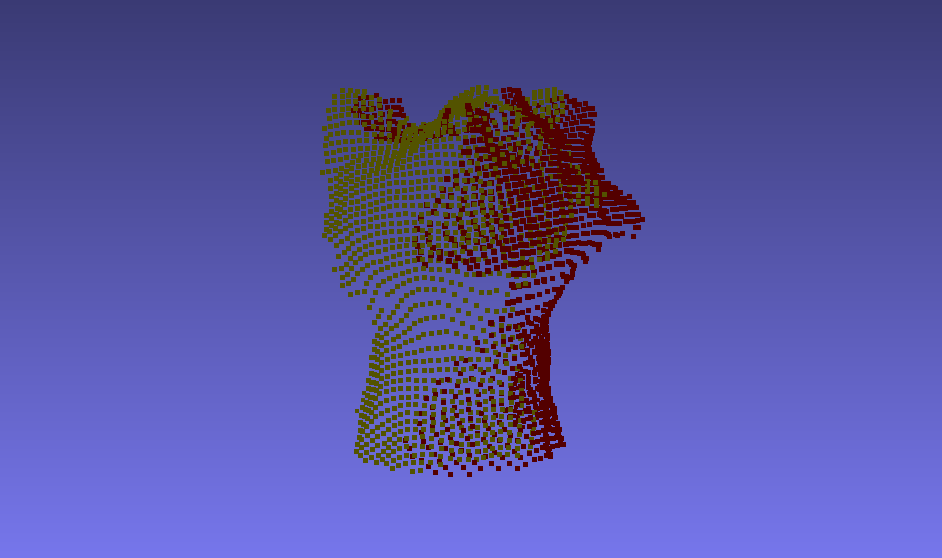
\includegraphics[height=4cm]{archivos/metodo-registro-explicacion-alineacion-puntos.png}
        \caption{Modelo y escena superpuestos alineados.}
    \end{subfigure}
    \caption{Ejemplo de captura de escena muy alejada al modelo.}
    \label{fig:modelo-escena-alejados-ejemplo}
\end{figure}

En la Figura \ref{fig:modelo-escena-alejados-ejemplo} podemos ver un caso donde gran parte de la nube de puntos de la escena no corresponden con el modelo, por tanto son pocos la cantidad de puntos que deberían coincidir entre ambas nubes.
En este caso, aplicar un umbral de distancia máxima entre correspondencias será muy útil para que el algoritmo \gls{icp} descarte los emparejamientos entre los puntos más lejanos.
También son importantes parámetros como el número de iteraciones máximas o el valor umbral para el error medio de emparejamiento que definirá la cantidad de iteraciones que el algoritmo \gls{icp} debe realizar para obtener la convergencia entre escena y modelo.

\subsection{Métodos de registro no rígidos, CPD}
\label{subsec:metodos-registro-no-rigido-cpd}

Mientras que una transformación rígida solo permite la traslación, rotación y escalado de la escena, la transformación no rígida permite tanto transformar afines, articulares y sesgos anisotrópicos.
Las aproximaciones simplistas de transformación no rígida verdadera, incluidos los modelos polinómicos y afines por partes, a menudo son inadecuadas para la alineación correcta y pueden producir correspondencias erróneas.
También suelen tener una alta complejidad computacional.
Además, debido al gran número de parámetros de transformación, los métodos de registro de nubes de puntos no rígidas tienden a ser sensibles al ruido y a los valores atípicos y es probable que converjan en mínimos locales.
Las degradaciones como el ruido, los valores atípicos y los puntos faltantes complican significativamente el problema.
Los valores atípicos son los puntos que se extraen incorrectamente de la imagen, estos valores atípicos no tienen correspondencias en el otro conjunto de puntos.

\gls{cpd} es un método de registro desarrollado originalmente por \cite{Myronenko2010}.
\gls{cpd} presenta un robusto algoritmo de registro de nubes de puntos probabilístico para transformaciones rígidas y no rígidas.
Mientras que \gls{icp} minimiza las distancias punto a punto, \gls{cpd} utiliza un \gls{mmg} para minimizar el error entre un punto y todos los demás puntos.
La alineación de dos nubes de puntos se considera como un problema de estimación de densidad de probabilidad, donde una nube de puntos representa los centroides del \gls{mmg} y el otro representa los puntos de datos.
Los centroides de \gls{mmg} se ajustan a los datos maximizando la probabilidad.
En el punto óptimo, las nubes de puntos se alinean y la correspondencia se obtiene usando las probabilidades posteriores de los componentes \gls{mmg}.
El núcleo del algoritmo es obligar a los centroides \gls{mmg} a moverse coherentemente como un grupo, lo que preserva la estructura topológica de los conjuntos de puntos.

El hecho de utilizar el \glsentrylong{mmg} entre punto y punto conlleva un rendimiento muy intensivo desde el punto de vista computacional.
Este algoritmo utiliza \gls{fgt}, una librería para acelerar las transformaciones gaussianas, también desarrollado por \cite{Myronenko2010}.
No obstante, tanto el algoritmo \gls{cpd} como los cálculos de errores subyacentes tardan mucho tiempo, a pesar de utilizar \gls{fgt}.

\section{Matriz de transformación 3D}

Como este \gls{tfg} utiliza tipos de datos \gls{3d}, los conceptos que se exponen serán enfocados a este tipo de datos.
La matriz de transformación \citep{wiki:transformation-matrix} es el resultado que obtenemos tras aplicar el método de registro.
Con la matriz de transformación, podemos transformar la nube de puntos de la escena y alinearla con la nube de puntos modelo.
La matriz de transformación se aplica directamente sobre una nube de puntos para transformarla.
Una nube de puntos es una matriz de $3\times\mathbf{N}$ donde $\mathbf{N}$ es la cantidad de puntos, para cada uno de los cuales tenemos el valor $\mathbf{X}$, $\mathbf{Y}$, $\mathbf{Z}$.\footnote{Una nube de puntos RGB, es decir, con color, será de $6\times\mathbf{N}$: los valores de posición $\mathbf{X}$, $\mathbf{Y}$, $\mathbf{Z}$; y los valores de color $\mathbf{R}$, $\mathbf{G}$, $\mathbf{B}$.
En estos casos, las matrices de transformación sólo se aplicarán a los valores $\mathbf{X}$, $\mathbf{Y}$, $\mathbf{Z}$.}
Al aplicar la matriz sobre la nube de puntos conseguimos transformarla, rotando y trasladando los puntos en su interior, con la finalidad, en este caso, de alinearlos con otra nube de puntos.

Una matriz de transformación está compuesta de una matriz de rotación y una matriz de traslación.

La matriz de rotación \citep{wiki:rotation-matrix} es una matriz $3\times3$ que contiene el valor por el que se necesita multiplicar cada uno de los puntos de una nube de puntos para ser rotada.
Una rotación básica consiste en una rotación que afecte solamente a uno de los ejes de coordenadas.
En la Ecuación \ref{eq:matrices-rotacion-basicas} podemos ver las tres matrices de rotación básicas para cada uno de los ejes, donde $\theta$ indica el ángulo con el que los ejes van a rotar.
Por ejemplo, si queremos rotar nuestra nube de puntos 15º grados en el eje $\mathbf{X}$, habría que aplicar la matriz de rotación $\mathbf{R}_{x}(15)$ a nuestra nube de puntos.
Tras multiplicar nuestra nube de puntos $3\times\mathbf{N}$ por esta matriz, obtendremos una nueva nube de puntos con nuevos valores que resultará en la misma nube de puntos rotada 15º en el eje $\mathbf{X}$, como se puede ver en el ejemplo de la Figura \ref{fig:modelo-rotado-15-eje-x}.

\begin{customequation}[h!]
    \begin{equation}
        \begin{aligned}
            \mathbf{R}_{x}(\theta)
            =
            \begin{vmatrix}
                1 & 0 & 0 \\
                0 & \cos\theta  & -\sin\theta \\
                0 & \sin\theta & \cos\theta
            \end{vmatrix}
            \\
            \\
            \mathbf{R}_{y}(\theta)
            =
            \begin{vmatrix}
                \cos\theta & 0 & \sin\theta \\
                0 & 1  & 0 \\
                -\sin\theta & 0 & \cos\theta
            \end{vmatrix}
            \\
            \\
            \mathbf{R}_{z}(\theta)
            =
            \begin{vmatrix}
                \cos\theta  & -\sin\theta & 0 \\
                \sin\theta & \cos\theta  & 0 \\
                0 & 0 & 1
            \end{vmatrix}
        \end{aligned}
    \end{equation}
    \caption{Matrices de rotación básicas.}
    \label{eq:matrices-rotacion-basicas}
\end{customequation}

\begin{figure}[h]
    \centering
    \begin{subfigure}[t]{0.33\textheight}
    	\centering
        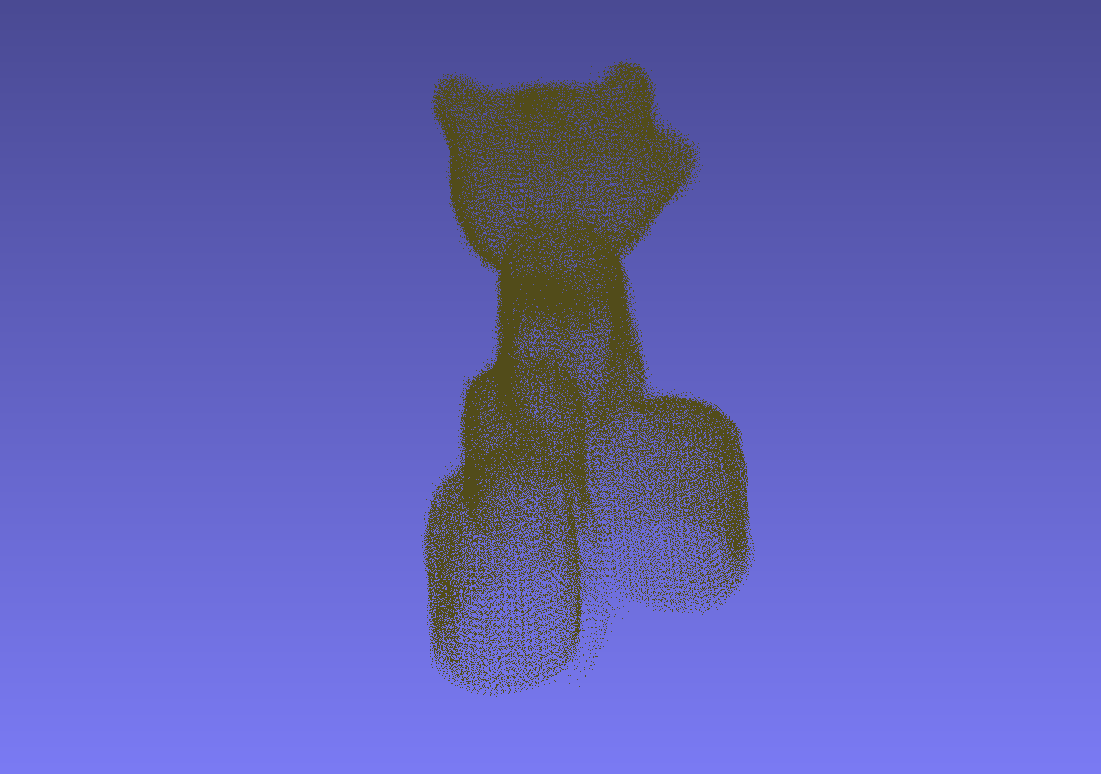
\includegraphics[height=4cm]{archivos/rotacion-15-original.png}
        \caption{Modelo 3D original.}
    \end{subfigure}
    \begin{subfigure}[t]{0.33\textheight}
    	\centering
        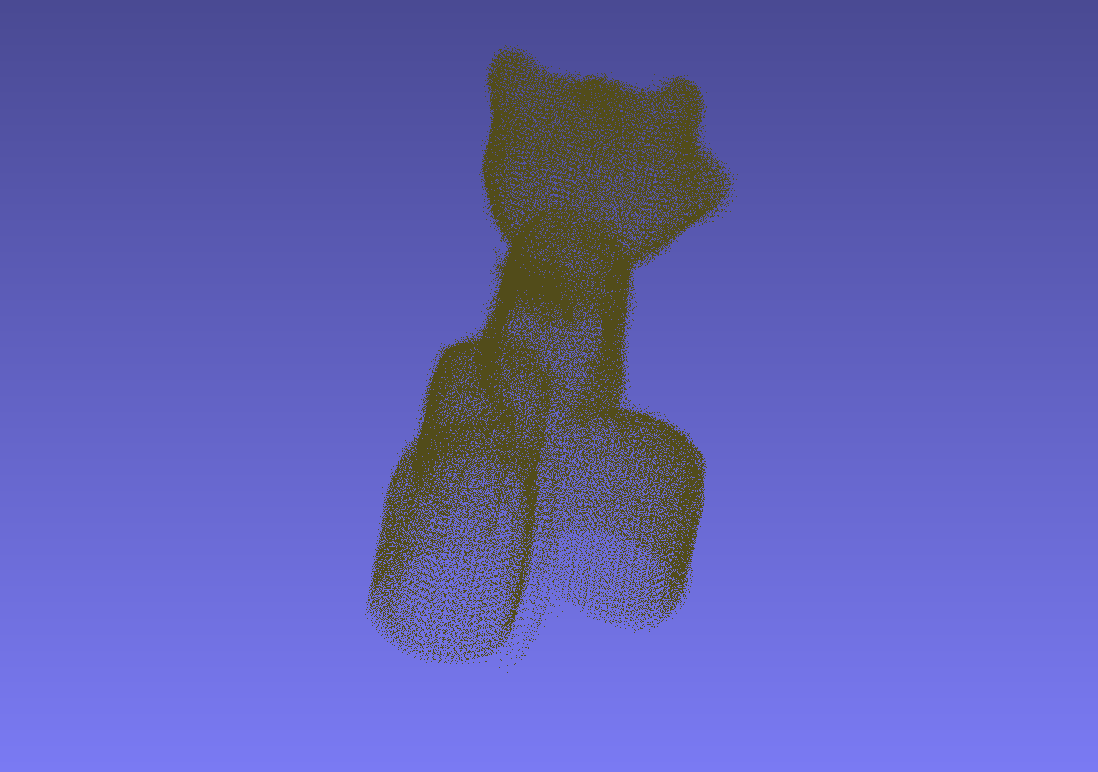
\includegraphics[height=4cm]{archivos/rotacion-15-rotado.png}
        \caption{Modelo 3D rotado 15º en el eje $\mathbf{X}$.}
    \end{subfigure}
    \caption{Rotación de 15º de un modelo 3D en el eje $\mathbf{X}$.}
    \label{fig:modelo-rotado-15-eje-x}
\end{figure}

La traslación \citep{wiki:translation-matrix} es una transformación geométrica que permite mover cada punto de la nube de puntos la misma distancia y en la misma dirección. Este movimiento puede ser representado en forma de vector o de matriz (Ecuación \ref{eq:vector-matriz-traslacion}).

\begin{customequation}[h!]
    \begin{equation}
        \mathbf{T}_{v}
        =
        \begin{vmatrix}
            v_{x} \\
            v_{y} \\
            v_{z}
        \end{vmatrix}
        \hspace{0.5cm}
        \mathbf{T}_{v}
        =
        \begin{vmatrix}
            1 & 0 & 0 & v_{x} \\
            0 & 1 & 0 & v_{y} \\
            0 & 0 & 1 & v_{z} \\
            0 & 0 & 0 & 1 \\
        \end{vmatrix}
    \end{equation}
    \caption{Vector y matriz de Traslación.}
    \label{eq:vector-matriz-traslacion}
\end{customequation}

La traslación es una transformación afín sin puntos fijos, sin embargo, la multiplicación en las matrices siempre tienen su origen como punto fijo.
Para solucionar este inconveniente, al vector de 3 dimensiones $\mathbf {v}=(v_{x},v_{y},v_{z})$ se le añade una dimensión más $\mathbf {v}=(v_{x},v_{y},v_{z},1)$, de esta forma conseguimos trabajar utilizando coordenadas homogéneas para representar la traslación en un espacio vectorial con multiplicación de matrices.
Como podemos ver en la Ecuación \ref{eq:matriz-traslacion-aplicada}, se está multiplicando una matriz de traslación por uno de los puntos de una nube de puntos.
El resultado de esta multiplicación consiste en ese mismo punto sumándole el movimiento de la matriz de traslación.

\begin{customequation}[h!]
    \begin{equation}
        \mathbf{T}_{v}
        \mathbf{p}
        =
        \begin{vmatrix}
            1 & 0 & 0 & v_{x} \\
            0 & 1 & 0 & v_{y} \\
            0 & 0 & 1 & v_{z} \\
            0 & 0 & 0 & 1 \\
        \end{vmatrix}
        \begin{vmatrix}
            p_{x} \\
            p_{y} \\
            p_{z} \\
            1 \\
        \end{vmatrix}
        =
        \begin{vmatrix}
            p_{x} + v_{x} \\
            p_{y} + v_{y} \\
            p_{z} + v_{z} \\
            1 \\
        \end{vmatrix}
        = p + v
    \end{equation}
    \caption{Matriz de Traslación aplicada a un punto.}
    \label{eq:matriz-traslacion-aplicada}
\end{customequation}

Por tanto, una matriz de transformación no es más que la combinación de un matriz de rotación y una matriz de transformación, dando lugar a una matriz $4x4$ que contiene la información de ambas matrices (Ecuación \ref{eq:matriz-transformacion}). Para más detalles, se recomienda leer "Multiple view geometry in computer vision" de \cite{hartley2003multiple}.

\begin{customequation}[h!]
    \begin{equation}
        \mathbf{T} =
        \begin{vmatrix}
            \mathbf{r}_{0,0} & \mathbf{r}_{0,1} & \mathbf{r}_{0,2} & \mathbf{v}_{x} \\
            \mathbf{r}_{1,0} & \mathbf{r}_{1,1} & \mathbf{r}_{1,2} & \mathbf{v}_{y} \\
            \mathbf{r}_{2,0} & \mathbf{r}_{2,1} & \mathbf{r}_{2,2} & \mathbf{v}_{z} \\
            0 & 0 & 0 & 1
        \end{vmatrix}
    \end{equation}
    \caption{Matriz de Transformación.}
    \label{eq:matriz-transformacion}
\end{customequation}

La matriz de transformación contiene información importante no solo para la alineación de una escena con el modelo, sino para la reconstrucción de todo el cuerpo \gls{3d} a partir de varias escenas distintas, ya que será necesario tener en cuenta cada una de las transformaciones aplicadas para usarlas como transformación inicial en una nueva escena a alinear.

Por ejemplo, si hemos realizado 3 capturas desde distintos ángulos (Figuras \ref{fig:ejemplo-acumulacion-transformacion-captura-1}, \ref{fig:ejemplo-acumulacion-transformacion-captura-2}, \ref{fig:ejemplo-acumulacion-transformacion-captura-3}), tomaremos la captura 1 como modelo, y las capturas 2 y 3 como escenas que hay que alinear con el modelo.
Tras conseguir la matriz de transformación que alinea la captura 2 (escena) con la captura 1 (modelo), nuestra captura 2 transformada pasará a convertirse también en el modelo, pues estará alineada con la captura 1 (Figura \ref{fig:ejemplo-acumulacion-transformacion-captura-2-alineada}).
Para alinear la captura 3 (nueva escena) con las capturas 1 y 2 (actual modelo) se le aplicará a la captura 3 como transformación inicial el resultado de alinear la captura 2 con la 1 (Figura \ref{fig:ejemplo-acumulacion-transformacion-captura-3-transformacion-inicial}), de esta forma, la captura 3 se acercará un poco más al modelo (capturas 1 y 2).
Seguidamente volvemos a aplicar el método de registro para obtener la captura 3 alineada (Figura \ref{fig:ejemplo-acumulacion-transformacion-captura-3-alineada}).
% En una futura captura 4 a alinear con las capturas 1, 2 y 3 (modelo), se le aplicará tanto la matriz de transformación del registro de la 2 a la 1, como la transformación del registro de la 3 a la 2 y 1.

\begin{figure}[h]
    \centering
    \begin{subfigure}[t]{0.2\textheight}
    	\centering
        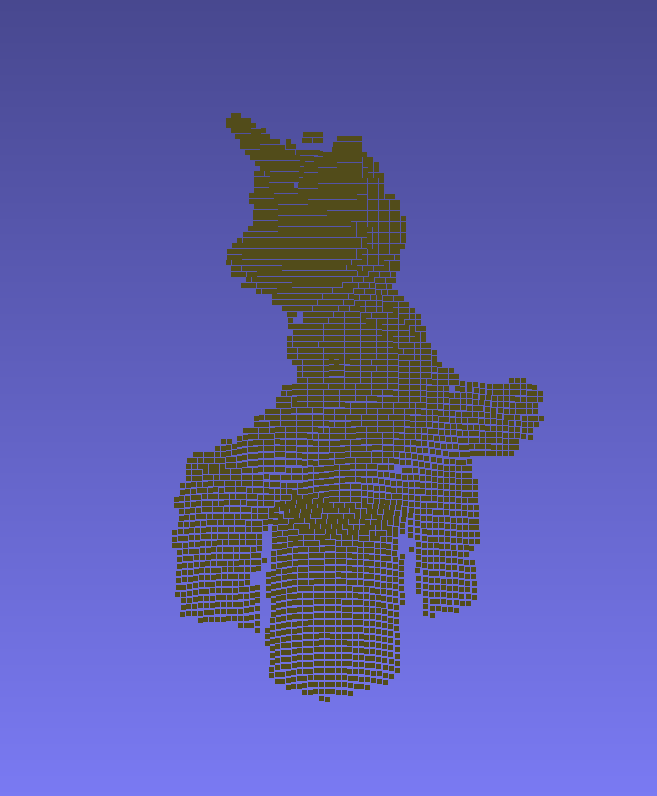
\includegraphics[height=4cm]{archivos/ejemplo-acumulacion-transformacion-captura-1.png}
        % Captura 1, 2 y 3 pero la 1 superpuesta por encima
        \caption{Captura 1.}
        \label{fig:ejemplo-acumulacion-transformacion-captura-1}
    \end{subfigure}
    \begin{subfigure}[t]{0.2\textheight}
    	\centering
        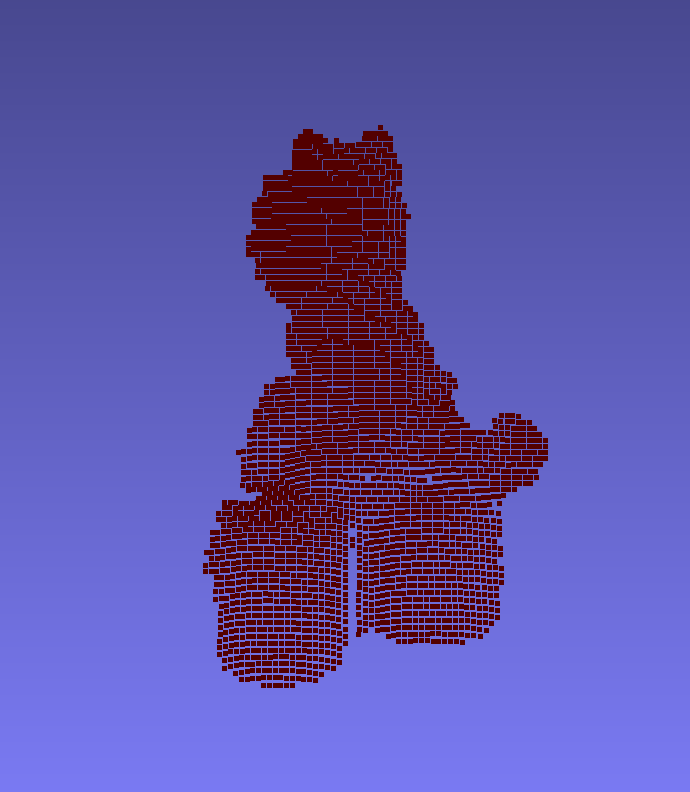
\includegraphics[height=4cm]{archivos/ejemplo-acumulacion-transformacion-captura-2.png}
        % Captura 1, 2 y 3 pero la 2 superpuesta por encima
        \caption{Captura 2.}
        \label{fig:ejemplo-acumulacion-transformacion-captura-2}
    \end{subfigure}
    \begin{subfigure}[t]{0.2\textheight}
    	\centering
        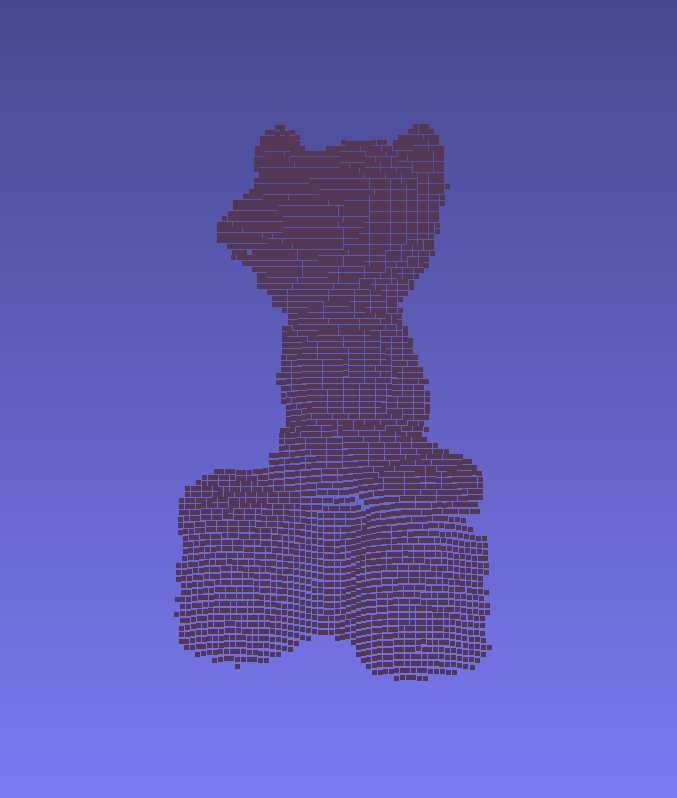
\includegraphics[height=4cm]{archivos/ejemplo-acumulacion-transformacion-captura-3.png}
        % Captura 1, 2 y 3 pero la 3 superpuesta por encima
        \caption{Captura 3.}
        \label{fig:ejemplo-acumulacion-transformacion-captura-3}
    \end{subfigure}
    \begin{subfigure}[t]{0.2\textheight}
    	\centering
        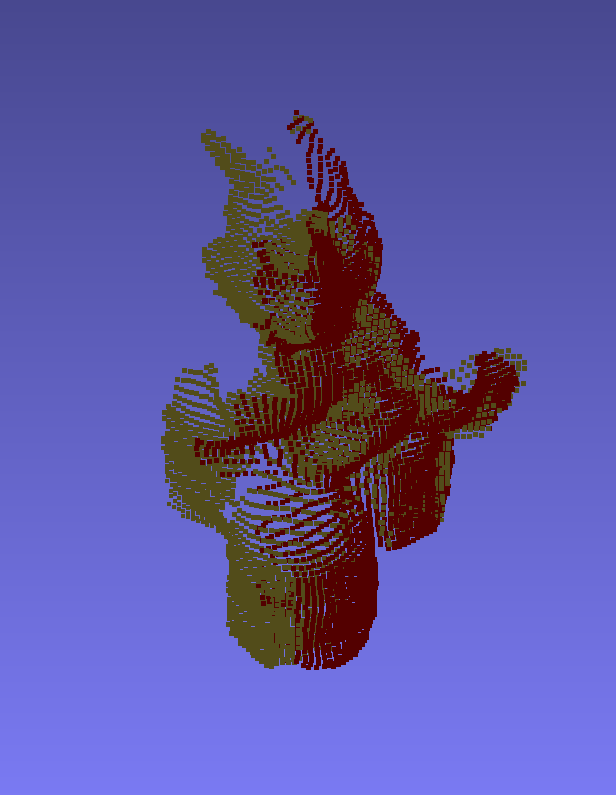
\includegraphics[height=4cm]{archivos/ejemplo-acumulacion-transformacion-captura-2-alineada.png}
        % Captura 1 y 2 alineadas y la 3, pero la 1 y 2 superpuestas por encima
        \caption{Captura 2 (escena) alineada con la captura 1 (modelo).}
        \label{fig:ejemplo-acumulacion-transformacion-captura-2-alineada}
    \end{subfigure}
    \begin{subfigure}[t]{0.2\textheight}
    	\centering
        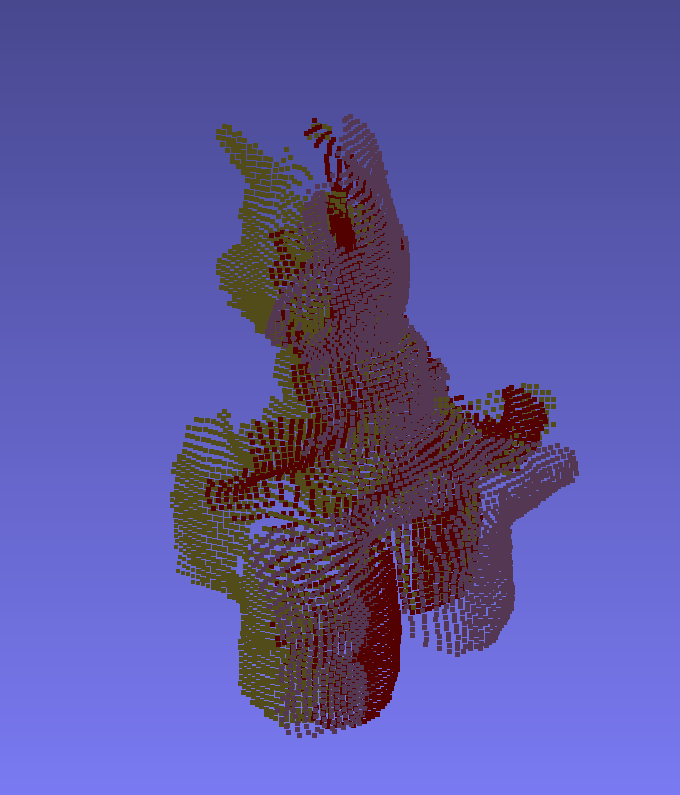
\includegraphics[height=4cm]{archivos/ejemplo-acumulacion-transformacion-captura-3-transformacion-inicial.png}
        % Captura 1 y 2 alineadas y la 3, 3 superpuesta por encima
        \caption{Captura 3 con transformación inicial.}
        \label{fig:ejemplo-acumulacion-transformacion-captura-3-transformacion-inicial}
    \end{subfigure}
    \begin{subfigure}[t]{0.2\textheight}
    	\centering
        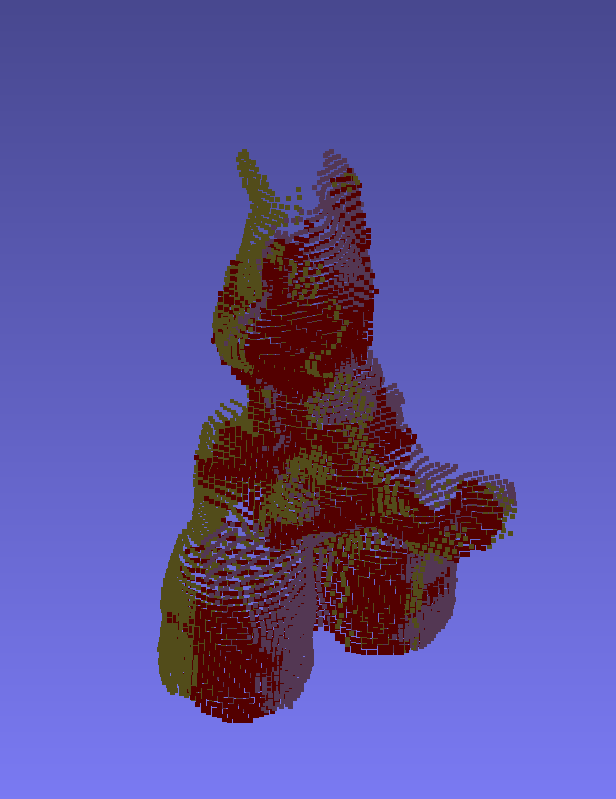
\includegraphics[height=4cm]{archivos/ejemplo-acumulacion-transformacion-captura-3-alineada.png}
        % Captura 1, 2 y 3 alineadas
        \caption{Captura 3 (escena) alineada con 1 y 2 (modelo).}
        \label{fig:ejemplo-acumulacion-transformacion-captura-3-alineada}
    \end{subfigure}
    \caption{Ejemplo de matriz de transformación inicial.}
    \label{fig:ejemplo-acumulacion-transformacion}
\end{figure}

\section{Filtros para el pre-procesamiento y post-procesamiento de los datos}

Tras la fase de adquisición, donde obtenemos una nube de puntos que identificamos como modelo y el resto de nube de puntos que identificamos como escenas, es buena idea hacer uso de filtros sobre las nubes de puntos en una fase de pre-procesamiento antes de ser enviadas al método de registro donde serán finalmente procesadas.
Esto puede ayudar al método de registro para que funcione mejor encontrando las correspondencias entre las nubes de puntos.

Además, tras ser procesadas por el método de registro, también se puede volver a aplicar otros filtros en una fase de post-procesamiento. Este filtro de post-procesamiento puede ayudar a obtener un resultado de mayor calidad para la fase final de análisis.

En la Figura \ref{fig:diagrama-filtros-pre-post-procesamiento} podemos ver un esquema que muestra en qué momento se aplicarán los filtros de pre-procesamiento y post-procesamiento.

\begin{figure}[h]
    \centering
    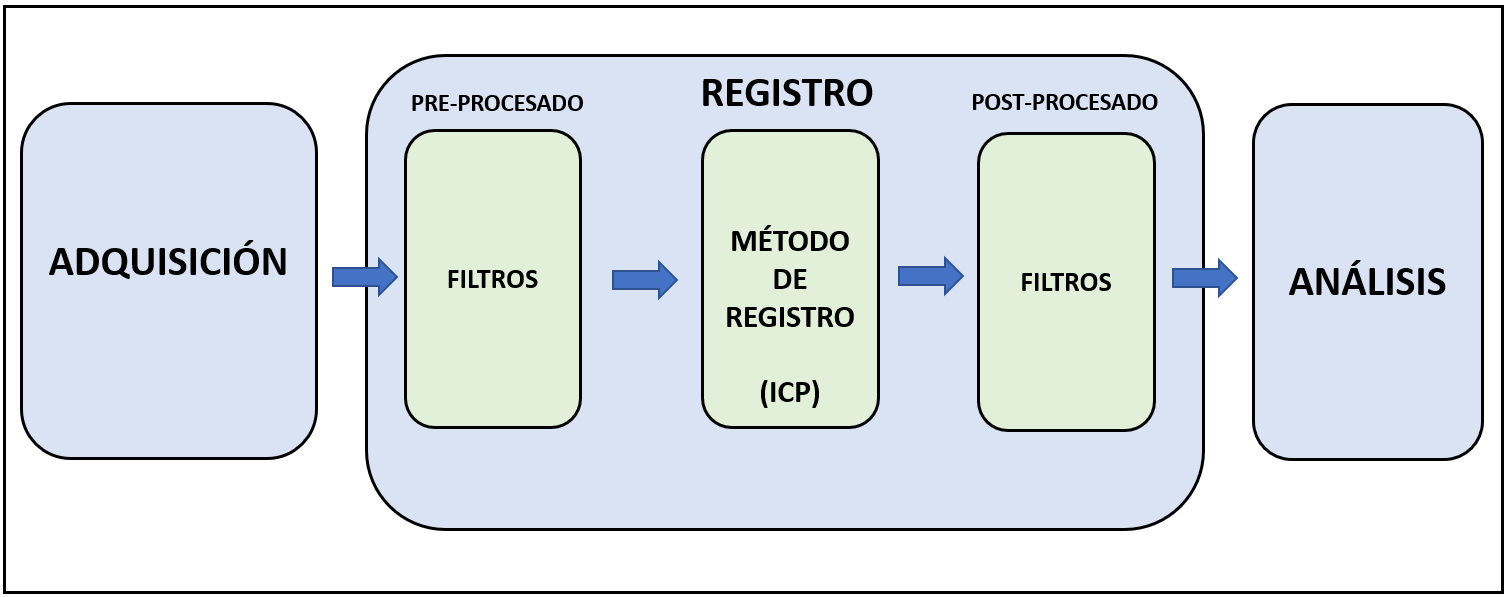
\includegraphics[height=6cm]{archivos/diagrama-filtros-pre-post-procesamiento.png}
    \caption{Filtros de pre-procesamiento y post-procesamiento en un esquema general de un sistema 3D.}
    \label{fig:diagrama-filtros-pre-post-procesamiento}
\end{figure}

A continuación, se detallarán una serie de filtros que se aplicarán en fase de pre-procesado que harán que el método de registro funcione mejor.

\begin{description}

    \item[Filtro de diezmado (Decimation Filter):]
    
    el filtro de diezmado ayuda a eliminar el exceso de ancho de banda y reduce la frecuencia de muestreo de la señal a una frecuencia de muestreo más baja que difiere de la frecuencia original en un valor entero.
    También ayuda a reducir los recursos computacionales necesarios para procesar y almacenar la señal \citep{engineerAmbitiosly}.

    La razón para aplicar este filtro normalmente consiste en reducir la frecuencia de muestreo en la salida de un sistema para que un sistema que opera a una frecuencia de muestreo más baja pueda ingresar la señal.
    Pero una motivación mucho mayor para diezmar, y motivo por el cual es interesante para este proyecto, es reducir el costo de procesamiento al tratar con los datos tras ser aplicado el filtro. Gracias a este filtro obtenemos una nube de puntos con menor cantidad de puntos, lo cual permitirá al método de registro trabajar más rápido.

    Este filtro es muy parecido al downsampling, sin perder demasiada calidad en la nube de puntos. El uso de este filtro está recomendado en la documentación de Intel, y proporcionan un método en la librería de RealSense para aplicarlo a la hora de tomar la captura.
    
    % \item[Reducción de muestreo (Downsampling):]
    
    % el filtro consiste en reducir la cantidad total de puntos en la muestra, obteniendo solo un conjunto de datos de nube de puntos, utilizando un enfoque de cuadrícula voxelizada.

    % La implementación de este filtro por \gls{pcl} consiste en crear una cuadrícula de vóxeles\footnote{Un vóxel es la unidad cúbica que compone un objeto tridimensional. Constituye la unidad mínima procesable de una matriz tridimensional y es, por tanto, el equivalente del píxel en un objeto 2D.} 3D sobre los datos de la nube de puntos de entrada.
    % Luego, en cada vóxel, se aproximarán todos los puntos presentes con su centroide.
    % Este enfoque es un poco más lento que aproximarlos con el centro del vóxel, pero representa la superficie subyacente con mayor precisión.

    % Por tanto, con la aplicación de este filtro obtendremos una nube de puntos más reducida pero con la suficiente calidad para que el método de registro funcione adecuadamente.    

    \item[PassThrough Filter:]
    
    este filtro consiste en definir unos valores para cada dimensión donde la nube de puntos será recortada.
    Es decir, se especifica un rango para las dimensiones $\mathbf{X}$, $\mathbf{Y}$, $\mathbf{Z}$, y todo lo que esté fuera de dicho rango será recortado de la nube de puntos.

    Con este filtro conseguimos por una parte, reducir la cantidad de puntos finales, con lo que conseguimos una nube de puntos más liviana y, como se ha comentado en los filtros anteriores, esto hará que el método de registro funcione más rápido.
    Pero lo más importante es que podemos eliminar la parte de la nube de puntos que no nos interesa y que, además, podría entorpecer en el funcionamiento del método de registro.
    Por ejemplo, si lo que estamos capturando con el sensor es una persona dando vueltas en el mismo sitio, todos los objetos, paredes y entorno que le rodea no es información relevante para el registro.
    De hecho, puede provocar un peor funcionamiento si se dejara, pues son puntos fijos que no cambian entre captura y captura.

    \item[Statistical Outlier Removal Filter:]
    
    este filtro es muy interesante porque nos permite eliminar valores atípicos en la nube de puntos, que probablemente serán mediciones ruidosas que ha capturado el sensor.
    Los errores de medición en la fase de adquisición conducen a valores atípicos dispersos que corrompen los resultados del registro.

    La eliminación estadística de valores atípicos funciona realizando un análisis estadístico de la vecindad de cada punto y recortando aquellos que no cumplen con un determinado criterio.
    La eliminación de valores atípicos dispersos se basa en el cálculo de la distribución de puntos a distancias vecinas en el conjunto de datos de entrada.
    Para cada punto, se calcula la distancia media desde él a todos sus vecinos.
    Todos los puntos cuyas distancias medias están fuera de un intervalo definido por la media y la desviación estándar de las distancias globales pueden considerarse valores atípicos y recortarse del conjunto de datos.

    Por tanto el uso de este filtro nos permite obtener una nube de puntos más limpia eliminando los puntos lejanos, puntos atípicos y que no corresponden con el objeto o cuerpo capturado.

    \item[Filtro de mediana (Median Filter):]
    
    El filtro de la mediana es uno de los filtros de procesamiento de imágenes más simples y más extendidos, se sabe que funciona bien con ruido de disparo o ruido de impulso.\footnote{El ruido de disparo o de impulso son píxeles individuales que tienen valores extremos.}
    Es simple de implementar y eficiente, ya que requiere una sola pasada sobre la imagen. Consiste en una ventana móvil de tamaño fijo que reemplaza el píxel del centro por la mediana dentro de la ventana.

\end{description}

Los filtros de eliminación estadística de valores atípico (Statistical Outlier Removal) y de mediana también son filtros muy interesantes para aplicar en la fase de post-procesado, ya que además de permitir un mejor funcionamiento durante el método de registro, mejora la calidad de la nube de puntos resultante.

\section{Aceleración por GPU, CUDA}

Los métodos de registro \gls{2d} y \gls{3d} suelen proporcionar buenos resultados, sin embargo presentan restricciones temporales debido a su naturaleza secuencial y a la gran cantidad de cálculos que deben realizar.
Es por ello que se buscan métodos para acelerar dichos algoritmos que minimicen todo lo posible las restricciones temporales.
La forma tradicional de aceleración aplicada a estos métodos es la computación paralela.

El paradigma \gls{gpgpu} \citep{Luebke2006} es un concepto dentro de la informática que trata de estudiar y aprovechar las capacidades de cómputo de una \gls{gpu}.
Inicialmente los dispositivos \gls{gpu} se utilizaban únicamente para el procesamiento de los gráficos de un ordenador cuyos datos a tratar estaban enfocados a ser convertidos a formato gráfico.
En la actualidad combinan su gran potencia de cálculo para albergar cálculos paralelos de propósito general en los que se trabaja con grandes cantidades de datos que no tienen por qué ser convertidos a formato gráfico.

Existen dos tecnologías principales para la programación en dispositivos \gls{gpu}: \glsentryfull{cuda} y \gls{opencl}.
En un principio la programación para aprovechar las características de este tipo de dispositivos debía hacerse mediante código ensamblador.
Sin embargo, hoy día existen alternativas con lenguajes de alto nivel que facilitan el desarrollo de las aplicaciones.
\gls{cuda} \citep{Luebke2008} es una plataforma de computación en paralelo que incluye un compilador y un conjunto de herramientas de desarrollo creadas por Nvidia que permite utilizar una variación del lenguaje de programación C (CUDA C) para codificar algoritmos en \gls{gpu}s de Nvidia.
\gls{opencl} \citep{Stone2010} por su parte consta de una interfaz de programación de aplicaciones y de un lenguaje de programación que permiten crear aplicaciones con paralelismo a nivel de datos y de tareas que pueden ejecutarse en \gls{gpu}.
Se trata de una alternativa a \gls{cuda} de código libre y abierta.

Los dispositivos \gls{gpu}s consiguen mejor rendimiento que las \gls{cpu}s procesando datos en coma flotante debido a su arquitectura.
Como podemos ver en la Figura \ref{fig:comparacion-cpu-gpu} \citep{Stopper2017}, un dispositivo \gls{gpu} está diseñado para el cálculo intensivo altamente paralelo, por lo que tiene más transistores destinados al procesamiento de datos que al flujo de control o a la caché de datos.
Las \gls{gpu}s son dispositivos especialmente adecuados para resolver problemas que puedan expresarse como cálculos con datos realizados
simultáneamente, ejecutando el mismo programa sobre muchos datos en paralelo.
Los cálculos que se realizan conllevan una alta intensidad aritmética, es decir, un elevado ratio de operaciones aritméticas por operación de memoria, lo que hace innecesaria la utilización de grandes cantidades de caché de datos.

\begin{figure}[h]
    \centering
    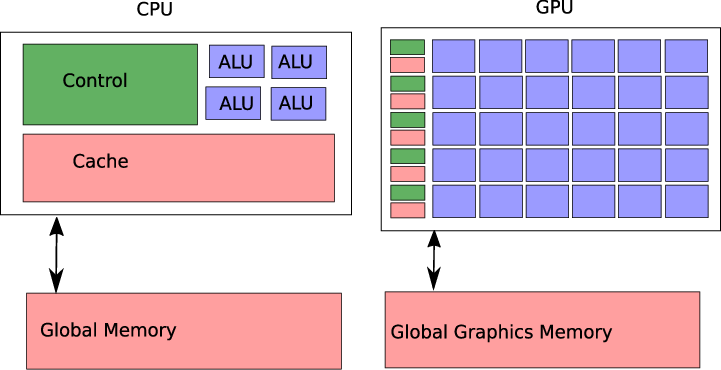
\includegraphics[width=0.7\linewidth]{archivos/comparativa-cpu-gpu.png}
    \caption{Comparación de arquitecturas CPU y GPU. Figura extraída de \cite{Stopper2017}.}
    \label{fig:comparacion-cpu-gpu}
\end{figure}

\gls{cuda} es una arquitectura con modelo \gls{simt}, es decir, una instrucción, múltiples hilos.
Estos hilos se ejecutan simultáneamente, trabajando sobre grandes cantidades de datos en paralelo.
En la Figura \ref{fig:arquitectura-gpu-cuda} \citep{peter2009nvidia} podemos ver la estructura de los dispositivos \gls{gpu} compatibles con la arquitectura \gls{cuda}, los cuales están formados por un conjunto de multiprocesadores.
Estos multiprocesadores reciben el nombre de \gls{sm} y permiten trabajar con múltiples hilos en paralelo.
Sin embargo, el número de multiprocesadores varía dependiendo de la arquitectura de la \gls{gpu}. Cada \gls{sm} se compone de una serie de \gls{sp} que comparten la lógica de control y la memoria caché.
Cada uno de estos \gls{sp} puede lanzar una gran cantidad de hilos en paralelo.

\begin{figure}[h]
    \centering
    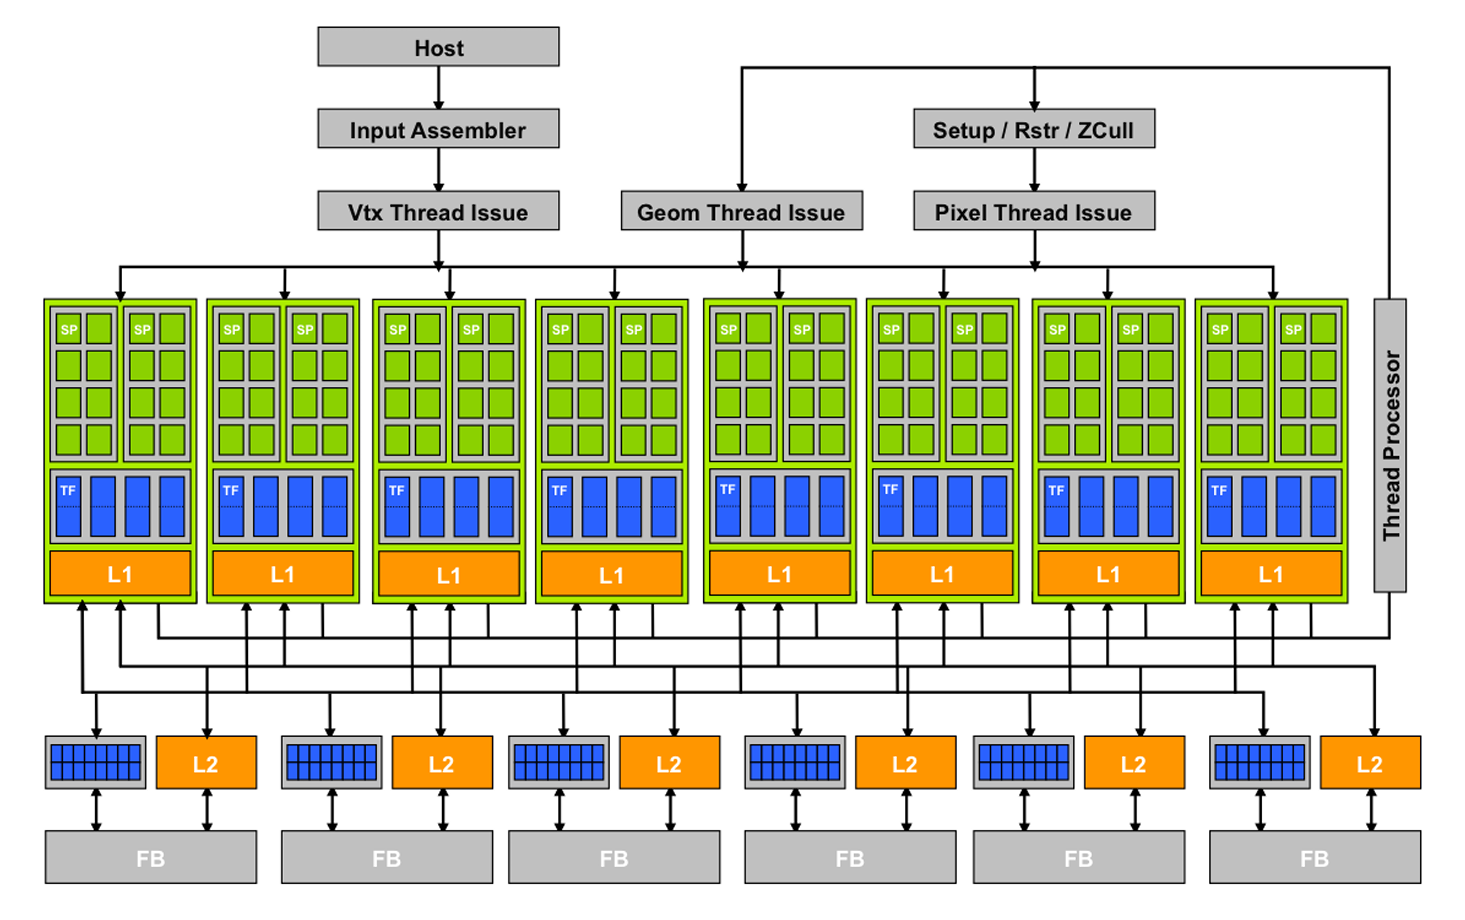
\includegraphics[width=\linewidth]{archivos/diagrama-arquitectura-cuda.png}
    \caption{Arquitectura GPU con tecnología CUDA. Figura extraída de \cite{peter2009nvidia}.}
    \label{fig:arquitectura-gpu-cuda}
\end{figure}

Una vez definida la importancia de los dispositivos \gls{gpu} para la resolución de problemas de cálculo intensivo a los que se aplican computación paralela, para utilizar estos dispositivos con el objetivo de acelerar un determinado algoritmo será necesario realizar un rediseño del algoritmo que se adapte a la arquitectura de la \gls{gpu}.
Para paralelizar un algoritmo de forma eficiente será necesario identificar claramente unidades de trabajo independientes capaces de trabajar con subconjuntos de datos.
Este es un aspecto crítico a la hora de rediseñar un algoritmo para que funcione concurrentemente.

El algoritmo \gls{icp} requiere mucho tiempo de proceso en la \gls{cpu} debido a la gran cantidad de operaciones que deben realizar en cada una de sus etapas, concretamente la encargada de calcular los emparejamientos entre las nubes de puntos escena y modelo.
En esta etapa es donde se encuentra el principal cuello de botella del algoritmo \gls{icp}, ya que el algoritmo debe encontrar para cada punto de la escena el punto del modelo más cercano.
Esta etapa del algoritmo realizada en la \gls{cpu} de forma secuencial emplea una gran cantidad de tiempo.
Muchas de estas operaciones se pueden realizar en paralelo ya que son independientes y trabajan sobre el mismo conjunto de datos, lo cual hace que el algoritmo cumpla con los requisitos básicos para poder ser implementado de forma paralela, orientado a su ejecución en una \gls{gpu}, de esta manera se puede reducir notablemente el tiempo de procesamiento que emplea el algoritmo.

Existen varias implementaciones desarrolladas en \gls{gpu} del algoritmo \gls{icp} \citep{Langis} \citep{barsukov2013development}.
Incluso Nvidia ha creado oficialmente un repositorio con implementaciones sobre la librería \gls{pcl}, incluyendo una implementación sobre el algoritmo \gls{icp} \citep{LeiFan}.

\chapter{Intel RealSense Depth Camera D435}
\label{cap:realsense-d435}

Este \gls{tfg} se enmarca en un proyecto que utiliza la cámara \gls{rgbd} Intel RealSense Depth Camera D435, por lo que aquí se explica el funcionamiento de esta.

Intel RealSense Depth Camera D435 es un sensor \gls{rgbd} de propósito general. 
Este sensor \gls{3d} tiene una profundidad mínima de 0,2 metros y escanea entornos de hasta 10 metros de ancho con una profundidad de resolución de hasta 1280x720 a 90 fotogramas por segundo (fps).
El sistema utiliza un procesador Intel D4vision de 28 nanómetros para procesar datos de profundidad complejos en tiempo real y un procesador de imágenes en color Realtek.
El proyector láser \gls{ir} mide solo 2,7x1,8 milímetros, utiliza tecnología \gls{vcsel} y puede grabar 60 fps.
El dispositivo RealSense D435 tiene tres sensores para capturar la imagen: un sensor CMOS 1080p RGB para capturar imágenes con color y dos sensores de 1 megapíxel a los lados izquierdo y derecho del sensor \gls{ir} \gls{vcsel}.
Estos dos últimos sensores son utilizados para obtener las imágenes en profundidad mediante una tecnología estéreo activa.
El sensor es capaz de proporcionar imágenes de alta definición gracias al procesador de visión, el proyector \gls{vcsel} y el sensor de imagen.
En la Figura \ref{fig:d435-sensors2} podemos ver los sensores descritos en el Intel RealSense D435.

\begin{figure}[h]
    \centering
    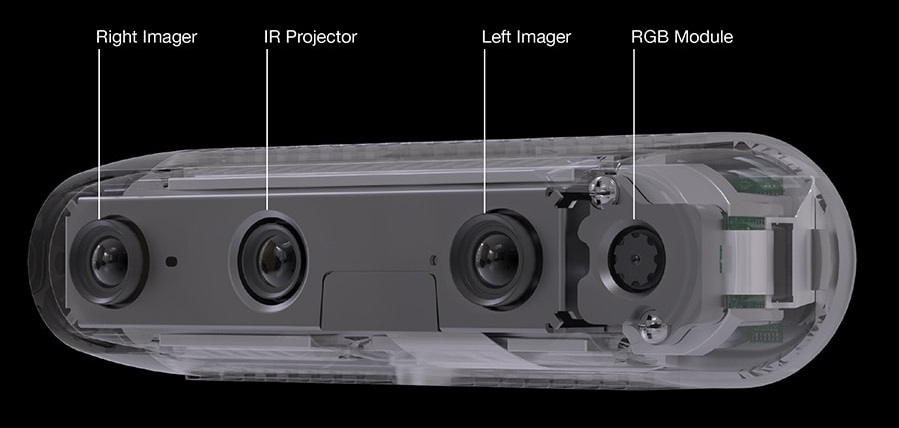
\includegraphics[width=0.7\textwidth]{archivos/d435_sensors.jpg}
    \caption{Sensores Intel RealSense D435.}
    \label{fig:d435-sensors2}
\end{figure}

La tecnología estéreo activa, o ``Active Stereo'' en inglés, funciona por triangulación.
El sensor puede ver el mismo punto desde dos ubicaciones diferentes, desde el sensor de 1 megapíxel ubicado a la izquierda del sensor \gls{vcsel} y desde el sensor de 1 megapíxel ubicado a la derecha.
Con esta información puede usar la trigonometría para medir la distancia real que hay desde el sensor hasta el punto.
Tras identificar un punto común en ambas imágenes, usa el ángulo conocido de cada sensor para cada imagen y la distancia entre ambos sensores para calcular la distancia.
Para ello, el sensor tiene un calibrado interno sobre el ángulo y distancia de ambos sensores.
Cuanto más larga es la distancia entre los sensores de imagen, más precisa es la medición.
En la Figura \ref{fig:ejemplo-sensor-estereo-activo} podemos ver un ejemplo donde para un punto común, conociendo el ángulo 'a' y 'b', y la distancia entre los sensores, se puede calcular la distancia al punto común.

\begin{figure}[h]
    \centering
    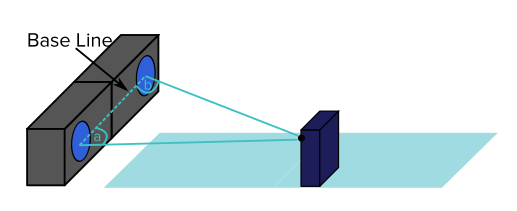
\includegraphics[width=0.7\textwidth]{archivos/ejemplo-sensor-estereo-activo.png}
    \caption{Ejemplo de identificación de un punto común con tecnología estéreo activa. Figura extraída de \cite{rafaelWhyte}.}
    \label{fig:ejemplo-sensor-estereo-activo}
\end{figure}

Con la tecnología estéreo activa, es importante hacer coincidir las mismas características en ambas imágenes.
Una forma de mejorar esto es proyectar patrones de puntos, cada sensor de profundidad puede identificar cada punto único.
De esta forma, la proyección de puntos facilita la coincidencia de características y permite medir objetos sin características, como paredes blancas.

El D435 utiliza la combinación de estéreo activo y pasivo, por lo que puede medir objetos más cercanos sin rasgos distintivos y objetos más lejanos.

\chapter{Propuesta de solución}
\label{cap:propuesta-de-solucion}

El objetivo del \gls{tfg} consiste en desarrollar un sistema que reconstruya un cuerpo humano completo, utilizando como sensor para la adquisición de los datos el Intel RealSense D435 y el sistema embebido Jetson Nano como computador que procesará los datos en la fase de registro.
Por ello, en este capítulo detallaremos cuales han sido los pasos a seguir para conseguir un sistema que funcione y sea capaz de llevar a cabo esta reconstrucción.

En la Figura \ref{fig:diagrama-propuesta-solucion} podemos ver un diagrama de la implementación de los módulos del sistema, desde la fase de adquisición, pasando por la fase de registro, hasta la fase de análisis con los resultados finales.

\begin{figure}[h]
    \centering
    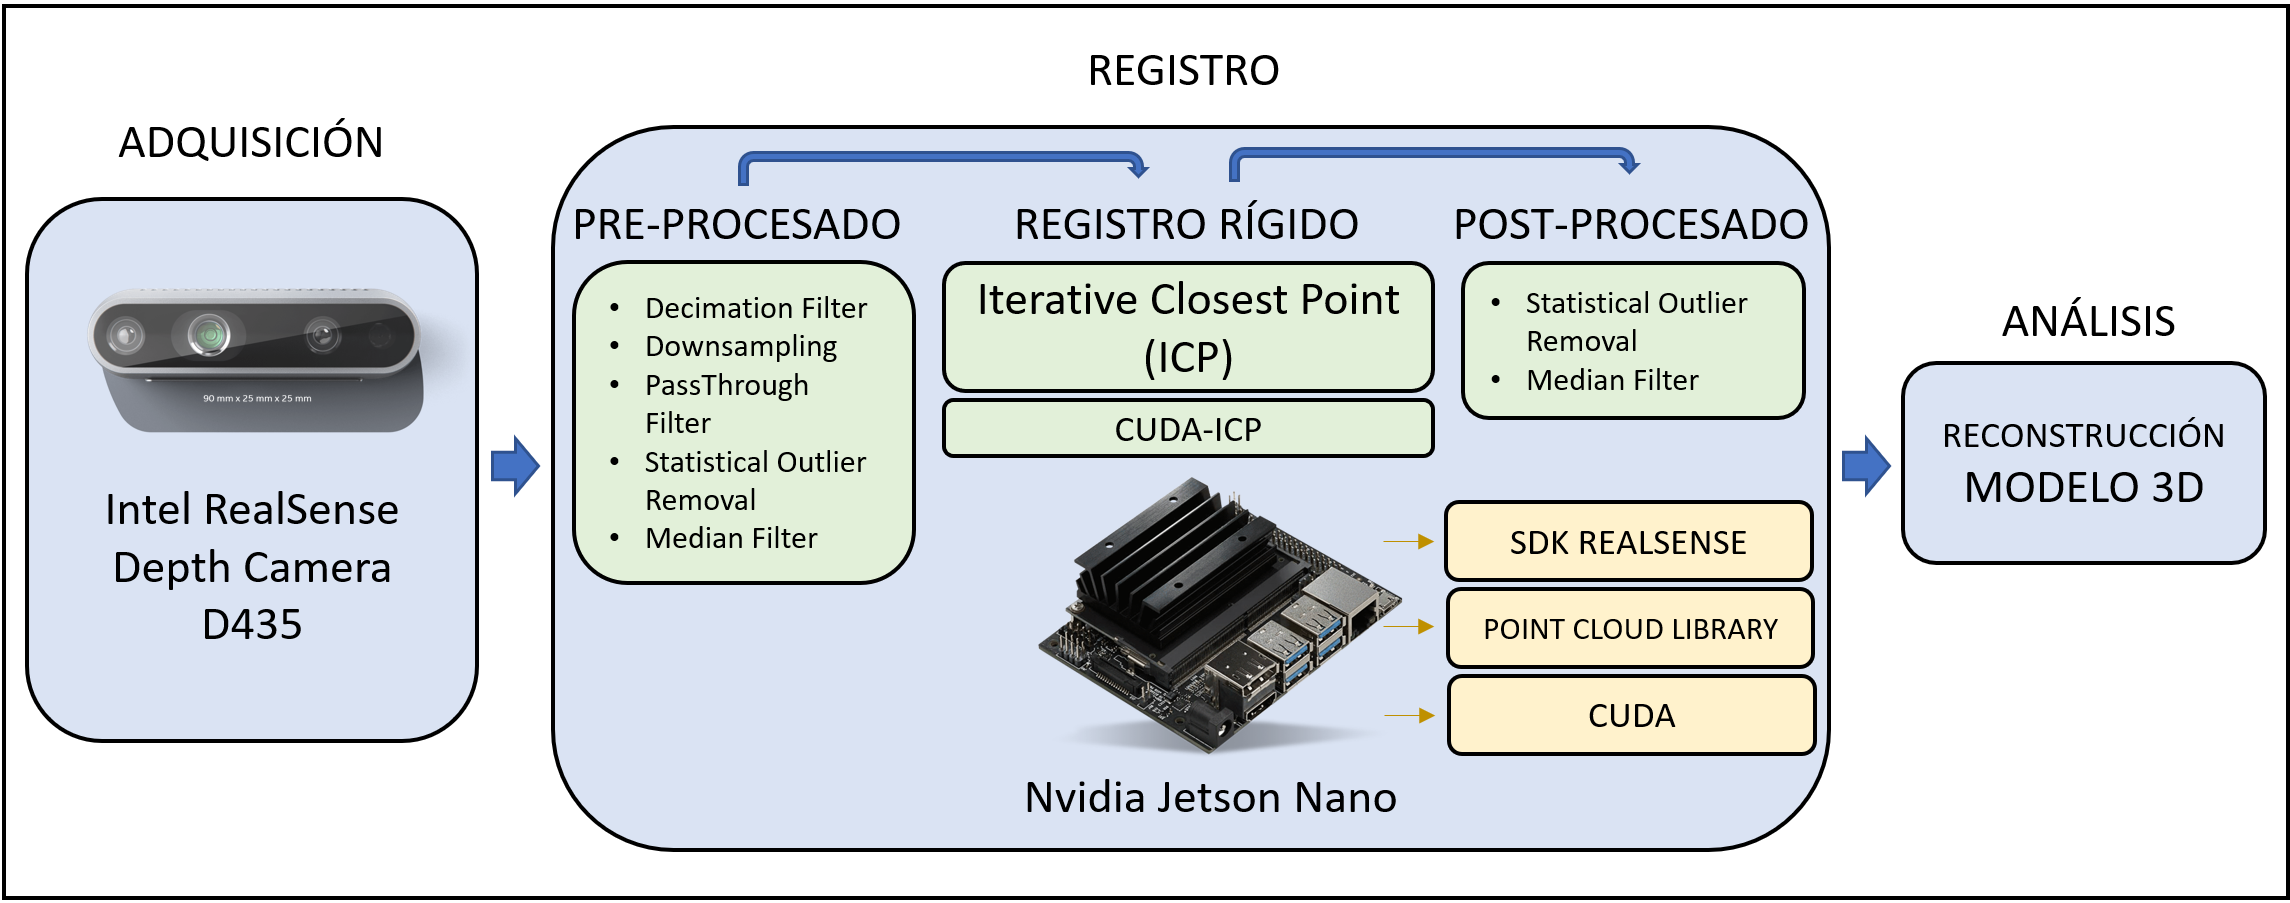
\includegraphics[width=\textwidth]{archivos/diagrama-propuesta-solucion.png}
    \caption{Diagrama de la propuesta e implementación de los módulos del sistema.}
    \label{fig:diagrama-propuesta-solucion}
\end{figure}

A continuación, durante este capítulo desarrollaremos cada una de las partes del diagrama explicando las cosas implementadas y el funcionamiento de cada uno de los módulos.

\section{Adquisición de datos}

Nuestro sistema de reconocimiento \gls{3d} consta del sensor Intel RealSense D435 conectado directamente a través de un puerto USB 3.0 al dispositivo Nvidia Jetson Nano.

Durante la fase de adquisición, el objetivo será realizar capturas RGBD a un modelo a través del sensor Intel RealSense D435.
Para ello, el sensor deberá estar fijo y el modelo deberá estar situado en el centro de la imagen para una mayor nitidez en las capturas.
El sensor realizará capturas constantemente y consecutivamente, mientras el modelo rota 360º poco a poco.
De esta forma, obtendremos muchas capturas desde distintos ángulos del modelo que posteriormente se procesarán para ser alineadas y reconstruir el modelo completamente en \gls{3d}.

Por tanto, será importante tener en cuenta la frecuencia de capturación del sensor, ya que cuanto mayor frecuencia, más rápido capturará al modelo, y menor será el ángulo de rotación entre cada una de las capturas.
Esto quiere decir que la distancia entre los puntos de dos capturas consecutivas será muy pequeña, y facilitará la tarea del registro con el algoritmo \gls{icp}.

El sensor Intel RealSense D435 es capaz de capturar a una frecuencia de hasta 30Hz en modo RGBD.
Realmente esto es más que suficiente, ya que 30Hz quiere decir que es capaz de capturar 30 imágenes en un segundo.
Hemos definido que cuanto más rápido se realicen las capturas es mejor, pero tanta velocidad realmente puede llegar a ser perjudicial, debido a que a esa frecuencia pueden llegar a realizarse cientos de capturas hasta que el modelo haya terminado de rotar 360º, haciendo que aumente el peso de trabajo a procesar debido a la enorme cantidad de datos.

Por ello, es necesario encontrar un punto medio. Como la frecuencia del sensor es mayor a las capturas que realmente queremos obtener por segundo, limitaremos la velocidad a la que se realizan las capturas introduciendo por parámetro un valor que indique cada cuanto realizar la captura.

Inicialmente y para testear, está bien separar la fase de adquisición de todas las capturas de la fase de registro. Sin embargo, se ha añadido una opción para funcionar de forma paralela e ir obteniendo el resultado a la vez que se realiza la adquisición total del modelo.
Es decir, una vez se hayan realizado la primera y segunda captura, estas serán enviadas para procesar el registro en otro hilo y, de forma concurrente, seguimos realizando la adquisición de nuevas capturas mientras el modelo está rotando.

\section{Pre-procesado}

Tras obtener la captura del modelo en la fase de adquisición, la captura se envía a la fase de pre-procesado donde se le aplicarán los filtros ya mencionados en apartados anteriores para reducir ruido y facilitar el procesamiento en la fase de registro.

El primer filtro a aplicar será el filtro diezmado (Decimal Filter). Este filtro realmente viene aplicado desde la fase de adquisición debido a que el filtro está integrado en la librería de RealSense desde la cual realizamos la captura, y se utiliza en el mismo proceso donde guardamos los datos y los enviamos al pre-procesado.
El filtro finalmente lo que consigue es una reducción de muestreo, como un downsampling, reduciendo el peso de la nube de puntos sin perjudicar demasiado la calidad, y facilitando las operaciones que se realizan dentro del algoritmo \gls{icp} que se procesará posteriormente.

Seguidamente al filtro de reducción de muestreo, se aplica el filtro ``Statistical Outlier Removal'' que nos permitirá deshacernos de los puntos atípicos que se encuentren más alejados del modelo en sí. Estos puntos normalmente son ruido por el borde del modelo que se genera en la fase de adquisición.
En la Figura \ref{fig:ejemplo-statistical-outlier-removal} podemos ver un ejemplo de aplicación de este filtro sobre un modelo \gls{3d}.

\begin{figure}[h]
    \centering
    \begin{subfigure}[t]{0.33\textheight}
    	\centering
        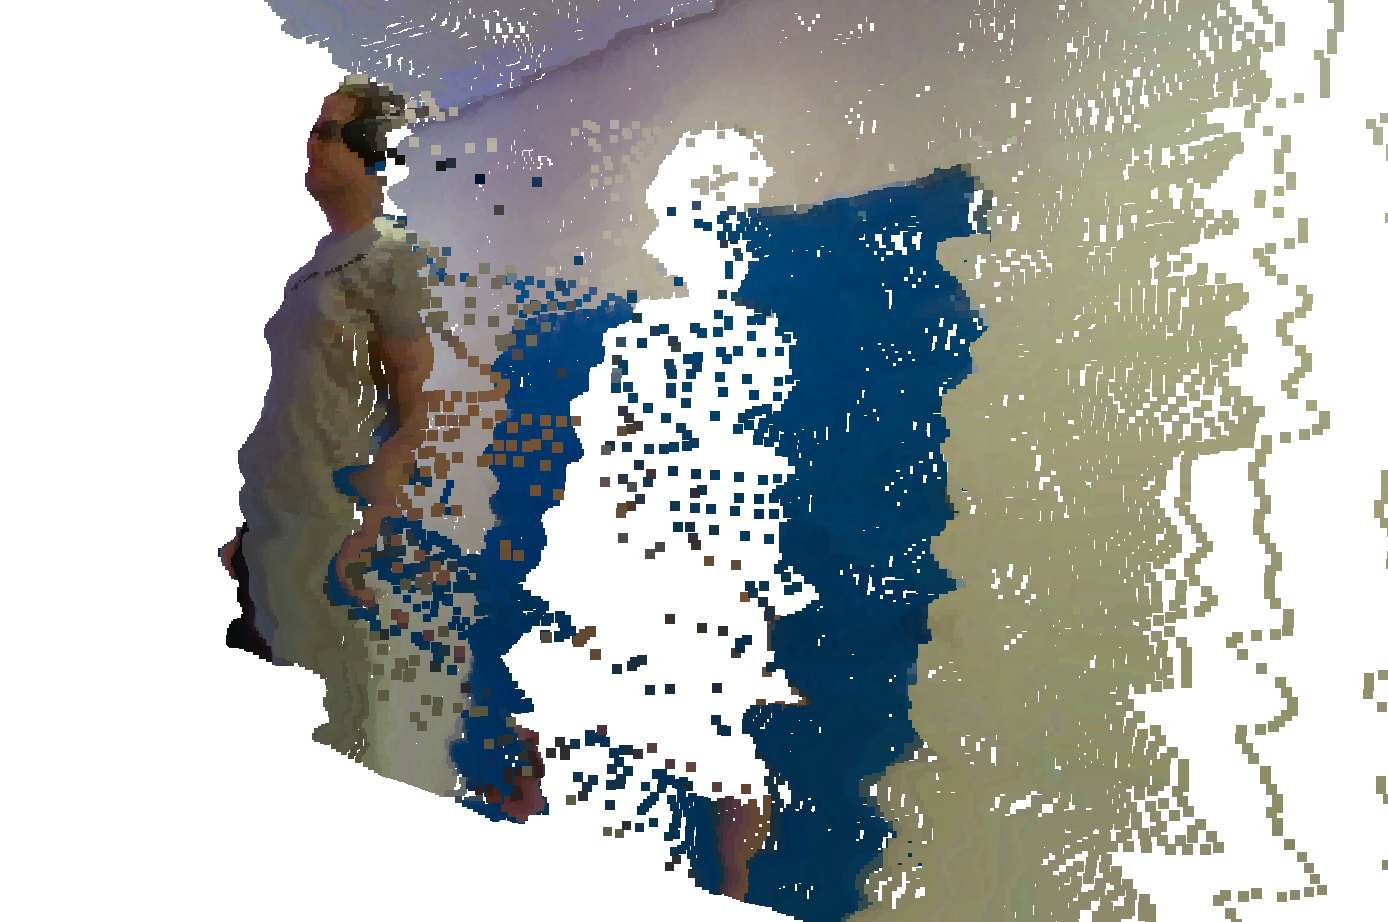
\includegraphics[height=4.5cm]{archivos/ejemplo-statistical-outlier-removal-original-2.png}
        \caption{Nube de puntos original.}
    \end{subfigure}
    \begin{subfigure}[t]{0.33\textheight}
    	\centering
        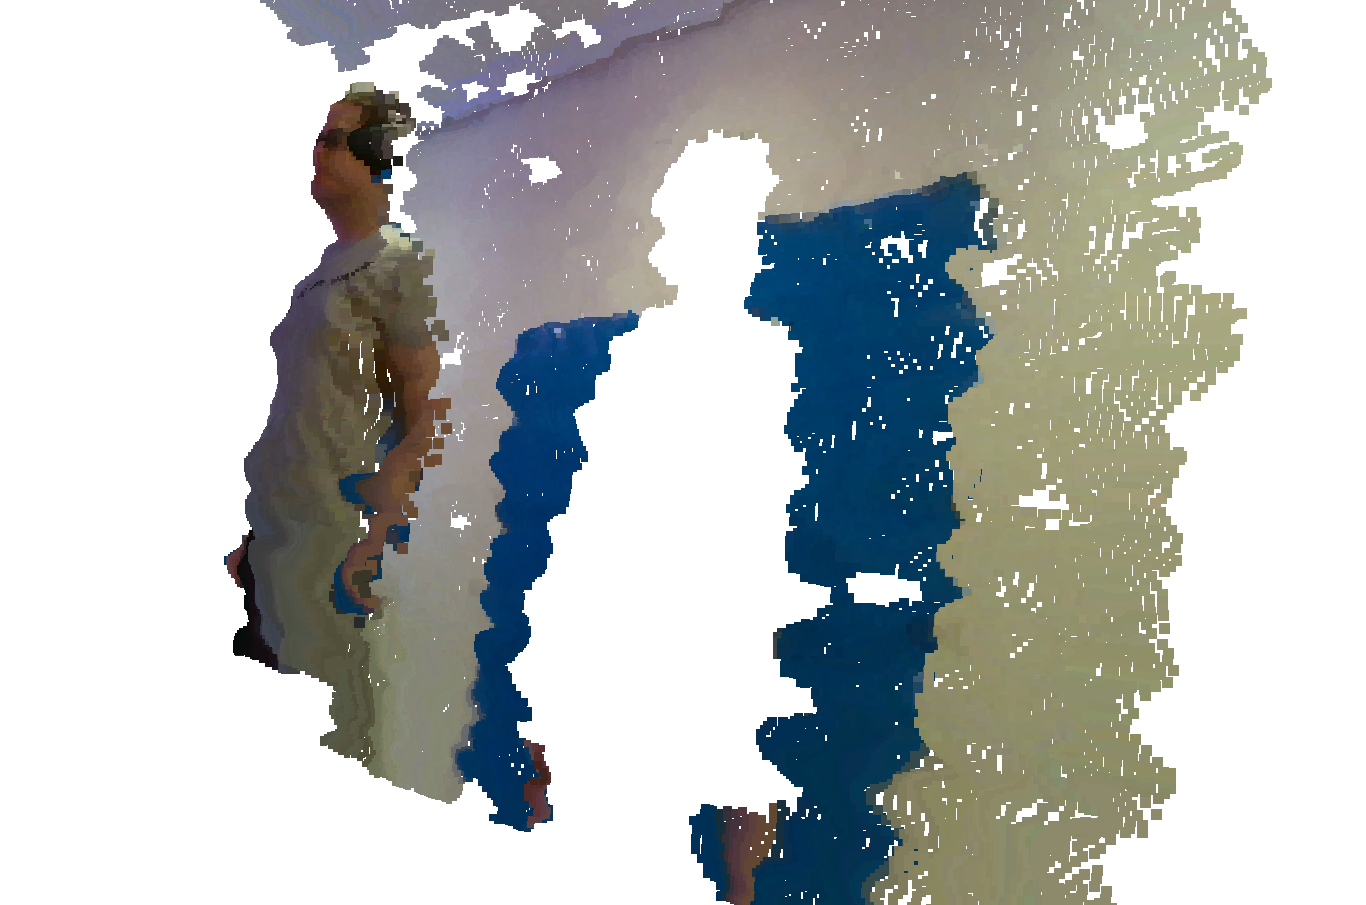
\includegraphics[height=4.5cm]{archivos/ejemplo-statistical-outlier-removal-filtro-2.png}
        \caption{Nube de puntos con filtro aplicado.}
    \end{subfigure}
    \caption{Ejemplo de filtro Statistical Outlier Removal aplicado.}
    \label{fig:ejemplo-statistical-outlier-removal}
\end{figure}

Por último, se aplica el filtro de la mediana, que permite homogeneizar el modelo \gls{3d} reduciendo el ruido que hay en el propio modelo, aplanandolo ligeramente.
% En la Figura \ref{fig:ejemplo-filtro-mediana} podemos ver un ejemplo de aplicación de este filtro sobre un modelo \gls{3d}.

% \begin{figure}[h]
%     \centering
%     \begin{subfigure}[t]{0.33\textheight}
%     	\centering
%         % 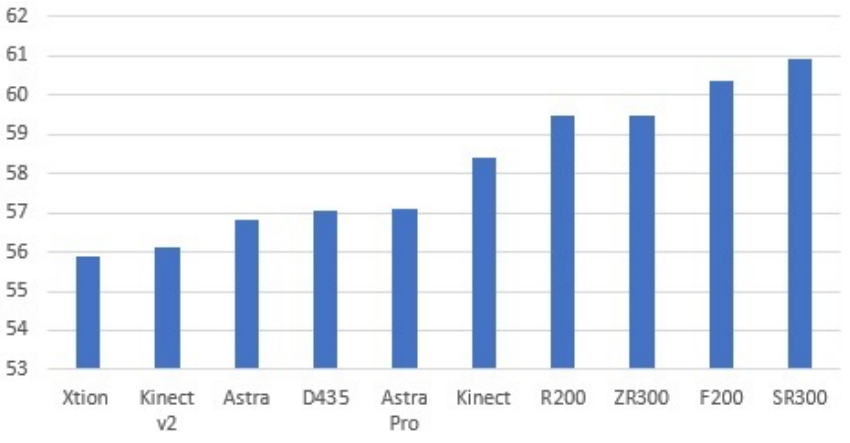
\includegraphics[height=3.5cm]{archivos/comparacion-sensores-recorrido1.png}
%         % la imagen debe ser con los puntos cercanos pero que sobre mucho de ambos lados sin corresponder, para mostrar que con el limite de maxima distancia esos puntos se ignorarian
%         \missingfigure{}
%         \caption{Nube de puntos original.}
%     \end{subfigure}
%     \begin{subfigure}[t]{0.33\textheight}
%     	\centering
%         % 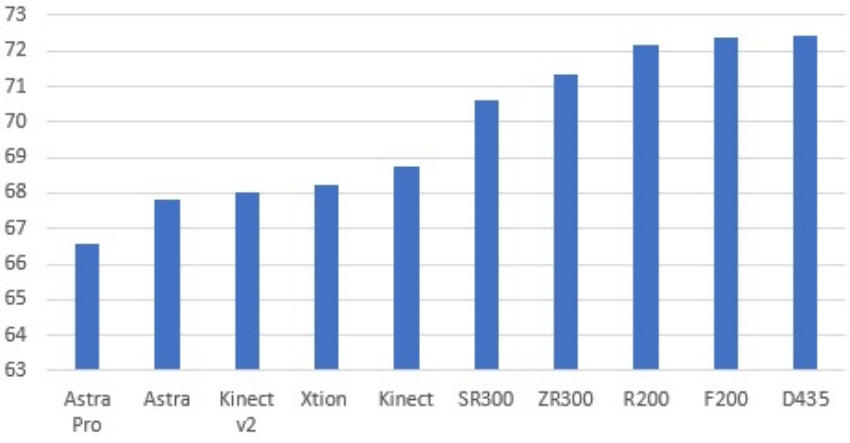
\includegraphics[height=3.5cm]{archivos/comparacion-sensores-recorrido2.png}
%         \missingfigure{}
%         \caption{Nube de puntos con filtro aplicado.}
%     \end{subfigure}
%     \caption{Ejemplo de filtro mediana aplicado.}
%     \label{fig:ejemplo-filtro-mediana}
% \end{figure}

\section{Registro}

En la fase de registro es donde conseguiremos reconstruir, poco a poco, el modelo en \gls{3d} por completo.
Para esta fase, nuestra solución consta de dos implementaciones sobre las que se han hecho las pruebas.
En una de ellas se utiliza el algoritmo \gls{icp} de la librería \gls{pcl}, y en la otra se utiliza CUDA-ICP, que se trata de una implementación en \gls{cuda} sobre el algoritmo \gls{icp} de la librería \gls{pcl} también.
No obstante, el uso de ambas implementaciones es el mismo, ambas reciben un modelo y una escena como entrada, y devuelven la matriz de transformación a aplicar sobre la escena.

Cabe destacar que no se hace uso de ningún algoritmo de grano grueso para un primer aproximamiento de la escena al modelo, como se ha explicado en la sección \ref{sec:metodos-de-registro}.
Aunque es muy común utilizar RANSAC-ICP para estos procesos de reconstrucción de modelos \gls{3d}, el caso de nuestro proyecto se encuentra muy bien definido en un entorno y unas características concretas que hacen que no sea necesario utilizar estos métodos como apoyo.
Debido a que la fase de adquisición es lo suficientemente rápida, la distancia entre cada par consecutivo de capturas es muy pequeña, lo cual nos permite procesar el método \gls{icp} sin necesidad de aproximar la escena previamente.

Por tanto, esta fase recibe dos nubes de puntos ya pre-procesadas, una de ellas será el modelo, y la otra será la escena.
En una primera iteración de esta solución, el algoritmo recibirá la captura 1 como la nube de puntos modelo, y la captura 2 como la nube de puntos escena.
Estas nubes de puntos son procesadas, obteniendo la matriz de transformación que hay que aplicar sobre la escena para que esta quede alineada con el modelo.
Seguidamente, transformamos la escena para que quede alineada con el modelo y juntamos ambas nubes de puntos, consiguiendo así una única nube de puntos que tenga la información de las capturas 1 y 2.
Nos guardamos la matriz de transformación obtenida para aplicarselo a las futuras escenas como matriz de transformación inicial.

En una segunda iteración de la solución, esta fase recibirá una nueva nube de puntos perteneciente a la captura 3, que será la nueva escena.
Por tanto, tendremos la nube de puntos modelo que constará de las capturas 1 y 2, y la nube de puntos escena que corresponde con la captura 3.
Previamente a procesar las nubes de puntos por el algoritmo \gls{icp}, se aplicará la matriz de transformación de la iteración anterior como transformación inicial para la captura 3, haciendo así que esta nube de puntos escena quede más próxima al modelo.
Ahora sí, las nubes de puntos serán procesadas por el algoritmo y obtendremos una nueva matriz de transformación que habrá que aplicar sobre la captura 3 para que quede alineada con el modelo.
Aplicaremos dicha matriz de transformación y nos la volveremos a guardar para la siguiente iteración, aunque realmente lo que haremos será multiplicarla con la matriz de transformación que ya teníamos de la iteración anterior, haciendo así que la futura captura 4 utilice como matriz de transformación el resultado de todas las matrices de transformación de las iteraciones anteriores.
En el diagrama de la Figura \ref{fig:diagrama-acumulacion-matriz-transformacion} podemos ver este proceso con un esquema.

\begin{figure}[h]
    \centering
    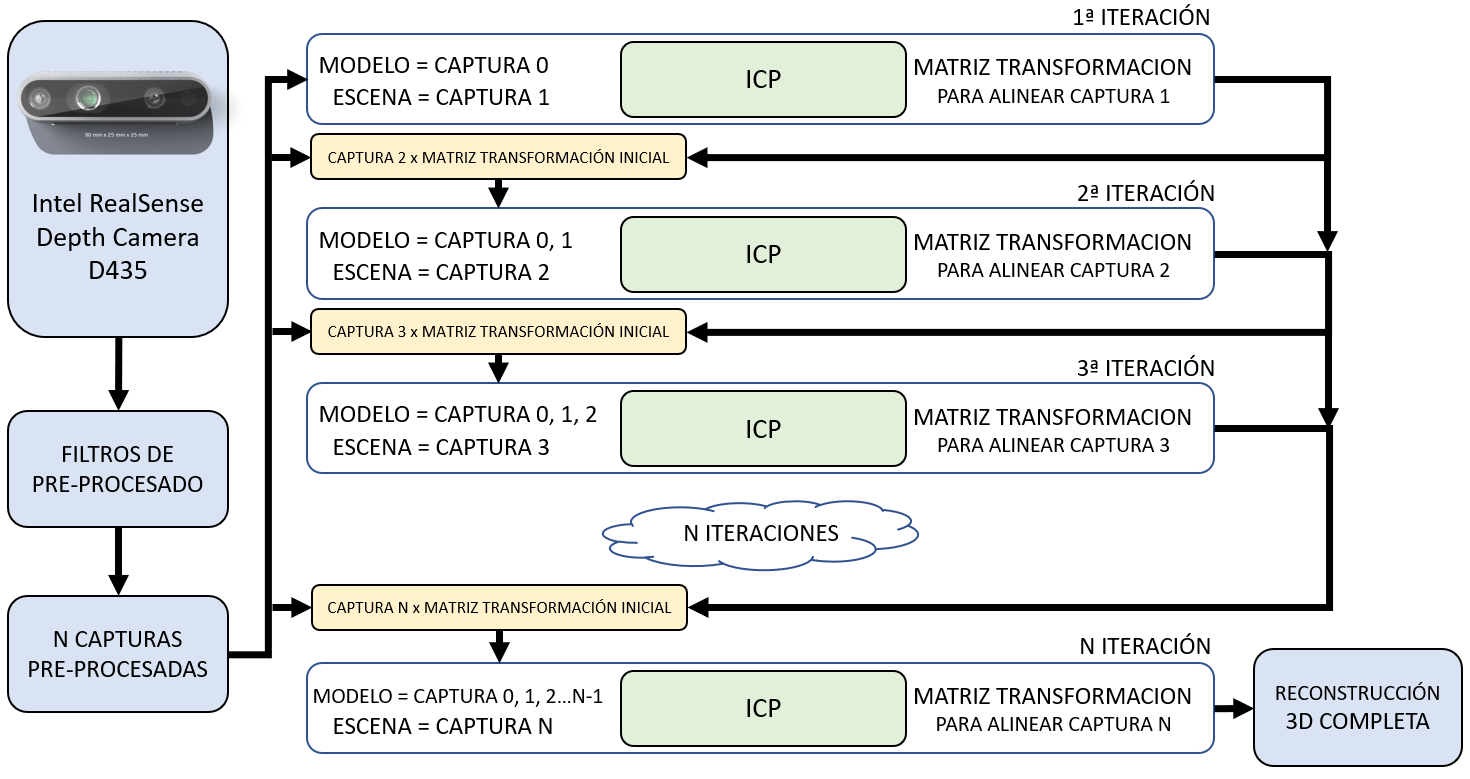
\includegraphics[width=\textwidth]{archivos/diagrama-acumulacion-matriz-transformacion.png}
    \caption{Diagrama de reconstrucción 3D acumulando matrices de transformación para cada nueva iteración.}
    \label{fig:diagrama-acumulacion-matriz-transformacion}
\end{figure}

\subsection{Posible refinamiento con CPD}

Como propuesta general, se puede hacer uso de un método de registro no rígido para corregir errores, como los producidos por el movimiento del cuerpo.
Concretamente se ha probado una pequeña implementación con el algoritmo \gls{cpd} explicado previamente en el apartado \ref{subsec:metodos-registro-no-rigido-cpd}.
La ventaja de este algoritmo es la posibilidad de utilizar el registro no rígido para corregir los errores de movimiento que se puedan haber producido durante la rotación 360º del cuerpo humano durante la fase de adquisición, ya que el cuerpo puede deformarse entre las capturas.
El algoritmo ha sido implementado de una manera similar a los otros dos, sin embargo no se contempla como solución final debido al largo tiempo de cómputo que emplea, no pudiendo proporcionar un resultado final.

\section{Post-procesado}

Tras finalizar la fase de registro y obtener el modelo final alineado y reconstruido, opcionalmente podemos utilizar la fase de post-procesado para aplicar unos filtros con la finalidad de reducir un poco el posible ruido que se haya podido generar durante la fase de registro.

Estos filtros serán el filtro ``Statistical Outlier Removal'' que se deshará de puntos atípicos lejanos a los bordes del modelo y el filtro de mediana, para aplanar y homogeneizar el modelo en sí.

\section{Análisis}

En esta última fase nos encontramos con una única nube de puntos, resultado de alinear todas las escenas con la primera nube de puntos de la fase de adquisición.

Esta nube de puntos la encontramos en un fichero con formato ``.ply'' que puede ser abierta por programas para visualizar nubes de puntos de modelos \gls{3d} como lo es MeshLab.
En la Figura \ref{fig:analisis-ejemplo-resultado} podemos ver un ejemplo de resultado en la fase de análisis.

\begin{figure}[h]
    \centering
    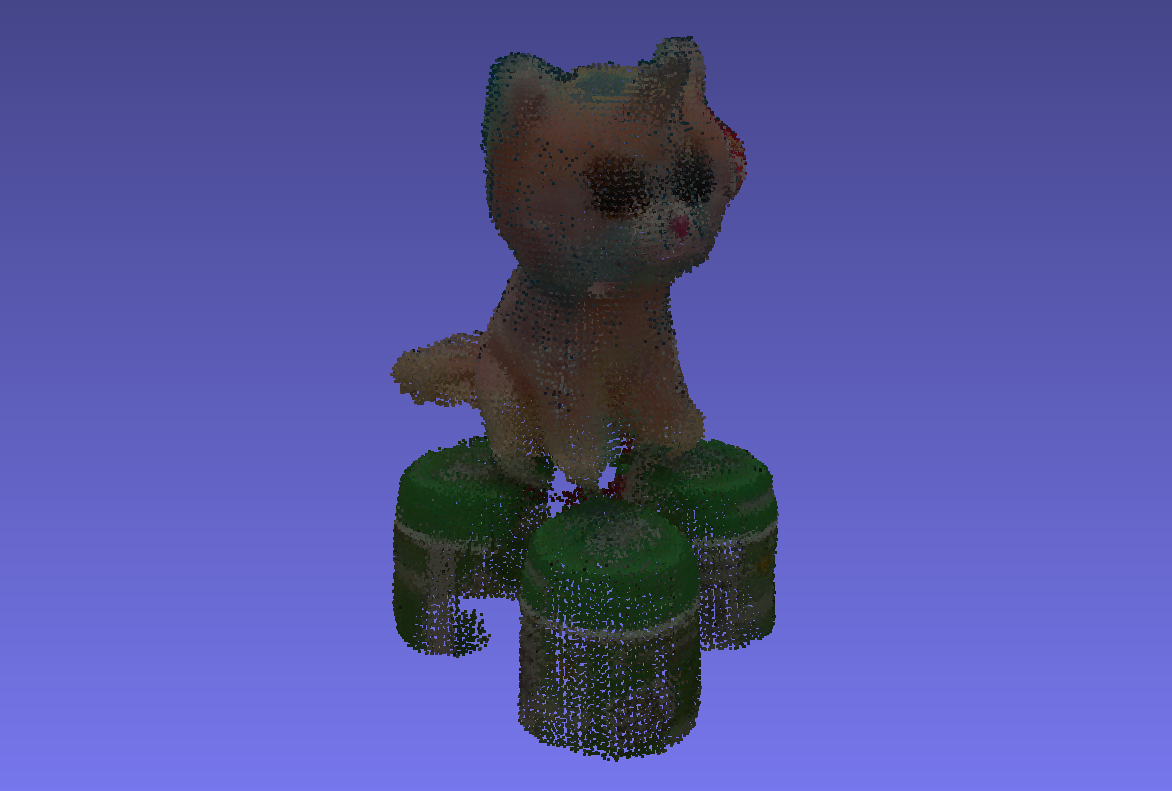
\includegraphics[width=\textwidth]{archivos/analisis-ejemplo-resultado.png}
    \caption{Ejemplo de modelo 3D en la fase de análisis.}
    \label{fig:analisis-ejemplo-resultado}
\end{figure}

Esta fase trata básicamente de visualizar el resultado para analizar posibles mejoras en la experimentación.

\chapter{Solución del proyecto en Jetson Nano}
\label{cap:solucion-proyecto}

En este capítulo detallaremos como se ha llevado a cabo la propuesta explicada en el capítulo anterior.
Aunque existen muchas soluciones, librerías y proyectos compartidos en Python que podrían facilitar el desarrollo de este proyecto, nos hemos decantado por utilizar C\texttt{++}, debido a que estoy algo más familiarizado con esta tecnología y destaca por ser más rápida, con mejor rendimiento.
Todo eso a pesar de haber desarrollado un código bastante simple limitándonos a utilizar librerías existentes, C\texttt{++} ofrece la posibilidad de meterse más a bajo nivel para poder optimizar mejor el código, entrando más en el grano fino. Por lo que C\texttt{++} nos ha parecido una propuesta inicial interesante.

\section{Integración del Software. Dependencias}

En primer lugar, explicaremos todo el software que ha sido necesario instalar, tanto para las dependencias con el proyecto C\texttt{++} como el software necesario para hacer que el dispositivo Nvidia Jetson Nano funcionase a la perfección con el sensor Intel RealSense D435.

\subsection{Sistema Operativo. Ubuntu 18.04}

La fuente de este sistema operativo se puede obtener desde la página oficial de Nvidia, a través de \href{https://developer.nvidia.com/embedded/jetpack}{JetPack SDK} donde nos guían para llevar a cabo la instalación.
NVIDIA JetPack SDK es la solución más completa para un entorno de desarrollo completo en el desarrollo acelerado por hardware. Todos los módulos y kits para desarrolladores de Jetson Nano son compatibles con JetPack SDK.
JetPack SDK incluye Jetson Linux Driver Package con cargador de arranque, kernel de Linux, entorno de escritorio Ubuntu y un conjunto completo de bibliotecas para la aceleración de computación GPU, multimedia, gráficos y visión por computadora.

El último SDK disponible para el dispositivo Nvidia Jetson Nano es el JetPack 4.6.1, cuyo sistema operativo es Ubuntu 18.04 con versión \gls{cuda} 10.2.
El SDK JetPack 5.0 utiliza el sistema operativo de Ubuntu 20.04 con versión \gls{cuda} 11.4, pero actualmente no está disponible para Nvidia Jetson Nano, solo para modelos superiores.

\subsection{CMake. Compilador C\texttt{++}}

Como se ha mencionado anteriormente, hemos decidido elaborar el proyecto en el lenguaje C\texttt{++}. Para ello, se ha construido un proyecto utilizando CMake.

CMake es una familia de herramientas diseñada para construir, probar y empaquetar software.
Se utiliza para controlar el proceso de compilación del software usando ficheros de configuración sencillos e independientes de la plataforma.
Gracias al uso de CMake, el proyecto queda fácilmente configurado, encargándose de enlazar todas las dependencias que el proyecto necesite.
Por tanto, será necesario tener instaladas todas las herramientas necesarias para la correcta ejecución de CMake.

Además, será necesario tener instalado el compilador de C\texttt{++} para poder compilar el proyecto. El compilador instalado en el dispositivo Nvidia Jetson Nano GCC versión Ubuntu/Linaro 7.5.0-3ubuntu1~18.04.

\subsection{SDK RealSense}

Para la instalación del SDK de RealSense se ha utilizado un script que ha facilitado la instalación del mismo.
En el GitHub de \href{https://github.com/JetsonHacksNano/installLibrealsense}{installLibrealsense} podemos encontrar un script que se encarga de añadir al repositorio del gestor de paquetes las fuentes necesarias y de instalar todos los paquetes necesarios de forma automática.
Por tanto, tras clonar dicho proyecto y ejecutar el script ``./installLibrealsense.sh'' tendremos instalado por completo el SDK de RealSense.

Una vez instalado el software, podremos utilizar la aplicación RealSense Viewer para visualizar la cámara tanto en \gls{2d} como en \gls{3d}.
También podremos compilar sin problemas añadiendo las dependencias necesarias en el fichero CMakeLists.txt, como se muestra en el Código \ref{lst:dependencia-realsense}.

\begin{lstlisting}[language={C++}, caption={Dependencia CMakeLists: RealSense Library}, label={lst:dependencia-realsense}]
    # RealSense Library
    find_package(realsense2 REQUIRED)
    include_directories(include ${realsense_INCLUDE_DIR})
    target_include_directories(main PRIVATE ${realsense_INCLUDE_DIR})
    target_link_libraries(main ${realsense2_LIBRARY})
\end{lstlisting}

\subsection{Point Cloud Library (PCL)}

\gls{pcl} es una biblioteca de código abierto de algoritmos para tareas de procesamiento de nubes de puntos y procesamiento de geometría 3D, como ocurre en la visión tridimensional por computadora.
La biblioteca contiene algoritmos para filtrado, estimación de características, reconstrucción de superficies, registro 3D, ajuste de modelos, reconocimiento de objetos y segmentación.
Cada módulo se implementa como una biblioteca más pequeña que se puede compilar por separado.
PCL tiene su propio formato de datos para almacenar nubes de puntos: \gls{pcd}, pero también permite cargar y guardar conjuntos de datos en muchos otros formatos, como \gls{ply}.
También está escrito en C\texttt{++} y publicado bajo la licencia BSD.

Esta librería es muy interesante y la utilizamos tanto para aplicar filtros de pre-procesado y post-procesado, como para el método de registro \gls{icp}.

Además de tener instalada la librería, debe estar incluida como dependencia en el fichero CMakeLists.txt del proyecto de la forma que se muestra en el Código \ref{lst:dependencia-pcl}.

\begin{lstlisting}[language={C++}, caption={Dependencia CMakeLists: Point Cloud Library}, label={lst:dependencia-pcl}]
    # Point Cloud Library
    find_package(PCL 1.8 REQUIRED)
    include_directories(${PCL_INCLUDE_DIRS})
    link_directories(${PCL_LIBRARY_DIRS})
    add_definitions(${PCL_DEFINITIONS})
    target_link_libraries(main ${PCL_COMMON_LIBRARIES} ${PCL_IO_LIBRARIES} ${PCL_FILTERS_LIBRARIES})
\end{lstlisting}

\subsection{CUDA. CUDA-ICP.}

Gracias a haber instalado el sistema operativo con JetPack SDK, toda la librería de \gls{cuda} 10.2 ya viene instalada por defecto en el sistema operativo, por lo que solamente será necesario incluir como dependencia en el fichero CMakeLists.txt del proyecto de la forma que se muestra en el Código \ref{lst:dependencia-cuda}.

\begin{lstlisting}[language={C++}, caption={Dependencia CMakeLists: CUDA}, label={lst:dependencia-cuda}]
    # CUDA Library
    find_package(CUDA 10.2 REQUIRED)
    include_directories(${CUDA_INCLUDE_DIRS})
    target_link_libraries(main ${CUDA_LIBRARIES})
\end{lstlisting}

Además, encontramos un repositorio oficial de Nvidia que nos ofrece una implementación de \gls{icp} en \gls{cuda}.
Este repositorio llamado \href{https://github.com/NVIDIA-AI-IOT/cuda-pcl}{CUDA-PCL} contiene diversas implementaciones en \gls{cuda} de distintos algoritmos de la librería \gls{pcl}, entre ellos CUDA-ICP.

Nos hemos descargado de ahí la implementación \gls{icp} y la hemos importado en nuestro proyecto con las líneas en el fichero CMakeLists.txt que se muestran en el Código \ref{lst:dependencia-cuda-icp}.

\begin{lstlisting}[language={C++}, caption={Dependencia CMakeLists: CUDA-ICP}, label={lst:dependencia-cuda-icp}]
    # CUDA ICP Local Library
    target_include_directories(main PRIVATE ${CMAKE_CURRENT_SOURCE_DIR})
    add_library(libcudaicp SHARED IMPORTED)
    set_target_properties(libcudaicp PROPERTIES IMPORTED_LOCATION ${CMAKE_CURRENT_SOURCE_DIR}/lib/libcudaicp.so)
    target_link_libraries(main libcudaicp)
\end{lstlisting}

\subsection{JsonCpp}

JsonCpp es una librería que permite leer y escribir fácilmente ficheros Json en C\texttt{++}.
Esta librería no cumple ninguna función esencial para el proceso de reconstrucción de un modelo \gls{3d}, pero es muy útil ya que usamos un fichero .json donde definimos todos los parámetros que la aplicación debe tener en cuenta a la hora de ejecutarse.
Por tanto es una dependencia necesaria si se pretende compilar el proyecto tal y como se encuentra ahora mismo, ya que los parámetros se leen de un fichero .json.

Además de tener instalada la librería, debe estar incluida como dependencia en el fichero CMakeLists.txt del proyecto de la forma que se muestra en el Código \ref{lst:dependencia-jsoncpp}.

\begin{lstlisting}[language={C++}, caption={Dependencia CMakeLists: JsonCpp}, label={lst:dependencia-jsoncpp}]
    # JsonCpp Library
    find_package(PkgConfig REQUIRED)
    pkg_check_modules(JSONCPP jsoncpp)
    link_libraries(${JSONCPP_LIBRARIES})
    target_link_libraries(main ${JSONCPP_LIBRARIES})
    configure_file(parameters.json parameters.json COPYONLY)
\end{lstlisting}

\section{Desarrollo de la solución}

Tras la instalación de todo el software necesario, explicaremos detalladamente los fragmentos más relevantes del código desarrollado, siguiendo el esquema explicado en el capítulo \ref{cap:propuesta-de-solucion}, Figura \ref{fig:diagrama-propuesta-solucion}.

El programa consiste en una aplicación de consola con un pequeño menú numerado con las distintas opciones a realizar, desde la ejecución total de la reconstrucción pasando por todas las fases automáticamente tanto para la implementación de \gls{icp} de \gls{pcl} como para la implementación de CUDA-ICP, hasta la ejecución de cada una de las fases por separado, con finalidad de analizar y experimentar mejor con los resultados.

Debido a que la ejecución del algoritmo conlleva variables que no son fijas para distintos casos de uso, se ha creado un fichero json para poder personalizar los parámetros de ejecución.
A la hora de lanzar el programa, lo primero que se hace es leer el fichero json llamado ``parameters.json'' que contiene la siguiente información que se muestra en el fragmento de Código \ref{lst:parametros-aplicacion}.

\begin{lstlisting}[language={C++}, caption={Parámetros de la aplicación}, label={lst:parametros-aplicacion}]
    {
        "DataPath" : "/home/edgar/tfg/Code Solutions/JetsonNano/.data/",
        "RealSenseCaptureTotalTime_ms" : 27500,
        "RealSenseCaptureTimingBetweenCaptures_ms" : 500,
        "NumberOfCaptureFiles" : 52,
        "ResizeCenterDistance_m" : 0.63,
        "ResizeCaptureBottom_m" : 0.47,
        "ResizeCaptureTop_m" : 0.25,
        "ResizeCaptureLeft_m" : 0.5,
        "ResizeCaptureRight_m" : 0.5,
        "ResizeCaptureBehind_m" : 0.35,
        "ResizeCaptureFront_m" : 0.4,
        "ICP_Iterations" : 200,
        "ICP_MaxCorrespondenceDistance" : 0.015
    }
\end{lstlisting}

``DataPath'' especifica la ruta donde se van a guardar y tratar toda la información que sea necesaria.
Por ejemplo, si ejecutamos la fase de adquisición por separado, se guardarán ahí los ficheros para poder ser procesados posteriormente por otra fase.
El resto de parámetros los iremos viendo en este capítulo a medida que se va explicando el código.

\subsection{Adquisición de datos}

Para la fase de adquisición necesitaremos conectarnos a la cámara a través del SDK de RealSense. Para ello, inicializaremos las variables que podemos ver a continuación en el Código \ref{lst:inicializacion-adquisicion}.
``rs2::pipeline'' es la clase que se encarga de gestionar el sensor y que nos permitirá recibir los frames que está captando.
``rs2::pointcloud'' nos permitirá gestionar los frames que recibimos del sensor para convertirlos a nubes de puntos y de esta manera poder procesar el algoritmo posteriormente.
Por último, ``decimation\_filter'' se encargará de aplicar el filtro de diezmado a los frames de profundidad capturados por el sensor antes incluso de convertirlos a nubes de puntos.
Como se ha mencionado en el Capítulo \ref{cap:propuesta-de-solucion}, este es el único filtro que se ejecuta antes de la fase de pre-procesamiento, ya que se hace en el momento de la adquisición del frame.

Además de la inicialización también podemos observar un bucle inicial que se encarga de crear autoexposición en la imagen, de forma que las primeras capturas se realicen correctamente y no aparezcan oscuras o con ruido.

\begin{lstlisting}[language={C++}, caption={Inicialización del sensor RealSense D435 para la adquisición de datos}, label={lst:inicializacion-adquisicion}]
    rs2::decimation_filter decimation_filter;
    rs2::pointcloud pointcloud;
    rs2::pipeline pipe;
    pipe.start();

    std::cout << "Capturando 30 frames para autoexposicion..." << std::endl;
    for (auto i = 0; i < 30; i++) pipe.wait_for_frames();
\end{lstlisting}

A continuación, en el Código \ref{lst:bucle-adquisicion} tenemos un bucle cuya duración estará establecida por parámetro a través de la variable ``RealSenseCaptureTotalTime\_ms''.
Con la variable ``RealSenseCaptureTimingBetweenCaptures\_ms'' podemos establecer el tiempo de espera entre frame y frame que también estará establecido por parámetro.

En este bucle guardaremos los frames que recibe la cámara, aplicando el filtro de diezmado y mapeandolos a nube de puntos con RGB. Una vez obtenemos la nube de puntos, se guarda en un vector que será tratado posteriormente.

\begin{lstlisting}[language={C++}, caption={Bucle para adquisición de los datos con el sensor RealSense D435}, label={lst:bucle-adquisicion}]
    while (time < RealSenseCaptureTotalTime_ms)
    {
        std::this_thread::sleep_for(std::chrono::milliseconds(RealSenseCaptureTimingBetweenCaptures_ms));
       
        auto fs = pipe.wait_for_frames();
        auto depth = fs.get_depth_frame();
        auto color = fs.get_color_frame();

        depth.keep();
        color.keep();
        depths.push_back(depth);
        colors.push_back(color);
        pointcloud.map_to(colors[i]);
        depths[i] = decimation_filter.process(depths[i]);
        depths[i].keep();
        points.push_back(pointcloud.calculate(depths[i]));
        points[i].keep();

        i++;
    }
\end{lstlisting}

Finalmente, tenemos dos maneras de continuar con los datos. Por una parte, en el fragmento de Código \ref{lst:guardar-nubes-puntos-adquisicion} podemos ver que guarda todas las nubes de puntos almacenadas en el vector en fichero ``.ply'' para su posterior tratamiento.
Esto es útil cuando queremos separar la ejecución del programa en sus diferentes fases, ya que nos permite analizar la adquisición antes de continuar con el procesamiento de los datos.

\begin{lstlisting}[language={C++}, caption={Guardar las nubes de puntos en un fichero de datos}, label={lst:guardar-nubes-puntos-adquisicion}]
    for (i = 0; i < depths.size(); i++)
    {
        std::stringstream filename;
        filename << DataPath << "adquisitionFromRealSense/" << i << ".ply";
        points[i].export_to_ply(filename.str(), colors[i]);
    }
\end{lstlisting}

Sin embargo, cuando sabemos que el método de adquisición funciona correctamente, tenemos la alternativa de guardar las nubes de puntos directamente en memoria convirtiéndolas en nubes de puntos compatibles con la librería \gls{pcl} como podemos ver en el Código \ref{lst:tranformar-nubes-puntos-adquisicion}.

\begin{lstlisting}[language={C++}, caption={Conversión de una nube de puntos de la librería RealSense a una nube de puntos de PCL}, label={lst:tranformar-nubes-puntos-adquisicion}]
    for (i = 0; i < depths.size(); i++)
    {
        pcl::PointCloud<pcl::PointXYZRGB>::Ptr cloud_in = parseToPCLRGB(points[i], colors[i]);
        applyPreprocessingFilterTo(cloud_in);
    }
\end{lstlisting}

\subsection{Pre-procesado}

Como se ha visto a lo largo del \gls{tfg}, a pesar de estar enfocado en la reconstrucción de cuerpos humanos, también se han procesado objetos debido a su mayor facilidad ya que son cuerpos rígidos.
La adquisición de datos de estos objetos han sido tomadas desde un ángulo superior, por lo que para este tipo de datos se utiliza una matriz de rotación de 30º en el eje X para que la nube de puntos quede bien alineada inicialmente. En la subfigura \ref{fig:preprocesamiento-sin-rotar} podemos ver la nube de puntos original y en la subfigura \ref{fig:preprocesamiento-rotado} la misma nube de puntos perfectamente orientada respecto al eje X.
Para ello se usa la matriz de rotación que se muestra en el Código \ref{lst:rotacion-preprocesamiento} sobre la nube de puntos adquirida en la fase de adquisición.

\begin{figure}[h]
    \centering
    \begin{subfigure}[t]{0.33\textheight}
    	\centering
        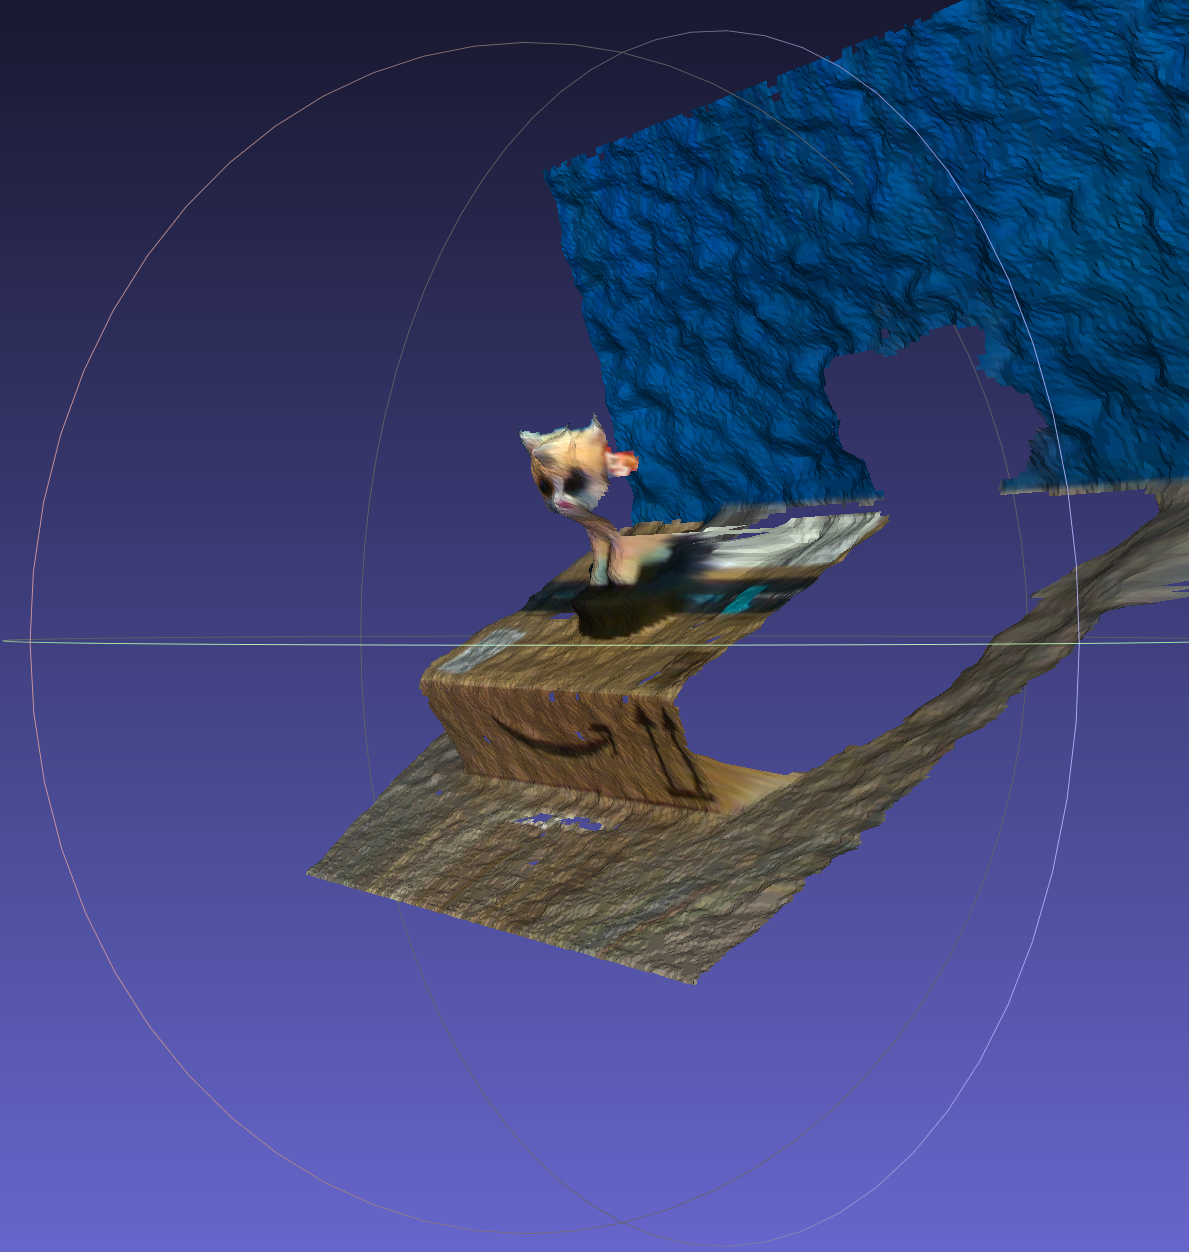
\includegraphics[height=4cm]{archivos/preprocesamiento-sin-rotar.png}
        \caption{Nube de puntos original con un ángulo de 30º desde arriba.}
        \label{fig:preprocesamiento-sin-rotar}
    \end{subfigure}
    \begin{subfigure}[t]{0.33\textheight}
    	\centering
        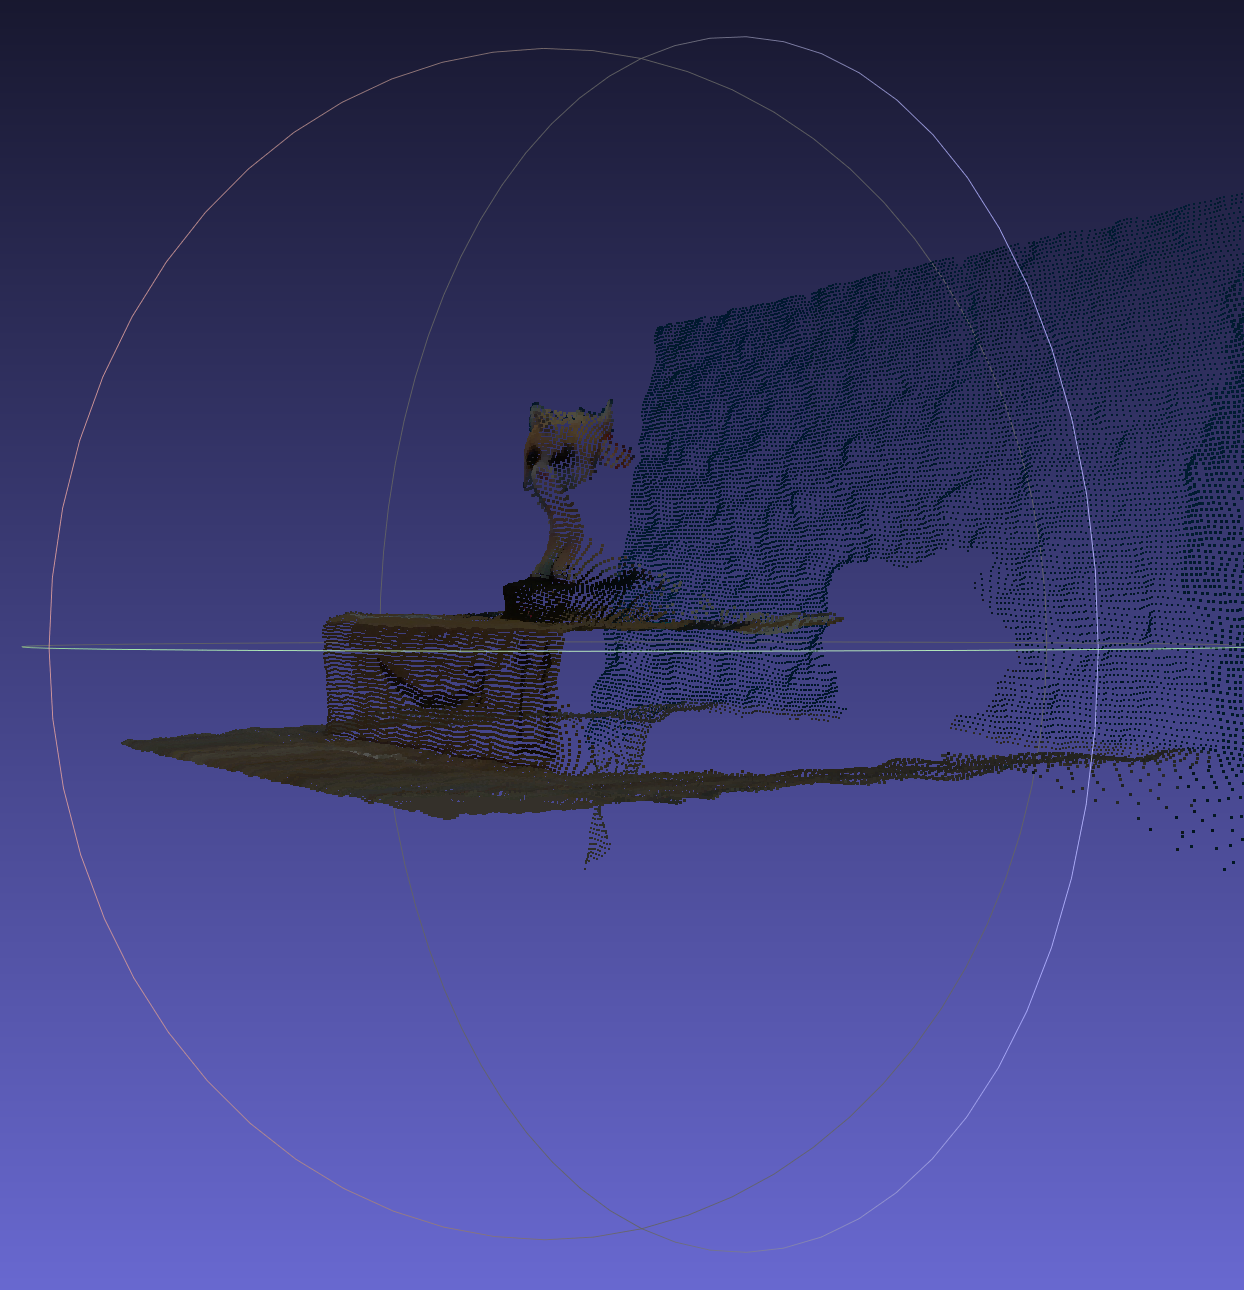
\includegraphics[height=4cm]{archivos/preprocesamiento-rotado.png}
        \caption{Nube de puntos rotada.}
        \label{fig:preprocesamiento-rotado}
\end{subfigure}
    \caption{Ejemplo de rotación en el pre-procesamiento de datos para dejar la nube de puntos alineada con el eje X.}
    \label{fig:preprocesamiento-rotar}
\end{figure}

\begin{lstlisting}[language={C++}, caption={Rotación en fase de pre-procesamiento de la nube de puntos}, label={lst:rotacion-preprocesamiento}]
    Eigen::Matrix4f transformation_matrix = Eigen::Matrix4f::Identity();
    double theta = degreesToRadians(-30);
    transformation_matrix(1, 1) = cos(theta);
    transformation_matrix(1, 2) = -sin(theta);
    transformation_matrix(2, 1) = sin(theta);
    transformation_matrix(2, 2) = cos(theta);
    pcl::transformPointCloud(*cloud, *cloud, transformation_matrix);
\end{lstlisting}

A continuación, veremos la implementación de los diferentes filtros utilizados en el pre-procesamiento de los datos. En el Código \ref{lst:passthrough} podemos ver el filtro PassThrough que nos permite limitar la nube de puntos, eliminando todos los puntos de la escena que no corresponden con el cuerpo al que queremos procesar el algoritmo \gls{icp}.
En este filtro se utilizan los parámetros del Json para establecer los límites del tamaño del cuerpo que se está procesando.

Los parámetros ``ResizeCaptureLeft\_m'' y ``ResizeCaptureRight\_m'' establecen el ancho del cuerpo a escanear en el eje X; los parámetros ``ResizeCaptureBottom\_m'' y ``ResizeCaptureTop\_m'' indican el alto del cuerpo en el eje Y; y por último los parámetros ``ResizeCaptureBehind\_m'' y ``ResizeCaptureFront\_m'' indican la profundidad del cuerpo en el eje Z. Para este último eje, hay que tener en cuenta el parámetro ``ResizeCenterDistance\_m'' que indica la distancia desde la cámara hasta el cuerpo.

\begin{lstlisting}[language={C++}, caption={Aplicación del Filtro PassThrough}, label={lst:passthrough}]
    pcl::PassThrough<pcl::PointXYZRGB> pass;
    pass.setInputCloud(cloud);
    pass.setFilterFieldName("x");
    pass.setFilterLimits(-ResizeCaptureLeft_m, ResizeCaptureRight_m);
    pass.filter(*cloud);
    pass.setInputCloud(cloud);
    pass.setFilterFieldName("y");
    pass.setFilterLimits(-ResizeCaptureBottom_m, ResizeCaptureTop_m);
    pass.filter(*cloud);
    pass.setInputCloud(cloud);
    pass.setFilterFieldName("z");
    pass.setFilterLimits(ResizeCenterDistance_m - ResizeCaptureBehind_m, ResizeCenterDistance_m + ResizeCaptureFront_m);
    pass.filter(*cloud);
\end{lstlisting}

En el Código \ref{lst:statistical-outlier-removal} podemos ver la aplicación del filtro Statistical Outlier Removal que elimina todos los puntos atípicos que se encuentran alejados del cuerpo que queremos procesar.

\begin{lstlisting}[language={C++}, caption={Aplicación del Statistical Outlier Removal}, label={lst:statistical-outlier-removal}]
    pcl::StatisticalOutlierRemoval<pcl::PointXYZRGB> sor;
    sor.setInputCloud(cloud);
    sor.setMeanK(50);
    sor.setStddevMulThresh(1);
    sor.filter(*cloud);
\end{lstlisting}

Por último, aplicamos el filtro de la Mediana que vemos en el Código \ref{lst:median-filter} para homogeneizar los puntos del cuerpo restantes en la nube de puntos.

\begin{lstlisting}[language={C++}, caption={Aplicación del Filtro Mediana}, label={lst:median-filter}]
    pcl::MedianFilter<pcl::PointXYZRGB> mf;
    mf.setInputCloud(cloud);
    mf.setWindowSize(10);
    mf.setMaxAllowedMovement(0.01);
    mf.applyFilter(*cloud);
\end{lstlisting}

Como podemos observar, todos estos filtros se utilizan desde la librería \gls{pcl}.

\subsection{Registro}

En la fase de registro comienza el procesamiento de los datos para la reconstrucción en \gls{3d} del cuerpo. En el Código \ref{lst:matriz-tansformacion-inicial} podemos ver la aplicación de la matriz de transformación inicial para todas las nubes de puntos menos la primera, ya que esta parte de 0 respecto al modelo.

\begin{lstlisting}[language={C++}, caption={Matriz de transformación inicial}, label={lst:matriz-tansformacion-inicial}]
    if (i != 1)
    {
        pcl::PointCloud<pcl::PointXYZRGB>::Ptr sourcePointCloud_transformed(new pcl::PointCloud<pcl::PointXYZRGB>);
        pcl::transformPointCloud(*sourcePointCloud, *sourcePointCloud_transformed, initialTransformationMatrix);
        sourcePointCloud = sourcePointCloud_transformed;
    }
\end{lstlisting}

Seguidamente, se procederá a efectuar el algoritmo \gls{icp} con las nubes de puntos fuente y destino, es decir, las nubes de puntos escena y modelo, respectivamente. En el Código \ref{lst:plc-icp} podemos ver la ejecución del algoritmo implementada por la librería \gls{pcl}.

\begin{lstlisting}[language={C++}, caption={Preparación y llamada al algoritmo ICP de Point Cloud Library}, label={lst:plc-icp}]
    pcl::IterativeClosestPoint<pcl::PointXYZRGB, pcl::PointXYZRGB> icp;
    icp.setMaximumIterations(ICP_Iterations);
    icp.setMaxCorrespondenceDistance(ICP_MaxCorrespondenceDistance);
    icp.setInputSource(sourcePointCloud);
    icp.setInputTarget(targetPointCloud);
    icp.align(*sourcePointCloud);
    return icp.getFinalTransformation();
\end{lstlisting}

El resultado de esta ejecución consistirá en la transformación de la nube de puntos escena (fuente), siendo alineada con el modelo (destino), y la obtención de la matriz de transformación que ha conseguido este cambio.
Una vez obtenida la matriz de transformación, nos la guardamos acumulándola con todas las anteriores para las siguientes iteraciones con las escenas restantes, como podemos ver en el Código \ref{lst:resultado-icp}.
Además, después de guardarnos la matriz de transformación sumamos los puntos de la nube de puntos modelo con la nube de puntos escena alineada, obteniendo un nuevo modelo que, poco a poco, se va completando.

\begin{lstlisting}[language={C++}, caption={Resultado del algoritmo ICP. Matriz de Transformación y nube de puntos resultante}, label={lst:resultado-icp}]
    if (i == 1)
    {
        initialTransformationMatrix = icpTransformationMatrix;
    }
    else
    {
        initialTransformationMatrix = icpTransformationMatrix * initialTransformationMatrix;
    }
    *targetPointCloud = (*targetPointCloud) + (*sourcePointCloud);
\end{lstlisting}

Por último, podemos ver la ejecución del algoritmo \gls{icp} con \gls{cuda} en el Código \ref{lst:cuda-icp}.
Lo primero que se hace es preparar los datos, pues no se envía a tratar directamente a la nube de datos de \gls{pcl}.
Se obtiene la información de los puntos en un listado de valores ``float'' y nos apuntamos la cantidad de puntos en cada nube para poder reservar la memoria suficiente para almacenar todos los puntos.
Seguidamente, reservamos memoria para la matriz de transformación y ejecutamos el algoritmo enviandole todos los datos.
Este algoritmo nos devolverá la matriz rellenada con la información sobre la transformación necesaria para alinear la escena con el modelo.
Finalmente, liberamos la memoria reservada para este proceso y se devuelve dicha matriz para continuar con el mismo procedimiento que se hace con \gls{pcl}.

\begin{lstlisting}[language={C++}, caption={Preparación y llamada al algoritmo de CUDA-ICP}, label={lst:cuda-icp}]
    int nP = pcl_cloud_source->size();
    int nQ = pcl_cloud_target->size();
    float* nPdata = (float*)pcl_cloud_source->points.data();
    float* nQdata = (float*)pcl_cloud_target->points.data();

    void* cudaMatrix = NULL;
    cudaMatrix = malloc(sizeof(float) * 4 * 4);
    memset(cudaMatrix, 0, sizeof(float) * 4 * 4);
    cudaStream_t stream = NULL;
    cudaStreamCreate(&stream);

    float* PUVM = NULL;
    cudaMallocManaged(&PUVM, sizeof(float) * 4 * nP, cudaMemAttachHost);
    cudaStreamAttachMemAsync(stream, PUVM);
    cudaMemcpyAsync(PUVM, nPdata, sizeof(float) * 4 * nP, cudaMemcpyHostToDevice, stream);
    float* QUVM = NULL;
    cudaMallocManaged(&QUVM, sizeof(float) * 4 * nQ, cudaMemAttachHost);
    cudaStreamAttachMemAsync(stream, QUVM);
    cudaMemcpyAsync(QUVM, nQdata, sizeof(float) * 4 * nQ, cudaMemcpyHostToDevice, stream);
    cudaStreamSynchronize(stream);

    cudaICP cudaIcp(nP, nQ, stream);
    cudaIcp.icp((float*)PUVM, nP, (float*)QUVM, nQ, ICP_Iterations, 1e-20, cudaMatrix, stream);

    Eigen::Matrix4f matrix_icp = Eigen::Matrix4f::Identity();
    memcpy(matrix_icp.data(), cudaMatrix, sizeof(float) * 4 * 4);
    transformation_matrix = matrix_icp;

    cudaFree(PUVM);
    cudaFree(QUVM);
    free(cudaMatrix);

    return matrix_icp;
\end{lstlisting}

En la fase de post-procesamiento se vuelven a aplicar los mismos filtros ya explicados anteriormente y finalmente se guarda la nube de puntos resultante en un fichero ``.ply'' para su análisis.

\chapter{Experimentación}
\label{cap:experimentacion}

En este capítulo se van a explicar los resultados de la experimentación para la reconstrucción de cuerpos humanos en \gls{3d}.
En primer lugar se muestran las herramientas utilizadas para el análisis de los resultados; seguidamente como experimentación inicial se aplicará el método de registro sobre un modelo y una única escena, para analizar los tiempos y el resultado visual; a continuación experimentaremos con la reconstrucción \gls{3d} completa; y finalmente analizaremos los resultados visualmente con las herramientas ya mencionadas.

Durante la fase de experimentación se han estado usando distintos objetos para la reconstrucción \gls{3d}.
Esto es debido a que la experimentación se enfoca en el método de registro rígido, y el cuerpo humano es deformable por lo que es muy complicado realizar pruebas rígidas en él.
Por ello, se han utilizado algunos objetos como experimentación inicial para finalmente realizar algunas pruebas con el cuerpo humano. En la Figura \ref{fig:objetos-experimentacion} podemos ver una foto del objeto utilizado para estas pruebas.

\begin{figure}[h]
    \centering
    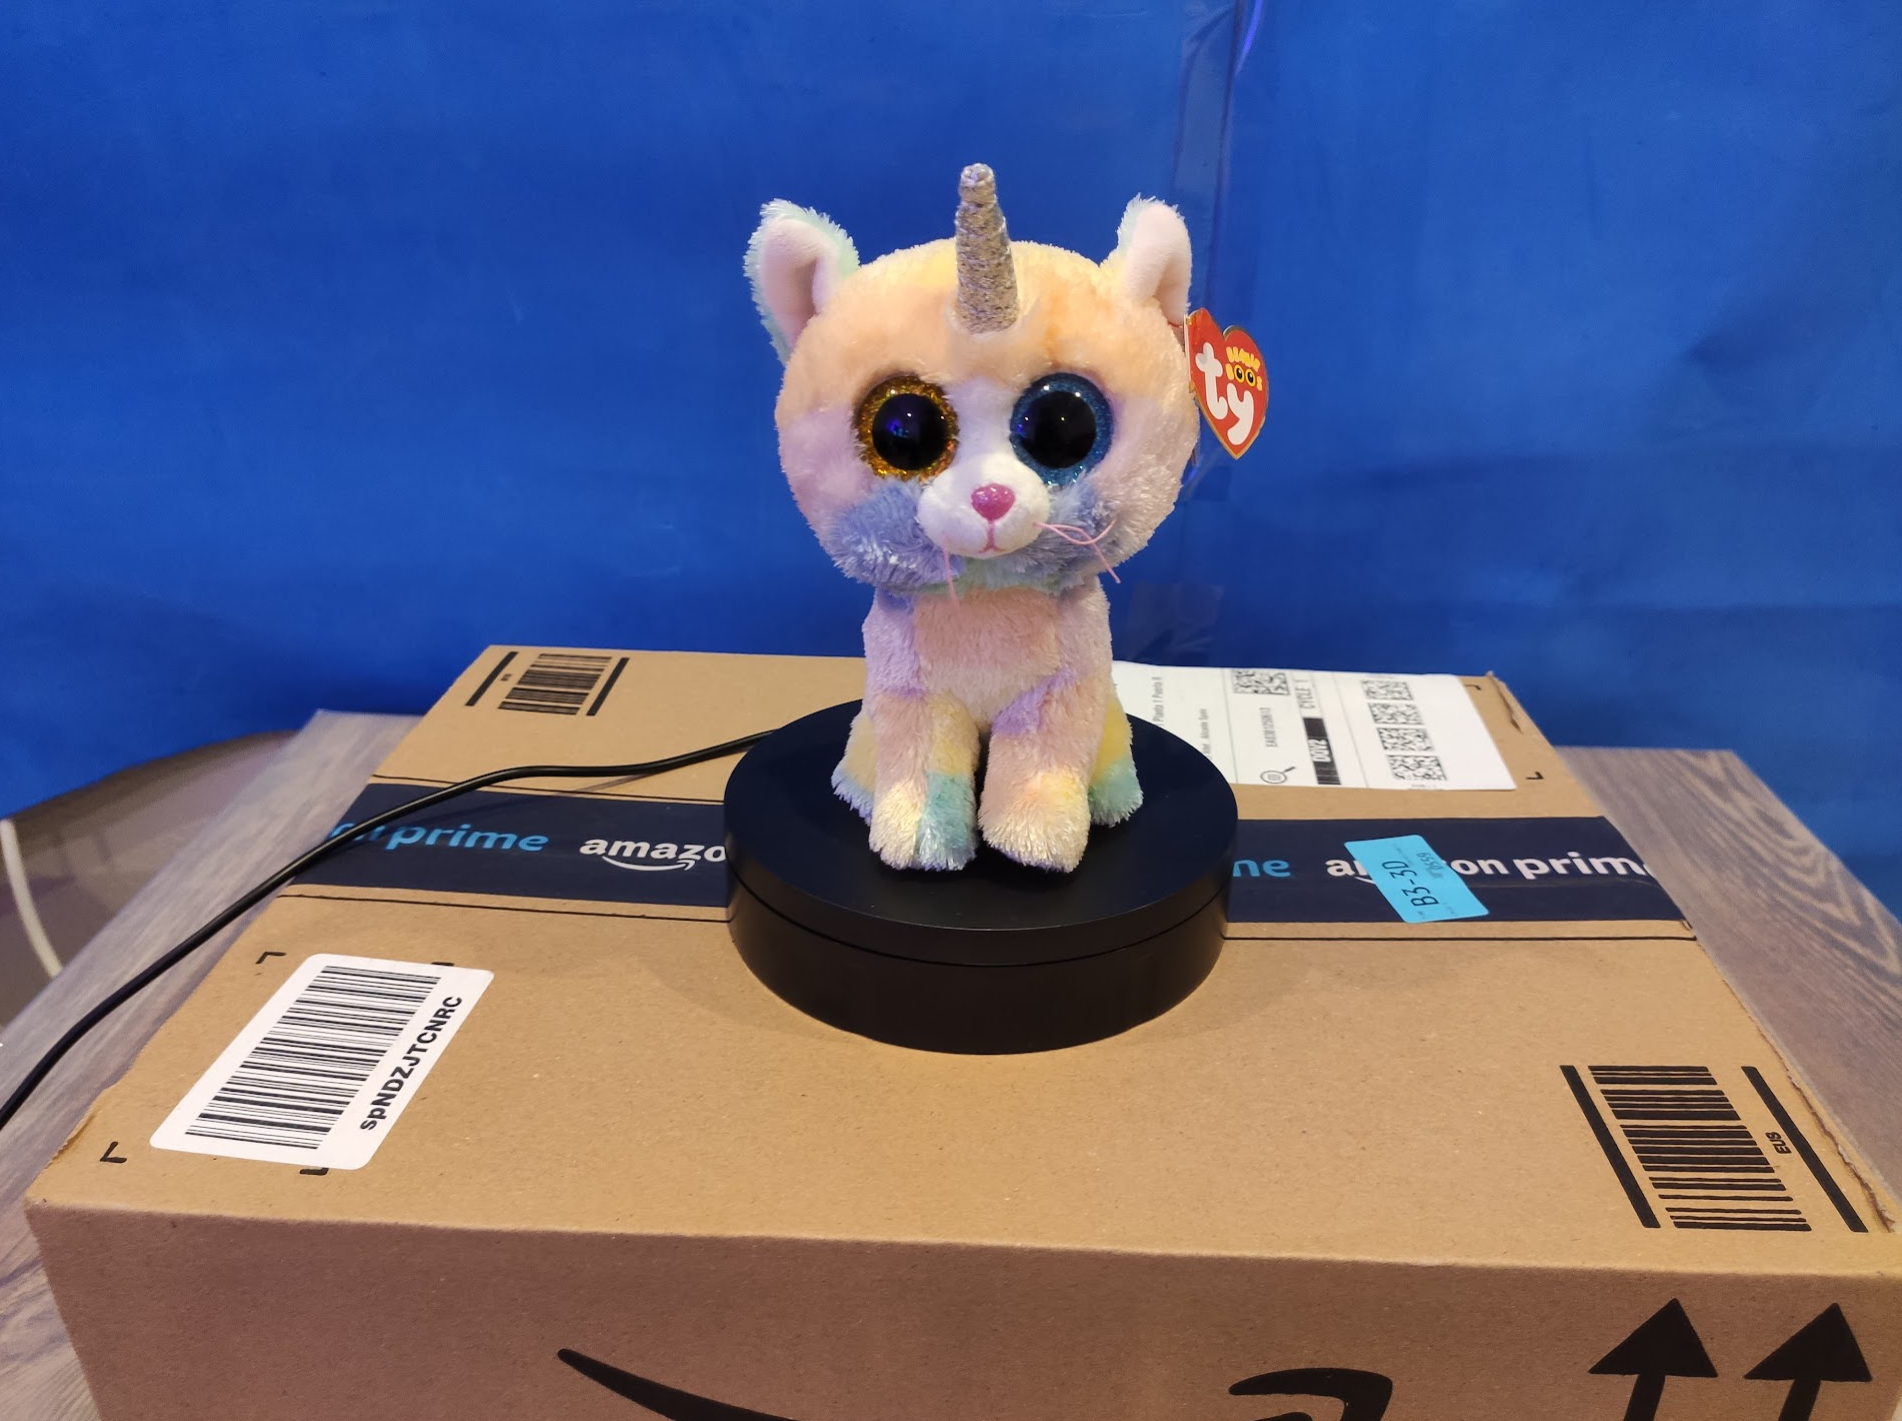
\includegraphics[height=3.5cm]{archivos/experimentacion-gato.png}
    \caption{Objeto de pruebas para reconstrucción 3D.}
    \label{fig:objetos-experimentacion}
\end{figure}

\section{Herramientas para visualizar las nubes de puntos}

Intel RealSense Viewer es una herramienta oficial de Intel para los sensores RealSense.
Con esta aplicación se puede visualizar la adquisición de la cámara en tiempo real, como se puede ver en la Figura \ref{fig:realsense-viewer-ejemplo}.
Tiene muchas herramientas y configuraciones que pueden ser útiles para experimentar con la cámara.

\begin{figure}[h]
    \centering
    \includegraphics[height=7cm]{archivos/intel-realsense-viewer.png}
    \caption{Captura de pantalla de Intel RealSense Viewer.}
    \label{fig:realsense-viewer-ejemplo}
\end{figure}

Otra herramienta interesante es MeshLab. Meshlab un software de código abierto para el procesamiento y edición de mallas triangulares no estructuradas en 3D \citep{RCDCS13} \citep{LocalChapterEvents:ItalChap:ItalianChapConf2008:129-136}.
Este sistema tiene varias herramientas para la edición, optimización, inspección y renderización de mallas.
Ha sido muy útil debido a la comodidad y facilidad con la que representa los datos en pantalla.
En la Figura \ref{fig:meshlab-ejemplo} podemos ver un ejemplo con tres nubes de puntos.
Fácilmente podemos diferenciar cada nube de puntos otorgándoles un color distinto y solapándolos.
Además, MeshLab contiene herramientas interesantes para el análisis de los resultados, pudiendo convertir las nubes de puntos resultantes en mallas \gls{3d} con mejor visualización \citep{kazhdan2013screened}.

\begin{figure}[h]
    \centering
    \includegraphics[height=7cm]{archivos/meshlab.png}
    \caption{Captura de pantalla de MeshLab con 3 nubes de puntos.}
    \label{fig:meshlab-ejemplo}
\end{figure}

\section{Resultados entre un modelo y una escena}

Para probar la solución del algoritmo \gls{icp} entre un modelo y una escena, utilizaremos un objeto rígido que rote ligeramente entre una captura y otra.
Para ello, utilizaremos las capturas de la Figura \ref{fig:objetos-experimentacion-modelo-escena}.

\begin{figure}[h]
    \centering
    \begin{subfigure}[t]{0.33\textheight}
    	\centering
        \includegraphics[height=3.5cm]{archivos/experimentacion-modelo.png}
        \caption{Modelo.}
    \end{subfigure}
    \begin{subfigure}[t]{0.33\textheight}
    	\centering
        \includegraphics[height=3.5cm]{archivos/experimentacion-escena.png}
        \caption{Escena.}
    \end{subfigure}
    \caption{Ejemplo de alineación de una escena con un modelo.}
    \label{fig:objetos-experimentacion-modelo-escena}
\end{figure}

En la Figura \ref{fig:experimentacion-1} podemos ver los resultado de aplicar los algoritmo \gls{icp} de \gls{pcl}, CUDA-ICP y \gls{cpd}.
Para lograr estos resultados se ha establecido un máximo de 200 iteraciones en los algoritmos, y un límite de distancia máxima de correspondencias de 0.01m, ya que las correpondencias deben ser muy cercanas.
Como se puede observar en las subfiguras \ref{fig:experimentacion-1-alineado-icp} y \ref{fig:experimentacion-1-alineado-cuda} la convergencia ha funcionado bastante bien y ambos resultados son muy parecidos.
Se ha probado a utilizar el algoritmo \gls{cpd} con la funcionalidad no rígida, sin embargo los resultados no son tan satisfactorios como se puede ver en la subfigura \ref{fig:experimentacion-1-alineado-cpd}.
Además, cabe mencionar que los tiempos para lograr estos resultados han sido de 0.97s para \gls{icp}, 0.72s para CUDA-ICP y 87.3s para \gls{cpd}.
Por el coste computacional tan elevado y los resultado obtenidos tras diversas pruebas con \gls{cpd} se ha decidido abandonar la idea de una transformación no rígida para centrarnos en los buenos resultados que nos pueden llegar a dar \gls{icp} y CUDA-ICP.

\begin{figure}[h]
    \centering
    \begin{subfigure}[t]{0.33\textheight}
    	\centering
        \includegraphics[height=5.5cm]{archivos/experimentacion-1-modelo.png}
        \caption{Nube de puntos modelo.}
    \end{subfigure}
    \begin{subfigure}[t]{0.33\textheight}
    	\centering
        \includegraphics[height=5.5cm]{archivos/experimentacion-1-escena.png}
        \caption{Nube de puntos escena.}
    \end{subfigure}
    \begin{subfigure}[t]{0.33\textheight}
    	\centering
        \includegraphics[height=5.5cm]{archivos/experimentacion-1-modelo-escena.png}
        \caption{Modelo y escena sin alinear.}
    \end{subfigure}
    \begin{subfigure}[t]{0.33\textheight}
    	\centering
        \includegraphics[height=5.5cm]{archivos/experimentacion-1-alineado-icp.png}
        \caption{Alineamiento con ICP.}
        \label{fig:experimentacion-1-alineado-icp}
    \end{subfigure}
    \begin{subfigure}[t]{0.33\textheight}
    	\centering
        \includegraphics[height=5.5cm]{archivos/experimentacion-1-alineado-cuda.png}
        \caption{Alineamiento con CUDA-ICP.}
        \label{fig:experimentacion-1-alineado-cuda}
    \end{subfigure}
    \begin{subfigure}[t]{0.33\textheight}
    	\centering
        \includegraphics[height=5.5cm]{archivos/experimentacion-1-alineado-cpd.png}
        \caption{Alineamiento con CPD.}
        \label{fig:experimentacion-1-alineado-cpd}
    \end{subfigure}
    \caption{Resultados experimentación modelo y escena alineados.}
    \label{fig:experimentacion-1}
\end{figure}

\section{Resultados de la reconstrucción completa con un objeto}

Para la reconstrucción completa de un modelo \gls{3d} comenzaremos experimentando con el objeto de pruebas de la Figura \ref{fig:objetos-experimentacion} y, finalmente, se realizarán pruebas con el cuerpo humano.
En estas pruebas se utilizarán los algoritmos \gls{icp} y CUDA-ICP para comparar la calidad de la reconstrucción y los tiempos empleados en el dispositivo Jetson Nano.
Comenzaremos con el objeto de pruebas que ya hemos utilizado anteriormente.

Tras la fase de adquisición y pre-procesamiento obtenemos las capturas desde distintos ángulos del objeto.
El objeto ha estado girando con velocidad constante en un plato giratorio que tarda 21 segundos en realizar una vuelta 360º y para la fase de adquisición se ha establecido que el sensor capture imágenes cada 0.5 segundos.
Por tanto, obtenemos un total de 42 capturas del objeto.
A continuación, la primera de estas capturas será interpretada como el modelo y el resto irán siendo alineadas consecutivamente, hasta tener la reconstrucción completa.

En las Figuras \ref{fig:resultados-reconstruccion-objeto-icp} y \ref{fig:resultados-reconstruccion-objeto-cuda} podemos ver los resultados de las reconstrucción con \gls{icp} y CUDA-ICP, respectivamente.
Las cuatro primeras imágenes muestran el resultado de la nube de puntos reconstruida completamente, las siguientes cuatro imágenes muestran la reconstrucción de una malla generada a partir de la nube de puntos.

En la Tabla \ref{tab:resultado-objeto} tenemos datos interesantes respecto a los tiempos de reconstrucción. En la primer columna se indica el número de iteración que está pasando, seguidamente se indica la cantidad de puntos que tenía la escena en esa iteración, a continuación se expresa el tiempo que ha tardado la iteración en alinearse utilizando \gls{icp} y el tiempo total acumulado, seguidamente los mismos tiempos para CUDA-ICP, y finalmente los porcentajes de mejora de velocidad usando CUDA-ICP frente a \gls{icp} respecto al tiempo que tarda la iteración en sí y respecto al tiempo total.

Tras analizar los resultados vemos que los tiempos de ejecución de CUDA-ICP son mucho más rápidos que el algoritmo \gls{icp}, por lo que hay una buena mejora al estar aprovechando los núcleos de la gráfica, sin embargo el resultado final no ha conseguido converger tan bien como lo ha hecho \gls{icp} en \gls{pcl}.

\begin{figure}[h]
    \centering
    \begin{subfigure}[t]{0.2\textheight}
    	\centering
        \includegraphics[height=4.5cm]{archivos/experimentacion-2-resultado-nube.png}
    \end{subfigure}
    \begin{subfigure}[t]{0.2\textheight}
    	\centering
        \includegraphics[height=4.5cm]{archivos/experimentacion-2-resultado-nube-2.png}
    \end{subfigure}
    \begin{subfigure}[t]{0.2\textheight}
    	\centering
        \includegraphics[height=4.5cm]{archivos/experimentacion-2-resultado-nube-3.png}
    \end{subfigure}
    \begin{subfigure}[t]{0.2\textheight}
    	\centering
        \includegraphics[height=4.5cm]{archivos/experimentacion-2-resultado-nube-4.png}
    \end{subfigure}
    \begin{subfigure}[t]{0.2\textheight}
    	\centering
        \includegraphics[height=4.5cm]{archivos/experimentacion-2-resultado-malla.png}
    \end{subfigure}
    \begin{subfigure}[t]{0.2\textheight}
    	\centering
        \includegraphics[height=4.5cm]{archivos/experimentacion-2-resultado-malla-2.png}
    \end{subfigure}
    \begin{subfigure}[t]{0.2\textheight}
    	\centering
        \includegraphics[height=4.5cm]{archivos/experimentacion-2-resultado-malla-3.png}
    \end{subfigure}
    \begin{subfigure}[t]{0.2\textheight}
    	\centering
        \includegraphics[height=4.5cm]{archivos/experimentacion-2-resultado-malla-4.png}
    \end{subfigure}
    \caption{Resultados de Reconstrucción 3D con objeto usando ICP.}
    \label{fig:resultados-reconstruccion-objeto-icp}
\end{figure}

\begin{figure}[h]
    \centering
    \begin{subfigure}[t]{0.2\textheight}
    	\centering
        \includegraphics[height=4.5cm]{archivos/experimentacion-3-resultado-nube.png}
    \end{subfigure}
    \begin{subfigure}[t]{0.2\textheight}
    	\centering
        \includegraphics[height=4.5cm]{archivos/experimentacion-3-resultado-nube-2.png}
    \end{subfigure}
    \begin{subfigure}[t]{0.2\textheight}
    	\centering
        \includegraphics[height=4.5cm]{archivos/experimentacion-3-resultado-nube-3.png}
    \end{subfigure}
    \begin{subfigure}[t]{0.2\textheight}
    	\centering
        \includegraphics[height=4.5cm]{archivos/experimentacion-3-resultado-nube-4.png}
    \end{subfigure}
    \begin{subfigure}[t]{0.2\textheight}
    	\centering
        \includegraphics[height=4.5cm]{archivos/experimentacion-3-resultado-malla.png}
    \end{subfigure}
    \begin{subfigure}[t]{0.2\textheight}
    	\centering
        \includegraphics[height=4.5cm]{archivos/experimentacion-3-resultado-malla-2.png}
    \end{subfigure}
    \begin{subfigure}[t]{0.2\textheight}
    	\centering
        \includegraphics[height=4.5cm]{archivos/experimentacion-3-resultado-malla-3.png}
    \end{subfigure}
    \begin{subfigure}[t]{0.2\textheight}
    	\centering
        \includegraphics[height=4.5cm]{archivos/experimentacion-3-resultado-malla-4.png}
    \end{subfigure}
    \caption{Resultados de Reconstrucción 3D con objeto usando CUDA-ICP.}
    \label{fig:resultados-reconstruccion-objeto-cuda}
\end{figure}

\begin{table}[h]
    \centering
      \begin{tabular}{rrrrrrrr}
            &       & \multicolumn{2}{c}{Tiempo ICP (s)} & \multicolumn{2}{c}{Tiempo CUDA-ICP (s)} & \multicolumn{2}{c}{Mejora de velocidad} \\
      \multicolumn{1}{l}{Iteración} & \multicolumn{1}{l}{Puntos} & \multicolumn{1}{l}{t/iteracion} & \multicolumn{1}{l}{Total} & \multicolumn{1}{l}{t/iteracion} & \multicolumn{1}{l}{Total} & \multicolumn{1}{l}{\%/iteración} & \multicolumn{1}{l}{Total} \\
      0     & 3540  &       &       &       &       &       &  \\
      1     & 3523  & 1,837 & 1,837 & 0,607 & 0,607 & 302,37\% & 302,37\% \\
      2     & 3497  & 3,056 & 4,892 & 0,977 & 1,585 & 312,62\% & 308,69\% \\
      3     & 3557  & 4,613 & 9,505 & 1,121 & 2,705 & 411,64\% & 351,33\% \\
      4     & 3597  & 3,982 & 13,487 & 0,984 & 3,689 & 404,79\% & 365,59\% \\
      5     & 3710  & 4,133 & 17,620 & 1,159 & 4,849 & 356,47\% & 363,41\% \\
      6     & 3702  & 5,726 & 23,346 & 1,125 & 5,973 & 509,01\% & 390,83\% \\
      7     & 3634  & 3,965 & 27,311 & 1,035 & 7,009 & 382,93\% & 389,66\% \\
      8     & 3755  & 3,877 & 31,188 & 1,051 & 8,060 & 368,94\% & 386,96\% \\
      9     & 3686  & 4,259 & 35,446 & 1,305 & 9,365 & 326,30\% & 378,50\% \\
      10    & 3792  & 3,364 & 38,811 & 1,012 & 10,377 & 332,35\% & 374,00\% \\
      11    & 3775  & 3,536 & 42,347 & 1,315 & 11,693 & 268,81\% & 362,17\% \\
      12    & 3883  & 3,586 & 45,933 & 0,971 & 12,663 & 369,47\% & 362,73\% \\
      13    & 3855  & 3,746 & 49,678 & 1,163 & 13,827 & 321,95\% & 359,30\% \\
      14    & 3842  & 7,131 & 56,809 & 1,375 & 15,201 & 518,65\% & 373,71\% \\
      15    & 3994  & 5,695 & 62,504 & 1,217 & 16,419 & 467,87\% & 380,69\% \\
      16    & 4127  & 6,641 & 69,145 & 1,292 & 17,711 & 514,04\% & 390,42\% \\
      17    & 4443  & 6,107 & 75,252 & 1,198 & 18,909 & 509,77\% & 397,98\% \\
      18    & 4268  & 4,798 & 80,050 & 1,621 & 20,530 & 295,94\% & 389,92\% \\
      19    & 4128  & 5,402 & 85,451 & 1,464 & 21,993 & 369,04\% & 388,53\% \\
      20    & 3955  & 5,822 & 91,273 & 1,315 & 23,309 & 442,66\% & 391,59\% \\
      21    & 3931  & 4,329 & 95,602 & 1,262 & 24,570 & 343,10\% & 389,10\% \\
      22    & 4000  & 5,393 & 100,995 & 1,587 & 26,157 & 339,94\% & 386,11\% \\
      23    & 3922  & 6,951 & 107,947 & 1,553 & 27,710 & 447,57\% & 389,56\% \\
      24    & 3828  & 5,326 & 113,272 & 1,621 & 29,331 & 328,51\% & 386,18\% \\
      25    & 3739  & 6,527 & 119,799 & 1,574 & 30,905 & 414,58\% & 387,63\% \\
      26    & 3687  & 5,665 & 125,464 & 1,531 & 32,436 & 370,08\% & 386,80\% \\
      27    & 3665  & 7,183 & 132,647 & 1,810 & 34,246 & 396,91\% & 387,34\% \\
      28    & 3658  & 8,995 & 141,642 & 1,468 & 35,714 & 612,74\% & 396,60\% \\
      29    & 3746  & 6,553 & 148,195 & 1,497 & 37,211 & 437,62\% & 398,25\% \\
      30    & 3747  & 8,390 & 156,585 & 1,774 & 38,985 & 473,00\% & 401,65\% \\
      31    & 3632  & 9,176 & 165,761 & 1,908 & 40,893 & 480,98\% & 405,35\% \\
      32    & 3516  & 8,287 & 174,048 & 1,726 & 42,619 & 480,13\% & 408,38\% \\
      33    & 3497  & 5,666 & 179,714 & 1,971 & 44,590 & 287,51\% & 403,04\% \\
      34    & 3513  & 5,748 & 185,462 & 1,948 & 46,538 & 295,03\% & 398,52\% \\
      35    & 3522  & 5,483 & 190,945 & 1,837 & 48,375 & 298,48\% & 394,72\% \\
      36    & 3558  & 5,042 & 195,986 & 1,798 & 50,173 & 280,45\% & 390,62\% \\
      37    & 3613  & 5,722 & 201,708 & 1,961 & 52,134 & 291,73\% & 386,90\% \\
      38    & 3678  & 5,355 & 207,063 & 1,835 & 53,969 & 291,74\% & 383,67\% \\
      39    & 3693  & 8,961 & 216,024 & 1,999 & 55,969 & 448,18\% & 385,97\% \\
      40    & 3638  & 6,771 & 222,795 & 1,999 & 57,967 & 338,78\% & 384,34\% \\
      41    & 3662  & 8,201 & 230,996 & 1,928 & 59,896 & 425,32\% & 385,66\% \\
    \end{tabular}%
    \caption{Resultados de Reconstrucción 3D con objeto.}
    \label{tab:resultado-objeto}%
\end{table}%
  

\section{Resultados de la reconstrucción completa de un cuerpo humano}

Para lograr un buen resultado en la reconstrucción del cuerpo humano se ha realizado la fase de adquisición con el sujeto sentado en una silla de oficina, de esta forma el sujeto puede rotar cómodamente 360º intentando mantener su cuerpo rígido de forma que la reconstrucción sea más limpia.
En esta fase de adquisición se han realizado 30 capturas al sujeto, que es lo que ha tardado en rotar 360º con una frecuencia de capturación de 1 imágen por cada 0.5 segundos.

Para el algoritmo \gls{icp} se ha establecido un máximo de 200 iteraciones y el límite máximo de distancia entre correspondencias se ha subido a 0.5m debido a que el cuerpo a escanear es mucho más grande y se mueve a una velocidad que no es constante como sí lo hacía el objeto encima del plato giratorio, por lo que es posible que alguna distancia pueda llegar a medir más.

De nuevo, en las figuras \ref{fig:resultados-reconstruccion-cuerpo-icp} y \ref{fig:resultados-reconstruccion-cuerpo-cuda} podemos ver los resultados de la reconstrucción expresados de la misma forma que el objeto, es decir, las primeras cuatro imágenes en nubes de puntos, y las siguientes cuatro con una malla generada a partir de los puntos.

Si analizamos la Tabla \ref{tab:resultado-cuerpo}, podemos ver que los resultados son parecido al del objeto, con unos tiempos en general más grandes debido a que la cantidad de puntos de cada escena es mucho mayor comparado con las escenas del objeto.
Aunque el algoritmo con \gls{cuda} vuelve a ser mucho más rápido, volvemos a tener el problema de que el resultado no es tan correcto como lo es en \gls{icp} de \gls{pcl}.
Este es un problema que tenemos con la librería de \gls{cuda} ya que no permite mucha configuración a la hora de lanzar el algoritmo, como si lo hace \gls{pcl}, y no se ha podido corregir el error.

\begin{figure}[h]
    \centering
    \begin{subfigure}[t]{0.2\textheight}
    	\centering
        \includegraphics[height=4.5cm]{archivos/experimentacion-4-resultado-nube.png}
    \end{subfigure}
    \begin{subfigure}[t]{0.2\textheight}
    	\centering
        \includegraphics[height=4.5cm]{archivos/experimentacion-4-resultado-nube-2.png}
    \end{subfigure}
    \begin{subfigure}[t]{0.2\textheight}
    	\centering
        \includegraphics[height=4.5cm]{archivos/experimentacion-4-resultado-nube-3.png}
    \end{subfigure}
    \begin{subfigure}[t]{0.2\textheight}
    	\centering
        \includegraphics[height=4.5cm]{archivos/experimentacion-4-resultado-nube-4.png}
    \end{subfigure}
    \begin{subfigure}[t]{0.2\textheight}
    	\centering
        \includegraphics[height=4.5cm]{archivos/experimentacion-4-resultado-nube-5.png}
    \end{subfigure}
    \begin{subfigure}[t]{0.2\textheight}
    	\centering
        \includegraphics[height=4.5cm]{archivos/experimentacion-4-resultado-malla.png}
    \end{subfigure}
    \begin{subfigure}[t]{0.2\textheight}
    	\centering
        \includegraphics[height=4.5cm]{archivos/experimentacion-4-resultado-malla-2.png}
    \end{subfigure}
    \begin{subfigure}[t]{0.2\textheight}
    	\centering
        \includegraphics[height=4.5cm]{archivos/experimentacion-4-resultado-malla-3.png}
    \end{subfigure}
    \begin{subfigure}[t]{0.2\textheight}
    	\centering
        \includegraphics[height=4.5cm]{archivos/experimentacion-4-resultado-malla-4.png}
    \end{subfigure}
    \begin{subfigure}[t]{0.2\textheight}
    	\centering
        \includegraphics[height=4.5cm]{archivos/experimentacion-4-resultado-malla-5.png}
    \end{subfigure}
    \caption{Resultados de Reconstrucción 3D de un cuerpo humano usando ICP.}
    \label{fig:resultados-reconstruccion-cuerpo-icp}
\end{figure}

\begin{figure}[h]
    \centering
    \begin{subfigure}[t]{0.2\textheight}
    	\centering
        \includegraphics[height=4.5cm]{archivos/experimentacion-5-resultado-nube.png}
    \end{subfigure}
    \begin{subfigure}[t]{0.2\textheight}
    	\centering
        \includegraphics[height=4.5cm]{archivos/experimentacion-5-resultado-nube-2.png}
    \end{subfigure}
    \begin{subfigure}[t]{0.2\textheight}
    	\centering
        \includegraphics[height=4.5cm]{archivos/experimentacion-5-resultado-nube-3.png}
    \end{subfigure}
    \begin{subfigure}[t]{0.2\textheight}
    	\centering
        \includegraphics[height=4.5cm]{archivos/experimentacion-5-resultado-nube-4.png}
    \end{subfigure}
    \begin{subfigure}[t]{0.2\textheight}
    	\centering
        \includegraphics[height=4.5cm]{archivos/experimentacion-5-resultado-nube-5.png}
    \end{subfigure}
    \begin{subfigure}[t]{0.2\textheight}
    	\centering
        \includegraphics[height=4.5cm]{archivos/experimentacion-5-resultado-malla.png}
    \end{subfigure}
    \begin{subfigure}[t]{0.2\textheight}
    	\centering
        \includegraphics[height=4.5cm]{archivos/experimentacion-5-resultado-malla-2.png}
    \end{subfigure}
    \begin{subfigure}[t]{0.2\textheight}
    	\centering
        \includegraphics[height=4.5cm]{archivos/experimentacion-5-resultado-malla-3.png}
    \end{subfigure}
    \begin{subfigure}[t]{0.2\textheight}
    	\centering
        \includegraphics[height=4.5cm]{archivos/experimentacion-5-resultado-malla-4.png}
    \end{subfigure}
    \begin{subfigure}[t]{0.2\textheight}
    	\centering
        \includegraphics[height=4.5cm]{archivos/experimentacion-5-resultado-malla-5.png}
    \end{subfigure}
    \caption{Resultados de Reconstrucción 3D de un cuerpo humano usando CUDA-ICP.}
    \label{fig:resultados-reconstruccion-cuerpo-cuda}
\end{figure}

\begin{table}[h]
    \centering
      \begin{tabular}{rrrrrrrr}
            &       & \multicolumn{2}{c}{Tiempo ICP (s)} & \multicolumn{2}{c}{Tiempo CUDA-ICP (s)} & \multicolumn{2}{c}{Mejora de velocidad} \\
      \multicolumn{1}{l}{Iteración} & \multicolumn{1}{l}{Puntos} & \multicolumn{1}{l}{t/iteracion} & \multicolumn{1}{l}{Total} & \multicolumn{1}{l}{t/iteracion} & \multicolumn{1}{l}{Total} & \multicolumn{1}{l}{\%/iteración} & \multicolumn{1}{l}{Total} \\
      0     & 19256 &       &       &       &       &       &  \\
      1     & 19164 & 11,020 & 11,020 & 3,189 & 3,189 & 345,56\% & 345,56\% \\
      2     & 19021 & 18,334 & 29,354 & 5,132 & 8,321 & 357,28\% & 352,79\% \\
      3     & 19349 & 27,676 & 57,030 & 5,883 & 14,204 & 470,44\% & 401,52\% \\
      4     & 19569 & 23,892 & 80,922 & 5,165 & 19,368 & 462,62\% & 417,81\% \\
      5     & 20181 & 24,798 & 105,720 & 6,087 & 25,455 & 407,39\% & 415,32\% \\
      6     & 20137 & 34,354 & 140,074 & 5,906 & 31,361 & 581,73\% & 446,66\% \\
      7     & 19768 & 23,790 & 163,864 & 5,436 & 36,797 & 437,64\% & 445,32\% \\
      8     & 20426 & 23,262 & 187,126 & 5,517 & 42,314 & 421,64\% & 442,24\% \\
      9     & 20052 & 25,552 & 212,678 & 6,852 & 49,166 & 372,91\% & 432,58\% \\
      10    & 20626 & 20,186 & 232,864 & 5,315 & 54,480 & 379,83\% & 427,43\% \\
      11    & 20536 & 21,216 & 254,080 & 6,906 & 61,386 & 307,21\% & 413,91\% \\
      12    & 21124 & 21,516 & 275,596 & 5,096 & 66,482 & 422,25\% & 414,55\% \\
      13    & 20973 & 22,474 & 298,070 & 6,108 & 72,590 & 367,94\% & 410,62\% \\
      14    & 20902 & 42,784 & 340,854 & 7,218 & 79,808 & 592,74\% & 427,10\% \\
      15    & 21729 & 34,168 & 375,022 & 6,390 & 86,198 & 534,71\% & 435,07\% \\
      16    & 22452 & 39,848 & 414,870 & 6,783 & 92,981 & 587,47\% & 446,19\% \\
      17    & 24171 & 36,642 & 451,512 & 6,290 & 99,270 & 582,59\% & 454,83\% \\
      18    & 23220 & 28,786 & 480,298 & 8,511 & 107,781 & 338,22\% & 445,62\% \\
      19    & 22454 & 32,410 & 512,708 & 7,685 & 115,466 & 421,76\% & 444,04\% \\
      20    & 21515 & 34,930 & 547,638 & 6,904 & 122,370 & 505,90\% & 447,53\% \\
      21    & 21384 & 25,974 & 573,612 & 6,624 & 128,994 & 392,12\% & 444,68\% \\
      22    & 21760 & 32,360 & 605,972 & 8,330 & 137,324 & 388,50\% & 441,27\% \\
      23    & 21333 & 41,708 & 647,680 & 8,154 & 145,478 & 511,50\% & 445,21\% \\
      24    & 20827 & 31,954 & 679,634 & 8,511 & 153,989 & 375,44\% & 441,35\% \\
      25    & 20341 & 39,160 & 718,794 & 8,265 & 162,254 & 473,81\% & 443,01\% \\
      26    & 20055 & 33,992 & 752,786 & 8,037 & 170,291 & 422,94\% & 442,06\% \\
      27    & 19938 & 43,098 & 795,884 & 9,501 & 179,792 & 453,62\% & 442,67\% \\
      28    & 19902 & 53,970 & 849,854 & 7,707 & 187,499 & 700,27\% & 453,26\% \\
      29    & 20376 & 39,318 & 889,172 & 7,862 & 195,360 & 500,13\% & 455,15\% \\
      30    & 20385 & 50,338 & 939,510 & 9,312 & 204,672 & 540,57\% & 459,03\% \\
      31    & 19757 & 55,054 & 994,564 & 10,016 & 214,688 & 549,69\% & 463,26\% \\
    \end{tabular}%
    \caption{Resultados de Reconstrucción 3D de un cuerpo humano.}
    \label{tab:resultado-cuerpo}%
\end{table}%
  
\chapter{Conclusión}
\label{cap:conclusion}

En este trabajo se presenta un sistema económico y portable que es capaz de reconstruir objetos y cuerpos en \gls{3d} de forma eficiente utilizando un sensor \gls{rgbd} y un pequeño computador embebido que es capaz de aprovechar la \gls{gpu} para acelerar el funcionamiento.
Se ha implementado uno de los métodos de registro de nubes de puntos más utilizado haciendo uso de la librería \gls{pcl} y se ha conseguido usar aprovechando la concurrencia en el algoritmo con los núcleos de la \gls{gpu}.
Sin embargo, se ha hecho uso de una librería oficial implementada por Nvidia que no proporciona mucho margen para personalizarla, lo que ha sido un problema para obtener resultados de buena calidad.
Se plantea como mejora a corto plazo para este trabajo la posibilidad de desarrollar una implementación del algoritmo \gls{icp} personalizada, que de juego a modificar parámetros para conseguir mejores resultados.

Por otro lado, también es interesante como mejora a corto plazo seguir investigando en la línea de los métodos de registro no rígidos, desarrollando también una versión personalizada del algoritmo \gls{pcl} que utilice \gls{cuda} y pueda aprovechar los núcleos de la \gls{gpu}.
De esta forma podría llegar a ser viable la ejecución de estos algoritmos en este sistema, lo cual implicaría una mejora de calidad en las reconstrucciones sobre cuerpos humanos debido a que permitiría realizar una reconstrucción \gls{3d} con modelos no rígidos.

%%%%
% CONTENIDO. Anexos - Añade o elimina según tus necesidades
%%%%
% \appendix % Inicio de los apéndices
% \chapter{Entorno experimental}

Con el objetivo de realizar la reconstrucción de cuerpos u objetos en modelos \gls{3d} se ha creado un pequeño entorno experimental donde realizar las pruebas.
El entorno está compuesto por el sensor Intel RealSense D435, montado en un trípode y con posición fija y un plato giratorio para las pruebas con objetos pequeños y rígidos.

En la Figura \ref{fig:entorno-experimental} podemos ver un objeto encima del plato giratorio y el sensor Intel Realsense D435 montado en el trípode.

\begin{figure}[h]
    \centering
    \includegraphics[width=\textwidth]{archivos/entorno-experimental-2.jpg}
    \caption{Entorno experimental.}
    \label{fig:entorno-experimental}
\end{figure}

El plato sobre el que está subido el objeto es un plato con velocidad fija que rota indefinidamente.
Utilizarlo facilita la tarea de reconstrucción \gls{3d} sobre los objetos ya que con el plato no necesitan ninguna interacción extra para rotar y ser capturados por todos los ángulos.
Esto ha facilitado la tarea de experimentación en objetos rígidos para su posterior prueba en cuerpos humanos.

La pared está cubierta con un panel de poliestireno azul con la finalidad de reducir ruido en la adquisición de datos, debido a que el sensor tiene pequeños fallos a la hora de identificar zonas concretas y muy detalladas y se llega a equivocar en el cálculo de profundidad de algunas zonas.
No obstante, aunque el poliestireno ha ayudado un poco, tampoco ha marcado gran diferencia, ya que esto ha seguido ocurriendo.

% \begin{figure}[h]
%     \centering
%     \begin{subfigure}[h]{0.5\textheight}
%     	\centering
%         \includegraphics[width=\textwidth]{archivos/entorno-experimental-2.jpg}
%     \end{subfigure}
%     \begin{subfigure}[h]{0.6\textheight}
%     	\centering
%         \includegraphics[width=\textwidth, angle=270]{archivos/entorno-experimental-1.jpg}
%     \end{subfigure}
%     \caption{Entorno experimental.}
%     \label{fig:entorno-experimental}
% \end{figure}
\appendix
\chapter*{Anexos}% If \appendix doesn't insert a \chapter
\addcontentsline{toc}{chapter}{Anexos}% Print Appendix in ToC
\setcounter{section}{0}% Reset numbering for sections
\renewcommand{\thesection}{\Alph{section}}% Adjust section printing (from here onward)
\chapter{Entorno experimental}

Con el objetivo de realizar la reconstrucción de cuerpos u objetos en modelos \gls{3d} se ha creado un pequeño entorno experimental donde realizar las pruebas.
El entorno está compuesto por el sensor Intel RealSense D435, montado en un trípode y con posición fija y un plato giratorio para las pruebas con objetos pequeños y rígidos.

En la Figura \ref{fig:entorno-experimental} podemos ver un objeto encima del plato giratorio y el sensor Intel Realsense D435 montado en el trípode.

\begin{figure}[h]
    \centering
    \includegraphics[width=\textwidth]{archivos/entorno-experimental-2.jpg}
    \caption{Entorno experimental.}
    \label{fig:entorno-experimental}
\end{figure}

El plato sobre el que está subido el objeto es un plato con velocidad fija que rota indefinidamente.
Utilizarlo facilita la tarea de reconstrucción \gls{3d} sobre los objetos ya que con el plato no necesitan ninguna interacción extra para rotar y ser capturados por todos los ángulos.
Esto ha facilitado la tarea de experimentación en objetos rígidos para su posterior prueba en cuerpos humanos.

La pared está cubierta con un panel de poliestireno azul con la finalidad de reducir ruido en la adquisición de datos, debido a que el sensor tiene pequeños fallos a la hora de identificar zonas concretas y muy detalladas y se llega a equivocar en el cálculo de profundidad de algunas zonas.
No obstante, aunque el poliestireno ha ayudado un poco, tampoco ha marcado gran diferencia, ya que esto ha seguido ocurriendo.

% \begin{figure}[h]
%     \centering
%     \begin{subfigure}[h]{0.5\textheight}
%     	\centering
%         \includegraphics[width=\textwidth]{archivos/entorno-experimental-2.jpg}
%     \end{subfigure}
%     \begin{subfigure}[h]{0.6\textheight}
%     	\centering
%         \includegraphics[width=\textwidth, angle=270]{archivos/entorno-experimental-1.jpg}
%     \end{subfigure}
%     \caption{Entorno experimental.}
%     \label{fig:entorno-experimental}
% \end{figure}
% \chapter{Calibración de los sensores.}

\todo[inline]{Enseñar los errores que pueden dar las capturas y explicar que es un problema de calibración y como se podría mejorar.}

% Por otro lado, buscando investigaciones relacionadas con el sensor, en ``Análisis comparativo de métodos de calibrado para sensores RGB-D y su influencia en el registro de múltiples vistas'' de \citep{VillenaMartinez2015} se demuestra que los parámetros por defecto que se utilizan en los sensores \gls{rgbd} pueden no ser lo suficientemente precisos.
% Por tanto es necesario hacer un estudio previo de métodos de calibrado para la obtención de mejores resultados.
% El calibrado en sensores \gls{rgbd} consiste en encontrar los parámetros adecuados para el sensor permitiendo mejorar la exactitud de los datos obtenidos.
% Estos datos consistirán en la información del color y la profundidad en la escena.

% Existen dos tipos de calibrados:
% intrínseco y extrínseco.

% \begin{description}
%     \item[Calibrado intrínseco:]
    
%     es aquel que se centra en los parámetros internos del sensor.

%     Uno de esos parámetros es la distancia entre el centro óptico y el plano focal donde se proyecta la imagen, conocida como distancia o longitud focal.
%     Ésta permite estimar el campo de visión de la cámara.

%     Otro parámetro es el punto principal que representa el desplazamiento del eje óptico respecto al sensor, provocando un desplazamiento en la proyección de la imagen.

%     Las distorsiones ópticas debido a fallos en el diseño o fabricación de las lentes es otro parámetro a tener en cuenta.
%     Esta distorsión puede ser una distorsión radial (lentes que no son perfectamente parabólicas) o tangencial (lente que no es paralela totalmente con el sensor).

%     \item[Calibrado extrínseco:]
    
%     se refiere al tipo de calibrado que se centra en las características externas.
%     Un ejemplo de ello sería el alineamiento de una cámara estereoscópica.

%     Consiste en el proceso de situar las imágenes obtenidas por ambos sensores del mismo sistema.
%     Para ello es necesario conocer las matrices de rotación y traslación que permitan aplicar la transformación necesaria para que las imágenes obtenidas queden situadas en un eje de coordenadas común.
% \end{description}

% En ``A Quantitative Comparison of Calibration Methods for RGB-D Sensors Using Different Technologies'', trabajo de investigación de \citep{VillenaMartinez2017} se trató de analizar tres métodos distintos de calibración con la finalidad de encontrar el mejor método de calibrado para mejorar la exactitud de los datos obtenidos.
% Se comparan los métodos de Bouguet, Burrus y Herrera.

% El método de \citep{bouguet2004camera} intenta calibrar la cámara RGB y el sensor de profundidad como si se tratase de un sistema estéreo, aplicando transformaciones para obtener las correspondencias entre el mapa de profundidad y la imagen de color.

% El método de \citep{burrus2012rgbdemo} también realiza el proceso de calibración como si se tratase de un sistema estéreo.
% A partir de la información del patrón en ambas cámaras se realiza una calibración para obtener los parámetros extrínsecos que permiten alinear las imágenes de ambas c    ámaras (color y profundidad).

% El método de \citep{HerreraC.2012} permite calibrar simultáneamente la posición relativa entre dos cámaras de color y una cámara de profundidad.
% Además, ha sido diseñado con el objetivo de ser aplicable a varios sensores.

% De todas las pruebas realizadas en dicha investigación, el método de Herrera es el que mejores resultados obtiene generalmente.

% También merece la pena tener en cuenta un algoritmo llamado \gls{mclse}.
% En el artículo científico ``Iterative multilinear optimization for planar model fitting under geometric constraints'' de \citep{Azorin-Lopez2021} presentan este algoritmo como un método de calibrado extrínseco para el cálculo de modelos planares con restricciones.
% Se trata de un algoritmo muy rápido y preciso.
\chapter{Estructura del proyecto subido a GitHub}

El código fuente de todo el proyecto está subido en un repositorio público en GitHub y es accesible para poder realizar las mismas pruebas desarrolladas en este \gls{tfg}.

El proyecto entero se puede encontrar en \href{https://github.com/ems107/EdgarMartinezSerranoTFG}{GitHub} desde el siguiente enlace:

\href{https://github.com/ems107/EdgarMartinezSerranoTFG}{https://github.com/ems107/EdgarMartinezSerranoTFG}.

Dentro de la estructura del proyecto, nos encontraremos con un README que nos explicará cómo compilar y ejecutar del proyecto.

\begin{figure}[h]
    \centering
    \includegraphics[height=6cm]{archivos/estructura-proyecto.png}
    \caption{Estructura del proyecto en GitHub.}
    \label{fig:estructura-proyecto}
\end{figure}

En la Figura \ref{fig:estructura-proyecto} podemos ver cómo se estructura el repositorio.
Por un lado tenemos el directorio ``Latex'' donde podemos encontrar todo el código fuente utilizado para construir esta memoria, y la memoria en sí.

Por otro lado, dentro del directorio ``Code Solutions'' encontraremos todo el código utilizado en el \gls{tfg}.
Dentro del subdirectorio ``JetsonNano'' encontramos el proyecto CMake que se ha estado explicando detalladamente en la memoria.
En el subdirectorio ``JetsonNanoWindowsTesting'' encontramos una solución en Visual Studio capaz de ejecutar el mismo código que ha sido desarrollado en la Jetson para testear en Windows, excluyendo la librería de CUDA-ICP que no funciona en Windows.
Por último, los subdirectorios ``PointCloudLibraryICP'' y ``RealSenseCapture'' son pequeñas soluciones en Visual Studio con diversas pruebas sobre estas librerías.

%%%%
% CONTENIDO. BIBLIOGRAFÍA.
%%%%
% \nocite{*} %incluye TODOS los documentos de la base de datos bibliográfica sean o no citados en el texto
\bibliography{bibliografia/bibliografia} % Archivo que contiene la bibliografía
\bibliographystyle{apacite}

%%%%
% CONTENIDO. LISTA DE ACRÓNIMOS. Comenta las líneas si no lo deseas incluir.
%%%%
% Incluye el listado de acrónimos utilizados en el trabajo. 
\printglossary[style=modsuper,type=\acronymtype,title={Lista de Acrónimos y Abreviaturas}]
% Añade el resto de acrónimos si así se desea. Si no elimina el comando siguiente
% \glsaddallunused 

\end{document}
